%&preformat-disser
\RequirePackage[l2tabu,orthodox]{nag} % Раскомментировав, можно в логе получать рекомендации относительно правильного использования пакетов и предупреждения об устаревших и нерекомендуемых пакетах
% Формат А4, 14pt (ГОСТ Р 7.0.11-2011, 5.3.6)
\documentclass[a4paper,12pt,oneside,openany]{memoir}

%%%%%%%%%%%%%%%%%%%%%%%%%%%%%%%%%%%%%%%%%%%%%%%%%%%%%%%%%%%%%%%%%%%%%%%%%%%%%%%%
%%%% Файл упрощённых настроек шаблона, общих для диссертации и автореферата %%%%
%%%%%%%%%%%%%%%%%%%%%%%%%%%%%%%%%%%%%%%%%%%%%%%%%%%%%%%%%%%%%%%%%%%%%%%%%%%%%%%%

%%% Режим черновика %%%
\makeatletter
\@ifundefined{c@draft}{
  \newcounter{draft}
  \setcounter{draft}{0}  % 0 --- чистовик (максимальное соблюдение ГОСТ)
                         % 1 --- черновик (отклонения от ГОСТ, но быстрая
                         %       сборка итоговых PDF)
}{}
\makeatother

%%% Пометки в тексте %%%
\makeatletter
\@ifundefined{c@showmarkup}{
  \newcounter{showmarkup}
  \setcounter{showmarkup}{0}  % 0 --- скрыть пометки
                              % 1 --- показывать пометки
}{}
\makeatother

%%% Использование в pdflatex шрифтов не по-умолчанию %%%
\makeatletter
\@ifundefined{c@usealtfont}{
  \newcounter{usealtfont}
  \setcounter{usealtfont}{1}    % 0 --- шрифты на базе Computer Modern
                                % 1 --- использовать пакет pscyr, при его
                                %       наличии
                                % 2 --- использовать пакет XCharter, при наличии
                                %       подходящей версии
}{}
\makeatother

%%% Использование в xelatex и lualatex семейств шрифтов %%%
\makeatletter
\@ifundefined{c@fontfamily}{
  \newcounter{fontfamily}
  \setcounter{fontfamily}{1}  % 0 --- CMU семейство. Используется как fallback;
                              % 1 --- Шрифты от MS (Times New Roman и компания)
                              % 2 --- Семейство Liberation
}{}
\makeatother

%%% Библиография %%%
\makeatletter
\@ifundefined{c@bibliosel}{
  \newcounter{bibliosel}
  \setcounter{bibliosel}{1}   % 0 --- встроенная реализация с загрузкой файла
                              %       через движок bibtex8;
                              % 1 --- реализация пакетом biblatex через движок
                              %       biber
}{}
\makeatother

%%% Вывод типов ссылок в библиографии %%%
\makeatletter
\@ifundefined{c@mediadisplay}{
  \newcounter{mediadisplay}
  \setcounter{mediadisplay}{0}   % 0 --- не делать ничего; надписи [Текст] и
                                 %       [Эл. ресурс] будут выводиться только в ссылках с
                                 %       заполненным полем `media`;
                                 % 1 --- автоматически добавлять надпись [Текст] к ссылкам с
                                 %       незаполненным полем `media`; таким образом, у всех
                                 %       источников будет указан тип, что соответствует
                                 %       требованиям ГОСТ
                                 % 2 --- автоматически удалять надписи [Текст], [Эл. Ресурс] и др.;
                                 %       не соответствует ГОСТ
                                 % 3 --- автоматически удалять надпись [Текст];
                                 %       не соответствует ГОСТ
                                 % 4 --- автоматически удалять надпись [Эл. Ресурс];
                                 %       не соответствует ГОСТ
}{}
\makeatother

%%% Предкомпиляция tikz рисунков для ускорения работы %%%
\makeatletter
\@ifundefined{c@imgprecompile}{
  \newcounter{imgprecompile}
  \setcounter{imgprecompile}{0}   % 0 --- без предкомпиляции;
                                  % 1 --- пользоваться предварительно
                                  %       скомпилированными pdf вместо генерации
                                  %       заново из tikz
}{}
\makeatother
            % общие настройки шаблона
%%% Проверка используемого TeX-движка %%%
\newif\ifxetexorluatex   % определяем новый условный оператор (http://tex.stackexchange.com/a/47579)
\ifxetex
    \xetexorluatextrue
\else
    \ifluatex
        \xetexorluatextrue
    \else
        \xetexorluatexfalse
    \fi
\fi

\newif\ifsynopsis           % Условие, проверяющее, что документ --- автореферат

\usepackage{etoolbox}[2015/08/02]   % Для продвинутой проверки разных условий
\providebool{presentation}

\usepackage{comment}    % Позволяет убирать блоки текста (добавляет
                        % окружение comment и команду \excludecomment)

%%% Поля и разметка страницы %%%
\usepackage{pdflscape}  % Для включения альбомных страниц
\usepackage{geometry}   % Для последующего задания полей

%%% Математические пакеты %%%
\usepackage{amsthm,amsmath,amscd}   % Математические дополнения от AMS
\usepackage{amsfonts,amssymb}       % Математические дополнения от AMS
\usepackage{mathtools}              % Добавляет окружение multlined
\usepackage{xfrac}                  % Красивые дроби
\usepackage[
    locale = DE,
    list-separator       = {;\,},
    list-final-separator = {;\,},
    list-pair-separator  = {;\,},
    list-units           = single,
    range-units          = single,
    range-phrase={\text{\ensuremath{-}}},
    % quotient-mode        = fraction, % красивые дроби могут не соответствовать ГОСТ
    fraction-function    = \sfrac,
    separate-uncertainty,
    ]{siunitx}[=v2]                 % Размерности SI
\sisetup{inter-unit-product = \ensuremath{{}\cdot{}}}

% Кириллица в нумерации subequations
% Для правильной работы требуется выполнение сразу после загрузки пакетов
\patchcmd{\subequations}{\def\theequation{\theparentequation\alph{equation}}}
{\def\theequation{\theparentequation\asbuk{equation}}}
{\typeout{subequations patched}}{\typeout{subequations not patched}}

%%%% Установки для размера шрифта 14 pt %%%%
%% Формирование переменных и констант для сравнения (один раз для всех подключаемых файлов)%%
%% должно располагаться до вызова пакета fontspec или polyglossia, потому что они сбивают его работу
\newlength{\curtextsize}
\newlength{\bigtextsize}
\setlength{\bigtextsize}{13.9pt}

\makeatletter
%\show\f@size    % неплохо для отслеживания, но вызывает стопорение процесса,
                 % если документ компилируется без команды  -interaction=nonstopmode
\setlength{\curtextsize}{\f@size pt}
\makeatother

%%% Кодировки и шрифты %%%
\ifxetexorluatex
    \ifpresentation
        \providecommand*\autodot{} % quick fix for polyglossia 1.50
    \fi
    \PassOptionsToPackage{no-math}{fontspec}    % https://tex.stackexchange.com/a/26295/104425
    \usepackage{polyglossia}[2014/05/21]        % Поддержка многоязычности
                                        % (fontspec подгружается автоматически)
\else
   %%% Решение проблемы копирования текста в буфер кракозябрами
    \ifnumequal{\value{usealtfont}}{0}{}{
        \input glyphtounicode.tex
        \input glyphtounicode-cmr.tex %from pdfx package
        \pdfgentounicode=1
    }
    \usepackage{cmap}   % Улучшенный поиск русских слов в полученном pdf-файле
    \ifnumequal{\value{usealtfont}}{2}{}{
        \defaulthyphenchar=127  % Если стоит до fontenc, то переносы
                                % не впишутся в выделяемый текст при
                                % копировании его в буфер обмена
    }
    \usepackage{textcomp}
    \usepackage[T1,T2A]{fontenc}                    % Поддержка русских букв
    \ifnumequal{\value{usealtfont}}{1}{% Используется pscyr, при наличии
        \IfFileExists{pscyr.sty}{\usepackage{pscyr}}{}  % Подключение pscyr
    }{}
    \usepackage[utf8]{inputenc}[2014/04/30]         % Кодировка utf8
    \usepackage[english, russian]{babel}[2014/03/24]% Языки: русский, английский
    \makeatletter\AtBeginDocument{\let\@elt\relax}\makeatother % babel 3.40 fix
    \ifnumequal{\value{usealtfont}}{2}{
        % http://dxdy.ru/post1238763.html#p1238763
        \usepackage[scaled=0.914]{XCharter}[2017/12/19] % Подключение русифицированных шрифтов XCharter
        \usepackage[charter, vvarbb, scaled=1.048]{newtxmath}[2017/12/14]
        \ifpresentation
        \else
            \setDisplayskipStretch{-0.078}
        \fi
    }{}
\fi

%%% Оформление абзацев %%%
\ifpresentation
\else
    \indentafterchapter     % Красная строка после заголовков типа chapter
    \usepackage{indentfirst}
\fi

%%% Цвета %%%
\ifpresentation
\else
    \usepackage[dvipsnames, table, hyperref]{xcolor} % Совместимо с tikz
\fi

%%% Таблицы %%%
\usepackage{longtable,ltcaption} % Длинные таблицы
\usepackage{multirow,makecell}   % Улучшенное форматирование таблиц
\usepackage{tabu, tabulary}      % таблицы с автоматически подбирающейся
                                 % шириной столбцов (tabu обязательно
                                 % до hyperref вызывать)
\makeatletter
%https://github.com/tabu-issues-for-future-maintainer/tabu/issues/26
\@ifpackagelater{longtable}{2020/02/07}{
\def\tabuendlongtrial{%
    \LT@echunk  \global\setbox\LT@gbox \hbox{\unhbox\LT@gbox}\kern\wd\LT@gbox
                \LT@get@widths
}%
}{}
\makeatother

\usepackage{threeparttable}      % автоматический подгон ширины подписи таблицы

%%% Общее форматирование
\usepackage{soulutf8}% Поддержка переносоустойчивых подчёркиваний и зачёркиваний
\usepackage{icomma}  % Запятая в десятичных дробях

%%% Оптимизация расстановки переносов и длины последней строки абзаца
\IfFileExists{impnattypo.sty}{% проверка установленности пакета impnattypo
    \ifluatex
        \ifnumequal{\value{draft}}{1}{% Черновик
            \usepackage[hyphenation, lastparline, nosingleletter, homeoarchy,
            rivers, draft]{impnattypo}
        }{% Чистовик
            \usepackage[hyphenation, lastparline, nosingleletter]{impnattypo}
        }
    \else
        \usepackage[hyphenation, lastparline]{impnattypo}
    \fi
}{}

%% Векторная графика

\usepackage{tikz}                   % Продвинутый пакет векторной графики
\usetikzlibrary{chains}             % Для примера tikz рисунка
\usetikzlibrary{shapes.geometric}   % Для примера tikz рисунка
\usetikzlibrary{shapes.symbols}     % Для примера tikz рисунка
\usetikzlibrary{arrows}             % Для примера tikz рисунка

%%% Гиперссылки %%%
\ifxetexorluatex
    \let\CYRDZE\relax
\fi
\usepackage{hyperref}[2012/11/06]

%%% Изображения %%%
\usepackage{graphicx}[2014/04/25]   % Подключаем пакет работы с графикой
\usepackage{caption}                % Подписи рисунков и таблиц
\usepackage{subcaption}             % Подписи подрисунков и подтаблиц
\usepackage{pdfpages}               % Добавление внешних pdf файлов

%%% Счётчики %%%
\usepackage{aliascnt}
\usepackage[figure,table]{totalcount}   % Счётчик рисунков и таблиц
\usepackage{totcount}   % Пакет создания счётчиков на основе последнего номера
                        % подсчитываемого элемента (может требовать дважды
                        % компилировать документ)
\usepackage{totpages}   % Счётчик страниц, совместимый с hyperref (ссылается
                        % на номер последней страницы). Желательно ставить
                        % последним пакетом в преамбуле

%%% Продвинутое управление групповыми ссылками (пока только формулами) %%%
\ifpresentation
\else
    \usepackage[russian]{cleveref} % cleveref имеет сложности со считыванием
    % языка из babel. Такое решение русификации вывода выбрано вместо
    % определения в documentclass из опасности что-то лишнее передать во все
    % остальные пакеты, включая библиографию.

    % Добавление возможности использования пробелов в \labelcref
    % https://tex.stackexchange.com/a/340502/104425
    \usepackage{kvsetkeys}
    \makeatletter
    \let\org@@cref\@cref
    \renewcommand*{\@cref}[2]{%
        \edef\process@me{%
            \noexpand\org@@cref{#1}{\zap@space#2 \@empty}%
        }\process@me
    }
    \makeatother
\fi

\usepackage{placeins} % для \FloatBarrier

\ifnumequal{\value{draft}}{1}{% Черновик
    \usepackage[firstpage]{draftwatermark}
    \SetWatermarkText{DRAFT}
    \SetWatermarkFontSize{14pt}
    \SetWatermarkScale{15}
    \SetWatermarkAngle{45}
}{}

%%% Цитата, не приводимая в автореферате:
% возможно, актуальна только для biblatex
%\newcommand{\citeinsynopsis}[1]{\ifsynopsis\else ~\cite{#1} \fi}

% если текущий процесс запущен библиотекой tikz-external, то прекомпиляция должна быть включена
\ifdefined\tikzexternalrealjob
    \setcounter{imgprecompile}{1}
\fi

\ifnumequal{\value{imgprecompile}}{1}{% Только если у нас включена предкомпиляция
    \usetikzlibrary{external}   % подключение возможности предкомпиляции
    \tikzexternalize[prefix=images/cache/,optimize command away=\includepdf] % activate! % здесь можно указать отдельную папку для скомпилированных файлов
    \ifxetex
        \tikzset{external/up to date check={diff}}
    \fi
}{}

\usepackage{rotating}         % Пакеты общие для диссертации и автореферата
\synopsisfalse                      % Этот документ --- не автореферат
\input{Dissertation/dispackages}    % Пакеты для диссертации
\input{Dissertation/userpackages}   % Пакеты для специфических пользовательских задач

%%%%%%%%%%%%%%%%%%%%%%%%%%%%%%%%%%%%%%%%%%%%%%%%%%%%%%
%%%% Файл упрощённых настроек шаблона диссертации %%%%
%%%%%%%%%%%%%%%%%%%%%%%%%%%%%%%%%%%%%%%%%%%%%%%%%%%%%%

%%% Инициализирование переменных, не трогать!  %%%
\newcounter{intvl}
\newcounter{otstup}
\newcounter{contnumeq}
\newcounter{contnumfig}
\newcounter{contnumtab}
\newcounter{pgnum}
\newcounter{chapstyle}
\newcounter{headingdelim}
\newcounter{headingalign}
\newcounter{headingsize}
%%%%%%%%%%%%%%%%%%%%%%%%%%%%%%%%%%%%%%%%%%%%%%%%%%%%%%

%%% Область упрощённого управления оформлением %%%

%% Интервал между заголовками и между заголовком и текстом %%
% Заголовки отделяют от текста сверху и снизу
% тремя интервалами (ГОСТ Р 7.0.11-2011, 5.3.5)
\setcounter{intvl}{3}               % Коэффициент кратности к размеру шрифта

%% Отступы у заголовков в тексте %%
\setcounter{otstup}{0}              % 0 --- без отступа; 1 --- абзацный отступ

%% Нумерация формул, таблиц и рисунков %%
% Нумерация формул
\setcounter{contnumeq}{0}   % 0 --- пораздельно (во введении подряд,
                            %       без номера раздела);
                            % 1 --- сквозная нумерация по всей диссертации
% Нумерация рисунков
\setcounter{contnumfig}{0}  % 0 --- пораздельно (во введении подряд,
                            %       без номера раздела);
                            % 1 --- сквозная нумерация по всей диссертации
% Нумерация таблиц
\setcounter{contnumtab}{1}  % 0 --- пораздельно (во введении подряд,
                            %       без номера раздела);
                            % 1 --- сквозная нумерация по всей диссертации

%% Оглавление %%
\setcounter{pgnum}{1}       % 0 --- номера страниц никак не обозначены;
                            % 1 --- Стр. над номерами страниц (дважды
                            %       компилировать после изменения настройки)
\settocdepth{subsection}    % до какого уровня подразделов выносить в оглавление
\setsecnumdepth{subsection} % до какого уровня нумеровать подразделы


%% Текст и форматирование заголовков %%
\setcounter{chapstyle}{1}     % 0 --- разделы только под номером;
                              % 1 --- разделы с названием "Глава" перед номером
\setcounter{headingdelim}{1}  % 0 --- номер отделен пропуском в 1em или \quad;
                              % 1 --- номера разделов и приложений отделены
                              %       точкой с пробелом, подразделы пропуском
                              %       без точки;
                              % 2 --- номера разделов, подразделов и приложений
                              %       отделены точкой с пробелом.

%% Выравнивание заголовков в тексте %%
\setcounter{headingalign}{0}  % 0 --- по центру;
                              % 1 --- по левому краю

%% Размеры заголовков в тексте %%
\setcounter{headingsize}{0}   % 0 --- по ГОСТ, все всегда 14 пт;
                              % 1 --- пропорционально изменяющийся размер
                              %       в зависимости от базового шрифта

%% Подпись таблиц %%

% Смещение строк подписи после первой строки
\newcommand{\tabindent}{0cm}

% Тип форматирования заголовка таблицы:
% plain --- название и текст в одной строке
% split --- название и текст в разных строках
\newcommand{\tabformat}{plain}

%%% Настройки форматирования таблицы `plain`

% Выравнивание по центру подписи, состоящей из одной строки:
% true  --- выравнивать
% false --- не выравнивать
\newcommand{\tabsinglecenter}{true}

% Выравнивание подписи таблиц:
% justified   --- выравнивать как обычный текст («по ширине»)
% centering   --- выравнивать по центру
% centerlast  --- выравнивать по центру только последнюю строку
% centerfirst --- выравнивать по центру только первую строку (не рекомендуется)
% raggedleft  --- выравнивать по правому краю
% raggedright --- выравнивать по левому краю
\newcommand{\tabjust}{centering}

% Разделитель записи «Таблица #» и названия таблицы
\newcommand{\tablabelsep}{:~}

%%% Настройки форматирования таблицы `split`

% Положение названия таблицы:
% \centering   --- выравнивать по центру
% \raggedleft  --- выравнивать по правому краю
% \raggedright --- выравнивать по левому краю
\newcommand{\splitformatlabel}{\centering}

% Положение текста подписи:
% \centering   --- выравнивать по центру
% \raggedleft  --- выравнивать по правому краю
% \raggedright --- выравнивать по левому краю
\newcommand{\splitformattext}{\centering}

%% Подпись рисунков %%
%Разделитель записи «Рисунок #» и названия рисунка
\newcommand{\figlabelsep}{:~}  % (ГОСТ 2.105, 4.3.1)
                                        % "--- здесь не работает

%%% Цвета гиперссылок %%%
% Latex color definitions: http://latexcolor.com/
\definecolor{linkcolor}{rgb}{0,0,0}
\definecolor{citecolor}{rgb}{0,0.6,0}
\definecolor{urlcolor}{rgb}{0,0,1}
%\definecolor{linkcolor}{rgb}{0,0,0} %black
%\definecolor{citecolor}{rgb}{0,0,0} %black
%\definecolor{urlcolor}{rgb}{0,0,0} %black
      % Упрощённые настройки шаблона

% Новые переменные, которые могут использоваться во всём проекте
% ГОСТ 7.0.11-2011
% 9.2 Оформление текста автореферата диссертации
% 9.2.1 Общая характеристика работы включает в себя следующие основные структурные
% элементы:
% актуальность темы исследования;
\newcommand{\actualityTXT}{Актуальность темы.}
% степень ее разработанности;
\newcommand{\progressTXT}{Степень разработанности темы.}
% цели и задачи;
\newcommand{\aimTXT}{Цель работы}
\newcommand{\tasksTXT}{задачи}
% научную новизну;
\newcommand{\noveltyTXT}{Научная новизна}
% теоретическую и практическую значимость работы;
\newcommand{\influenceTXT}{Теоретическая и практическая ценность}
% или чаще используют просто
%\newcommand{\influenceTXT}{Практическая значимость}
% методологию и методы исследования;
\newcommand{\methodsTXT}{Методология и методы исследования.}
% положения, выносимые на защиту;
\newcommand{\defpositionsTXT}{Основные положения, выносимые на~защиту}
% степень достоверности и апробацию результатов.
\newcommand{\reliabilityTXT}{Степень достоверности результатов}
\newcommand{\probationTXT}{Апробация работы}

\newcommand{\contributionTXT}{Личный вклад}
\newcommand{\publicationsTXT}{Публикации}
\newcommand{\structureandsizeTXT}{Структура и объем работы}

%%% Заголовки библиографии:

% для автореферата:
\newcommand{\bibtitleauthor}{Публикации автора по теме диссертации}

% для стиля библиографии `\insertbiblioauthorgrouped`
\newcommand{\bibtitleauthorvak}{В журналах, входящих в перечень изданий ВАК при Минобрнауки России:}
\newcommand{\bibtitleauthorscopus}{В изданиях, входящих в международную базу цитирования Scopus:}
\newcommand{\bibtitleauthorwos}{Научные статьи, опубликованные в журналах WoS, Scopus, RSCI, а также в изданиях, рекомендованных для защиты в диссертационном совете МГУ им. М.В. Ломоносова по специальности 1.2.2:}
\newcommand{\bibtitleauthorother}{В прочих изданиях:}
\newcommand{\bibtitleauthorconf}{Иные публикации:}
\newcommand{\bibtitleauthorpatent}{Зарегистрированные патенты:}
\newcommand{\bibtitleauthorprogram}{Зарегистрированные программы для ЭВМ:}

% для стиля библиографии `\insertbiblioauthorimportant`:
\newcommand{\bibtitleauthorimportant}{Наиболее значимые \protect\MakeLowercase\bibtitleauthor}

% для списка литературы в диссертации и списка чужих работ в автореферате:
\newcommand{\bibtitlefull}{Список литературы} % (ГОСТ Р 7.0.11-2011, 4)
         % Новые переменные, для всего проекта

%%% Основные сведения %%%
\newcommand{\thesisAuthorLastName}{Пчелинцев}
\newcommand{\thesisAuthorOtherNames}{Яков Антонович}
\newcommand{\thesisAuthorInitials}{Я.\,А.}
\newcommand{\thesisAuthor}             % Диссертация, ФИО автора
{%
    \texorpdfstring{% \texorpdfstring takes two arguments and uses the first for (La)TeX and the second for pdf
        \thesisAuthorLastName~\thesisAuthorOtherNames% так будет отображаться на титульном листе или в тексте, где будет использоваться переменная
    }{%
        \thesisAuthorLastName, \thesisAuthorOtherNames% эта запись для свойств pdf-файла. В таком виде, если pdf будет обработан программами для сбора библиографических сведений, будет правильно представлена фамилия.
    }
}
\newcommand{\thesisAuthorShort}        % Диссертация, ФИО автора инициалами
{\thesisAuthorInitials~\thesisAuthorLastName}
%\newcommand{\thesisUdk}                % Диссертация, УДК
%{\fixme{xxx.xxx}}
\newcommand{\thesisTitle}              % Диссертация, название
{Математические методы адаптивного повышения качества биомедицинских изображений}
\newcommand{\thesisSpecialtyNumber}    % Диссертация, специальность, номер
{1.2.2}
\newcommand{\thesisSpecialtyTitle}     % Диссертация, специальность, название (название взято с сайта ВАК для примера)
{Математическое моделирование, численные методы и~комплексы программ}
%% \newcommand{\thesisSpecialtyTwoNumber} % Диссертация, вторая специальность, номер
%% {\fixme{XX.XX.XX}}
%% \newcommand{\thesisSpecialtyTwoTitle}  % Диссертация, вторая специальность, название
%% {\fixme{Теория и~методика физического воспитания, спортивной тренировки,
%% оздоровительной и~адаптивной физической культуры}}
\newcommand{\thesisDegree}             % Диссертация, ученая степень
{кандидата физико-математических наук}
\newcommand{\thesisDegreeShort}        % Диссертация, ученая степень, краткая запись
{канд. физ.-мат. наук}
\newcommand{\thesisCity}               % Диссертация, город написания диссертации
{Москва}
\newcommand{\thesisYear}               % Диссертация, год написания диссертации
{\the\year}
\newcommand{\thesisOrganization}       % Диссертация, организация
{\fixme{Московский государственный университет имени~М.В.~Ломоносова}}
\newcommand{\thesisOrganizationShort}  % Диссертация, краткое название организации для доклада
{\fixme{НазУчДисРаб}}

\newcommand{\thesisInOrganization}     % Диссертация, организация в предложном падеже: Работа выполнена в ...
{\fixme{на кафедре математической физики факультета вычислительной математики и кибернетики Московского государственного университета имени~М.В.~Ломоносова}}

%% \newcommand{\supervisorDead}{}           % Рисовать рамку вокруг фамилии
\newcommand{\supervisorFio}              % Научный руководитель, ФИО
{Крылов Андрей Серджевич}
\newcommand{\supervisorRegalia}          % Научный руководитель, регалии
{доктор физико-математических наук, профессор}
\newcommand{\supervisorFioShort}         % Научный руководитель, ФИО
{А.С.~Крылов}
\newcommand{\supervisorRegaliaShort}     % Научный руководитель, регалии
{\fixme{д-р~физ.-мат.~наук,~проф.}}

%% \newcommand{\supervisorTwoDead}{}        % Рисовать рамку вокруг фамилии
%% \newcommand{\supervisorTwoFio}           % Второй научный руководитель, ФИО
%% {\fixme{Фамилия Имя Отчество}}
%% \newcommand{\supervisorTwoRegalia}       % Второй научный руководитель, регалии
%% {\fixme{уч. степень, уч. звание}}
%% \newcommand{\supervisorTwoFioShort}      % Второй научный руководитель, ФИО
%% {\fixme{И.\,О.~Фамилия}}
%% \newcommand{\supervisorTwoRegaliaShort}  % Второй научный руководитель, регалии
%% {\fixme{уч.~ст.,~уч.~зв.}}

\newcommand{\opponentOneFio}           % Оппонент 1, ФИО
{\fixme{Фамилия Имя Отчество}}
\newcommand{\opponentOneRegalia}       % Оппонент 1, регалии
{\fixme{степень, звание}}
\newcommand{\opponentOneJobPlace}      % Оппонент 1, место работы
{\fixme{Место работы}}
\newcommand{\opponentOneJobPost}       % Оппонент 1, должность
{\fixme{должность}}

\newcommand{\opponentTwoFio}           % Оппонент 2, ФИО
{\fixme{Фамилия Имя Отчество}}
\newcommand{\opponentTwoRegalia}       % Оппонент 2, регалии
{\fixme{степень, звание}}
\newcommand{\opponentTwoJobPlace}      % Оппонент 2, место работы
{\fixme{Место работы}}
\newcommand{\opponentTwoJobPost}       % Оппонент 2, должность
{\fixme{должность}}

\newcommand{\opponentThreeFio}         % Оппонент 3, ФИО
{\fixme{Фамилия Имя Отчество}}
\newcommand{\opponentThreeRegalia}     % Оппонент 3, регалии
{\fixme{степень, звание}}
\newcommand{\opponentThreeJobPlace}    % Оппонент 3, место работы
{\fixme{Место работы}}
\newcommand{\opponentThreeJobPost}     % Оппонент 3, должность
{\fixme{должность}}

%\newcommand{\leadingOrganizationTitle} % Ведущая организация, дополнительные строки. Удалить, чтобы не отображать в автореферате
%{\fixme{Федеральное государственное бюджетное образовательное учреждение высшего
%профессионального образования с~длинным длинным длинным длинным названием}}

\newcommand{\defenseDate}              % Защита, дата
{\fixme{DD mmmmmmmm YYYY~г.~в~XX часов}}
\newcommand{\defenseCouncilNumber}     % Защита, номер диссертационного совета
{МГУ.012.1}
\newcommand{\defenseCouncilTitle}      % Защита, учреждение диссертационного совета
{\fixme{Московского Государственного Университета имени~М.В.~Ломоносова}}
\newcommand{\defenseCouncilAddress}    % Защита, адрес учреждение диссертационного совета
{\fixme{Адрес}}
\newcommand{\defenseCouncilPhone}      % Телефон для справок
{\fixme{+7~(0000)~00-00-00}}

\newcommand{\defenseSecretaryFio}      % Секретарь диссертационного совета, ФИО
{\fixme{Фамилия Имя Отчество}}
\newcommand{\defenseSecretaryRegalia}  % Секретарь диссертационного совета, регалии
{\fixme{д-р~физ.-мат. наук}}            % Для сокращений есть ГОСТы, например: ГОСТ Р 7.0.12-2011 + http://base.garant.ru/179724/#block_30000

\newcommand{\synopsisLibrary}          % Автореферат, название библиотеки
{\fixme{Название библиотеки}}
\newcommand{\synopsisDate}             % Автореферат, дата рассылки
{\fixme{DD mmmmmmmm}\the\year~года}

% To avoid conflict with beamer class use \providecommand
\providecommand{\keywords}%            % Ключевые слова для метаданных PDF диссертации и автореферата
{}
             % Основные сведения
\input{common/fonts}            % Определение шрифтов (частичное)
%%% Шаблон %%%
\DeclareRobustCommand{\fixme}{\textcolor{red}}  % решаем проблему превращения
                                % названия цвета в результате \MakeUppercase,
                                % http://tex.stackexchange.com/a/187930,
                                % \DeclareRobustCommand protects \fixme
                                % from expanding inside \MakeUppercase
\AtBeginDocument{%
    \setlength{\parindent}{2.5em}                   % Абзацный отступ. Должен быть одинаковым по всему тексту и равен пяти знакам (ГОСТ Р 7.0.11-2011, 5.3.7).
}

%%% Таблицы %%%
\DeclareCaptionLabelSeparator{tabsep}{\tablabelsep} % нумерация таблиц
\DeclareCaptionFormat{split}{\splitformatlabel#1\par\splitformattext#3}

\captionsetup[table]{
        format=\tabformat,                % формат подписи (plain|hang)
        font=normal,                      % нормальные размер, цвет, стиль шрифта
        skip=.0pt,                        % отбивка под подписью
        parskip=.0pt,                     % отбивка между параграфами подписи
        position=above,                   % положение подписи
        justification=\tabjust,           % центровка
        indent=\tabindent,                % смещение строк после первой
        labelsep=tabsep,                  % разделитель
        singlelinecheck=\tabsinglecenter, % не выравнивать по центру, если умещается в одну строку
}

%%% Рисунки %%%
\DeclareCaptionLabelSeparator{figsep}{\figlabelsep} % нумерация рисунков

\captionsetup[figure]{
        format=plain,                     % формат подписи (plain|hang)
        font=normal,                      % нормальные размер, цвет, стиль шрифта
        skip=.0pt,                        % отбивка под подписью
        parskip=.0pt,                     % отбивка между параграфами подписи
        position=below,                   % положение подписи
        singlelinecheck=true,             % выравнивание по центру, если умещается в одну строку
        justification=centerlast,         % центровка
        labelsep=figsep,                  % разделитель
}

%%% Подписи подрисунков %%%
\DeclareCaptionSubType{figure}
\renewcommand\thesubfigure{\asbuk{subfigure}} % нумерация подрисунков
\ifsynopsis
\DeclareCaptionFont{norm}{\fontsize{10pt}{11pt}\selectfont}
\newcommand{\subfigureskip}{2.pt}
\else
\DeclareCaptionFont{norm}{\fontsize{12pt}{14pt}\selectfont}
\newcommand{\subfigureskip}{0.pt}
\fi

\captionsetup[subfloat]{
        labelfont=norm,                 % нормальный размер подписей подрисунков
        textfont=norm,                  % нормальный размер подписей подрисунков
        labelsep=space,                 % разделитель
        labelformat=brace,              % одна скобка справа от номера
        justification=centering,        % центровка
        singlelinecheck=true,           % выравнивание по центру, если умещается в одну строку
        skip=\subfigureskip,            % отбивка над подписью
        parskip=.0pt,                   % отбивка между параграфами подписи
        position=below,                 % положение подписи
}

%%% Настройки ссылок на рисунки, таблицы и др. %%%
% команды \cref...format отвечают за форматирование при помощи команды \cref
% команды \labelcref...format отвечают за форматирование при помощи команды \labelcref

\ifpresentation
\else
    \crefdefaultlabelformat{#2#1#3}

    % Уравнение
    \crefformat{equation}{(#2#1#3)} % одиночная ссылка с приставкой
    \labelcrefformat{equation}{(#2#1#3)} % одиночная ссылка без приставки
    \crefrangeformat{equation}{(#3#1#4) \cyrdash~(#5#2#6)} % диапазон ссылок с приставкой
    \labelcrefrangeformat{equation}{(#3#1#4) \cyrdash~(#5#2#6)} % диапазон ссылок без приставки
    \crefmultiformat{equation}{(#2#1#3)}{ и~(#2#1#3)}{, (#2#1#3)}{ и~(#2#1#3)} % перечисление ссылок с приставкой
    \labelcrefmultiformat{equation}{(#2#1#3)}{ и~(#2#1#3)}{, (#2#1#3)}{ и~(#2#1#3)} % перечисление без приставки

    % Подуравнение
    \crefformat{subequation}{(#2#1#3)} % одиночная ссылка с приставкой
    \labelcrefformat{subequation}{(#2#1#3)} % одиночная ссылка без приставки
    \crefrangeformat{subequation}{(#3#1#4) \cyrdash~(#5#2#6)} % диапазон ссылок с приставкой
    \labelcrefrangeformat{subequation}{(#3#1#4) \cyrdash~(#5#2#6)} % диапазон ссылок без приставки
    \crefmultiformat{subequation}{(#2#1#3)}{ и~(#2#1#3)}{, (#2#1#3)}{ и~(#2#1#3)} % перечисление ссылок с приставкой
    \labelcrefmultiformat{subequation}{(#2#1#3)}{ и~(#2#1#3)}{, (#2#1#3)}{ и~(#2#1#3)} % перечисление без приставки

    % Глава
    \crefformat{chapter}{#2#1#3} % одиночная ссылка с приставкой
    \labelcrefformat{chapter}{#2#1#3} % одиночная ссылка без приставки
    \crefrangeformat{chapter}{#3#1#4 \cyrdash~#5#2#6} % диапазон ссылок с приставкой
    \labelcrefrangeformat{chapter}{#3#1#4 \cyrdash~#5#2#6} % диапазон ссылок без приставки
    \crefmultiformat{chapter}{#2#1#3}{ и~#2#1#3}{, #2#1#3}{ и~#2#1#3} % перечисление ссылок с приставкой
    \labelcrefmultiformat{chapter}{#2#1#3}{ и~#2#1#3}{, #2#1#3}{ и~#2#1#3} % перечисление без приставки

    % Параграф
    \crefformat{section}{#2#1#3} % одиночная ссылка с приставкой
    \labelcrefformat{section}{#2#1#3} % одиночная ссылка без приставки
    \crefrangeformat{section}{#3#1#4 \cyrdash~#5#2#6} % диапазон ссылок с приставкой
    \labelcrefrangeformat{section}{#3#1#4 \cyrdash~#5#2#6} % диапазон ссылок без приставки
    \crefmultiformat{section}{#2#1#3}{ и~#2#1#3}{, #2#1#3}{ и~#2#1#3} % перечисление ссылок с приставкой
    \labelcrefmultiformat{section}{#2#1#3}{ и~#2#1#3}{, #2#1#3}{ и~#2#1#3} % перечисление без приставки

    % Приложение
    \crefformat{appendix}{#2#1#3} % одиночная ссылка с приставкой
    \labelcrefformat{appendix}{#2#1#3} % одиночная ссылка без приставки
    \crefrangeformat{appendix}{#3#1#4 \cyrdash~#5#2#6} % диапазон ссылок с приставкой
    \labelcrefrangeformat{appendix}{#3#1#4 \cyrdash~#5#2#6} % диапазон ссылок без приставки
    \crefmultiformat{appendix}{#2#1#3}{ и~#2#1#3}{, #2#1#3}{ и~#2#1#3} % перечисление ссылок с приставкой
    \labelcrefmultiformat{appendix}{#2#1#3}{ и~#2#1#3}{, #2#1#3}{ и~#2#1#3} % перечисление без приставки

    % Рисунок
    \crefformat{figure}{#2#1#3} % одиночная ссылка с приставкой
    \labelcrefformat{figure}{#2#1#3} % одиночная ссылка без приставки
    \crefrangeformat{figure}{#3#1#4 \cyrdash~#5#2#6} % диапазон ссылок с приставкой
    \labelcrefrangeformat{figure}{#3#1#4 \cyrdash~#5#2#6} % диапазон ссылок без приставки
    \crefmultiformat{figure}{#2#1#3}{ и~#2#1#3}{, #2#1#3}{ и~#2#1#3} % перечисление ссылок с приставкой
    \labelcrefmultiformat{figure}{#2#1#3}{ и~#2#1#3}{, #2#1#3}{ и~#2#1#3} % перечисление без приставки

    % Таблица
    \crefformat{table}{#2#1#3} % одиночная ссылка с приставкой
    \labelcrefformat{table}{#2#1#3} % одиночная ссылка без приставки
    \crefrangeformat{table}{#3#1#4 \cyrdash~#5#2#6} % диапазон ссылок с приставкой
    \labelcrefrangeformat{table}{#3#1#4 \cyrdash~#5#2#6} % диапазон ссылок без приставки
    \crefmultiformat{table}{#2#1#3}{ и~#2#1#3}{, #2#1#3}{ и~#2#1#3} % перечисление ссылок с приставкой
    \labelcrefmultiformat{table}{#2#1#3}{ и~#2#1#3}{, #2#1#3}{ и~#2#1#3} % перечисление без приставки

    % Листинг
    \crefformat{lstlisting}{#2#1#3} % одиночная ссылка с приставкой
    \labelcrefformat{lstlisting}{#2#1#3} % одиночная ссылка без приставки
    \crefrangeformat{lstlisting}{#3#1#4 \cyrdash~#5#2#6} % диапазон ссылок с приставкой
    \labelcrefrangeformat{lstlisting}{#3#1#4 \cyrdash~#5#2#6} % диапазон ссылок без приставки
    \crefmultiformat{lstlisting}{#2#1#3}{ и~#2#1#3}{, #2#1#3}{ и~#2#1#3} % перечисление ссылок с приставкой
    \labelcrefmultiformat{lstlisting}{#2#1#3}{ и~#2#1#3}{, #2#1#3}{ и~#2#1#3} % перечисление без приставки

    % Листинг
    \crefformat{ListingEnv}{#2#1#3} % одиночная ссылка с приставкой
    \labelcrefformat{ListingEnv}{#2#1#3} % одиночная ссылка без приставки
    \crefrangeformat{ListingEnv}{#3#1#4 \cyrdash~#5#2#6} % диапазон ссылок с приставкой
    \labelcrefrangeformat{ListingEnv}{#3#1#4 \cyrdash~#5#2#6} % диапазон ссылок без приставки
    \crefmultiformat{ListingEnv}{#2#1#3}{ и~#2#1#3}{, #2#1#3}{ и~#2#1#3} % перечисление ссылок с приставкой
    \labelcrefmultiformat{ListingEnv}{#2#1#3}{ и~#2#1#3}{, #2#1#3}{ и~#2#1#3} % перечисление без приставки
\fi

%%% Настройки гиперссылок %%%
\ifluatex
    \hypersetup{
        unicode,                % Unicode encoded PDF strings
    }
\fi

\hypersetup{
    linktocpage=true,           % ссылки с номера страницы в оглавлении, списке таблиц и списке рисунков
%    linktoc=all,                % both the section and page part are links
%    pdfpagelabels=false,        % set PDF page labels (true|false)
    plainpages=false,           % Forces page anchors to be named by the Arabic form  of the page number, rather than the formatted form
    colorlinks,                 % ссылки отображаются раскрашенным текстом, а не раскрашенным прямоугольником, вокруг текста
    linkcolor={linkcolor},      % цвет ссылок типа ref, eqref и подобных
    citecolor={citecolor},      % цвет ссылок-цитат
    urlcolor={urlcolor},        % цвет гиперссылок
%    hidelinks,                  % Hide links (removing color and border)
    pdftitle={\thesisTitle},    % Заголовок
    pdfauthor={\thesisAuthor},  % Автор
    pdfsubject={\thesisSpecialtyNumber\ \thesisSpecialtyTitle},      % Тема
%    pdfcreator={Создатель},     % Создатель, Приложение
%    pdfproducer={Производитель},% Производитель, Производитель PDF
    pdfkeywords={\keywords},    % Ключевые слова
    pdflang={ru},
}
\ifnumequal{\value{draft}}{1}{% Черновик
    \hypersetup{
        draft,
    }
}{}

%%% Списки %%%
% Используем короткое тире (endash) для ненумерованных списков (ГОСТ 2.105-95, пункт 4.1.7, требует дефиса, но так лучше смотрится)
\renewcommand{\labelitemi}{\normalfont\bfseries{--}}

% Перечисление строчными буквами латинского алфавита (ГОСТ 2.105-95, 4.1.7)
%\renewcommand{\theenumi}{\alph{enumi}}
%\renewcommand{\labelenumi}{\theenumi)}

% Перечисление строчными буквами русского алфавита (ГОСТ 2.105-95, 4.1.7)
\makeatletter
\AddEnumerateCounter{\asbuk}{\russian@alph}{щ}      % Управляем списками/перечислениями через пакет enumitem, а он 'не знает' про asbuk, потому 'учим' его
\makeatother
%\renewcommand{\theenumi}{\asbuk{enumi}} %первый уровень нумерации
%\renewcommand{\labelenumi}{\theenumi)} %первый уровень нумерации
\renewcommand{\theenumii}{\asbuk{enumii}} %второй уровень нумерации
\renewcommand{\labelenumii}{\theenumii)} %второй уровень нумерации
\renewcommand{\theenumiii}{\arabic{enumiii}} %третий уровень нумерации
\renewcommand{\labelenumiii}{\theenumiii)} %третий уровень нумерации

\setlist{nosep,%                                    % Единый стиль для всех списков (пакет enumitem), без дополнительных интервалов.
    labelindent=\parindent,leftmargin=*%            % Каждый пункт, подпункт и перечисление записывают с абзацного отступа (ГОСТ 2.105-95, 4.1.8)
}

%%% Правильная нумерация приложений, рисунков и формул %%%
%% По ГОСТ 2.105, п. 4.3.8 Приложения обозначают заглавными буквами русского алфавита,
%% начиная с А, за исключением букв Ё, З, Й, О, Ч, Ь, Ы, Ъ.
%% Здесь также переделаны все нумерации русскими буквами.
\ifxetexorluatex
    \makeatletter
    \def\russian@Alph#1{\ifcase#1\or
       А\or Б\or В\or Г\or Д\or Е\or Ж\or
       И\or К\or Л\or М\or Н\or
       П\or Р\or С\or Т\or У\or Ф\or Х\or
       Ц\or Ш\or Щ\or Э\or Ю\or Я\else\xpg@ill@value{#1}{russian@Alph}\fi}
    \def\russian@alph#1{\ifcase#1\or
       а\or б\or в\or г\or д\or е\or ж\or
       и\or к\or л\or м\or н\or
       п\or р\or с\or т\or у\or ф\or х\or
       ц\or ш\or щ\or э\or ю\or я\else\xpg@ill@value{#1}{russian@alph}\fi}
    \def\cyr@Alph#1{\ifcase#1\or
        А\or Б\or В\or Г\or Д\or Е\or Ж\or
        И\or К\or Л\or М\or Н\or
        П\or Р\or С\or Т\or У\or Ф\or Х\or
        Ц\or Ш\or Щ\or Э\or Ю\or Я\else\xpg@ill@value{#1}{cyr@Alph}\fi}
    \def\cyr@alph#1{\ifcase#1\or
        а\or б\or в\or г\or д\or е\or ж\or
        и\or к\or л\or м\or н\or
        п\or р\or с\or т\or у\or ф\or х\or
        ц\or ш\or щ\or э\or ю\or я\else\xpg@ill@value{#1}{cyr@alph}\fi}
    \makeatother
\else
    \makeatletter
    \if@uni@ode
      \def\russian@Alph#1{\ifcase#1\or
        А\or Б\or В\or Г\or Д\or Е\or Ж\or
        И\or К\or Л\or М\or Н\or
        П\or Р\or С\or Т\or У\or Ф\or Х\or
        Ц\or Ш\or Щ\or Э\or Ю\or Я\else\@ctrerr\fi}
    \else
      \def\russian@Alph#1{\ifcase#1\or
        \CYRA\or\CYRB\or\CYRV\or\CYRG\or\CYRD\or\CYRE\or\CYRZH\or
        \CYRI\or\CYRK\or\CYRL\or\CYRM\or\CYRN\or
        \CYRP\or\CYRR\or\CYRS\or\CYRT\or\CYRU\or\CYRF\or\CYRH\or
        \CYRC\or\CYRSH\or\CYRSHCH\or\CYREREV\or\CYRYU\or
        \CYRYA\else\@ctrerr\fi}
    \fi
    \if@uni@ode
      \def\russian@alph#1{\ifcase#1\or
        а\or б\or в\or г\or д\or е\or ж\or
        и\or к\or л\or м\or н\or
        п\or р\or с\or т\or у\or ф\or х\or
        ц\or ш\or щ\or э\or ю\or я\else\@ctrerr\fi}
    \else
      \def\russian@alph#1{\ifcase#1\or
        \cyra\or\cyrb\or\cyrv\or\cyrg\or\cyrd\or\cyre\or\cyrzh\or
        \cyri\or\cyrk\or\cyrl\or\cyrm\or\cyrn\or
        \cyrp\or\cyrr\or\cyrs\or\cyrt\or\cyru\or\cyrf\or\cyrh\or
        \cyrc\or\cyrsh\or\cyrshch\or\cyrerev\or\cyryu\or
        \cyrya\else\@ctrerr\fi}
    \fi
    \makeatother
\fi


%%http://www.linux.org.ru/forum/general/6993203#comment-6994589 (используется totcount)
\makeatletter
\def\formtotal#1#2#3#4#5{%
    \newcount\@c
    \@c\totvalue{#1}\relax
    \newcount\@last
    \newcount\@pnul
    \@last\@c\relax
    \divide\@last 10
    \@pnul\@last\relax
    \divide\@pnul 10
    \multiply\@pnul-10
    \advance\@pnul\@last
    \multiply\@last-10
    \advance\@last\@c
    #2%
    \ifnum\@pnul=1#5\else%
    \ifcase\@last#5\or#3\or#4\or#4\or#4\else#5\fi
    \fi
}
\makeatother

\newcommand{\formbytotal}[5]{\total{#1}~\formtotal{#1}{#2}{#3}{#4}{#5}}

%%% Команды рецензирования %%%
\ifboolexpr{ (test {\ifnumequal{\value{draft}}{1}}) or (test {\ifnumequal{\value{showmarkup}}{1}})}{
        \newrobustcmd{\todo}[1]{\textcolor{red}{#1}}
        \newrobustcmd{\note}[2][]{\ifstrempty{#1}{#2}{\textcolor{#1}{#2}}}
        \newenvironment{commentbox}[1][]%
        {\ifstrempty{#1}{}{\color{#1}}}%
        {}
}{
        \newrobustcmd{\todo}[1]{}
        \newrobustcmd{\note}[2][]{}
        \excludecomment{commentbox}
}
           % Стили общие для диссертации и автореферата
\input{Dissertation/disstyles}  % Стили для диссертации
\input{Dissertation/userstyles} % Стили для специфических пользовательских задач

%%% Библиография. Выбор движка для реализации %%%
% Здесь только проверка установленного ключа. Сама настройка выбора движка
% размещена в common/setup.tex
\ifnumequal{\value{bibliosel}}{0}{%
    \input{biblio/predefined}   % Встроенная реализация с загрузкой файла через движок bibtex8
}{
    %%% Реализация библиографии пакетами biblatex и biblatex-gost с использованием движка biber %%%

\usepackage{csquotes} % biblatex рекомендует его подключать. Пакет для оформления сложных блоков цитирования.
%%% Загрузка пакета с основными настройками %%%
\makeatletter
\ifnumequal{\value{draft}}{0}{% Чистовик
\usepackage[%
backend=biber,% движок
bibencoding=utf8,% кодировка bib файла
sorting=none,% настройка сортировки списка литературы
style=gost-numeric,% стиль цитирования и библиографии (по ГОСТ)
language=autobib,% получение языка из babel/polyglossia, default: autobib % если ставить autocite или auto, то цитаты в тексте с указанием страницы, получат указание страницы на языке оригинала
autolang=other,% многоязычная библиография
clearlang=true,% внутренний сброс поля language, если он совпадает с языком из babel/polyglossia
defernumbers=true,% нумерация проставляется после двух компиляций, зато позволяет выцеплять библиографию по ключевым словам и нумеровать не из большего списка
sortcites=true,% сортировать номера затекстовых ссылок при цитировании (если в квадратных скобках несколько ссылок, то отображаться будут отсортированно, а не абы как)
doi=false,% Показывать или нет ссылки на DOI
isbn=false,% Показывать или нет ISBN, ISSN, ISRN
maxbibnames=99,
minbibnames=99,
]{biblatex}[2016/09/17]
%\ltx@iffilelater{biblatex-gost.def}{2017/05/03}%
%{\toggletrue{bbx:gostbibliography}%
%\renewcommand*{\revsdnamepunct}{\addcomma}}{}
}{%Черновик
\usepackage[%
backend=biber,% движок
bibencoding=utf8,% кодировка bib файла
sorting=none,% настройка сортировки списка литературы
% defernumbers=true, % откомментируйте, если требуется правильная нумерация ссылок на литературу в режиме черновика. Замедляет сборку
]{biblatex}[2016/09/17]%
}
\makeatother

\providebool{blxmc} % biblatex version needs and has MakeCapital workaround
\boolfalse{blxmc} % setting our new boolean flag to default false
\ifxetexorluatex
\else
% Исправление случая неподдержки знака номера в pdflatex
    \DefineBibliographyStrings{russian}{number={\textnumero}}

% Исправление случая отсутствия прописных букв в некоторых случаях
% https://github.com/plk/biblatex/issues/960#issuecomment-596658282
    \ifdefmacro{\ExplSyntaxOn}{}{\usepackage{expl3}}
    \makeatletter
    \ltx@ifpackagelater{biblatex}{2020/02/23}{
    % Assuming this version of biblatex defines MakeCapital correctly
    }{
        \ltx@ifpackagelater{biblatex}{2019/12/01}{
            % Assuming this version of biblatex defines MakeCapital incorrectly
            \usepackage{expl3}[2020/02/25]
            \@ifpackagelater{expl3}{2020/02/25}{
                \booltrue{blxmc} % setting our new boolean flag to true
            }{}
        }{}
    }
    \makeatother
    \ifblxmc
        \typeout{Assuming this version of biblatex defines MakeCapital
        incorrectly}
        \usepackage{xparse}
        \makeatletter
        \ExplSyntaxOn
        \NewDocumentCommand \blx@maketext@lowercase {m}
          {
            \text_lowercase:n {#1}
          }

        \NewDocumentCommand \blx@maketext@uppercase {m}
          {
            \text_uppercase:n {#1}
          }

        \RenewDocumentCommand \MakeCapital {m}
          {
            \text_titlecase_first:n {#1}
          }
        \ExplSyntaxOff

        \protected\def\blx@biblcstring#1#2#3{%
          \blx@begunit
          \blx@hyphenreset
          \blx@bibstringsimple
          \lowercase{\edef\blx@tempa{#3}}%
          \ifcsundef{#2@\blx@tempa}
            {\blx@warn@nostring\blx@tempa
             \blx@endnounit}
            {#1{\blx@maketext@lowercase{\csuse{#2@\blx@tempa}}}%
             \blx@endunit}}

        \protected\def\blx@bibucstring#1#2#3{%
          \blx@begunit
          \blx@hyphenreset
          \blx@bibstringsimple
          \lowercase{\edef\blx@tempa{#3}}%
          \ifcsundef{#2@\blx@tempa}
            {\blx@warn@nostring\blx@tempa
             \blx@endnounit}
            {#1{\blx@maketext@uppercase{\csuse{#2@\blx@tempa}}}%
             \blx@endunit}}
        \makeatother
    \fi
\fi

\ifsynopsis
\ifnumgreater{\value{usefootcite}}{0}{
    \ExecuteBibliographyOptions{autocite=footnote}
    \newbibmacro*{cite:full}{%
        \printtext[bibhypertarget]{%
            \usedriver{%
                \DeclareNameAlias{sortname}{default}%
            }{%
                \thefield{entrytype}%
            }%
        }%
        \usebibmacro{shorthandintro}%
    }
    \DeclareCiteCommand{\smartcite}[\mkbibfootnote]{%
        \usebibmacro{prenote}%
    }{%
        \usebibmacro{citeindex}%
        \usebibmacro{cite:full}%
    }{%
        \multicitedelim%
    }{%
        \usebibmacro{postnote}%
    }
}{}
\fi

%%% Подключение файлов bib %%%
\addbibresource[label=bl-external]{biblio/external.bib}
\addbibresource[label=bl-author]{biblio/author.bib}
\addbibresource[label=bl-registered]{biblio/registered.bib}

%http://tex.stackexchange.com/a/141831/79756
%There is a way to automatically map the language field to the langid field. The following lines in the preamble should be enough to do that.
%This command will copy the language field into the langid field and will then delete the contents of the language field. The language field will only be deleted if it was successfully copied into the langid field.
\DeclareSourcemap{ %модификация bib файла перед тем, как им займётся biblatex
    \maps{
        \map{% перекидываем значения полей language в поля langid, которыми пользуется biblatex
            \step[fieldsource=language, fieldset=langid, origfieldval, final]
            \step[fieldset=language, null]
        }
        \map{% перекидываем значения полей numpages в поля pagetotal, которыми пользуется biblatex
            \step[fieldsource=numpages, fieldset=pagetotal, origfieldval, final]
            \step[fieldset=numpages, null]
        }
        \map{% перекидываем значения полей pagestotal в поля pagetotal, которыми пользуется biblatex
            \step[fieldsource=pagestotal, fieldset=pagetotal, origfieldval, final]
            \step[fieldset=pagestotal, null]
        }
        \map[overwrite]{% перекидываем значения полей shortjournal, если они есть, в поля journal, которыми пользуется biblatex
            \step[fieldsource=shortjournal, final]
            \step[fieldset=journal, origfieldval]
            \step[fieldset=shortjournal, null]
        }
        \map[overwrite]{% перекидываем значения полей shortbooktitle, если они есть, в поля booktitle, которыми пользуется biblatex
            \step[fieldsource=shortbooktitle, final]
            \step[fieldset=booktitle, origfieldval]
            \step[fieldset=shortbooktitle, null]
        }
        \map{% если в поле medium написано "Электронный ресурс", то устанавливаем поле media, которым пользуется biblatex, в значение eresource.
            \step[fieldsource=medium,
            match=\regexp{Электронный\s+ресурс},
            final]
            \step[fieldset=media, fieldvalue=eresource]
            \step[fieldset=medium, null]
        }
        \map[overwrite]{% стираем значения всех полей issn
            \step[fieldset=issn, null]
        }
        \map[overwrite]{% стираем значения всех полей abstract, поскольку ими не пользуемся, а там бывают "неприятные" латеху символы
            \step[fieldsource=abstract]
            \step[fieldset=abstract,null]
        }
        \map[overwrite]{ % переделка формата записи даты
            \step[fieldsource=urldate,
            match=\regexp{([0-9]{2})\.([0-9]{2})\.([0-9]{4})},
            replace={$3-$2-$1$4}, % $4 вставлен исключительно ради нормальной работы программ подсветки синтаксиса, которые некорректно обрабатывают $ в таких конструкциях
            final]
        }
        \map[overwrite]{ % стираем ключевые слова
            \step[fieldsource=keywords]
            \step[fieldset=keywords,null]
        }
        % реализация foreach различается для biblatex v3.12 и v3.13.
        % Для версии v3.13 эта конструкция заменяет последующие 7 структур map
        % \map[overwrite,foreach={authorvak,authorscopus,authorwos,authorconf,authorother,authorparent,authorprogram}]{ % записываем информацию о типе публикации в ключевые слова
        %     \step[fieldsource=$MAPLOOP,final=true]
        %     \step[fieldset=keywords,fieldvalue={,biblio$MAPLOOP},append=true]
        % }
        \map[overwrite]{ % записываем информацию о типе публикации в ключевые слова
            \step[fieldsource=authorvak,final=true]
            \step[fieldset=keywords,fieldvalue={,biblioauthorvak},append=true]
        }
        \map[overwrite]{ % записываем информацию о типе публикации в ключевые слова
            \step[fieldsource=authorscopus,final=true]
            \step[fieldset=keywords,fieldvalue={,biblioauthorscopus},append=true]
        }
        \map[overwrite]{ % записываем информацию о типе публикации в ключевые слова
            \step[fieldsource=authorwos,final=true]
            \step[fieldset=keywords,fieldvalue={,biblioauthorwos},append=true]
        }
        \map[overwrite]{ % записываем информацию о типе публикации в ключевые слова
            \step[fieldsource=authorconf,final=true]
            \step[fieldset=keywords,fieldvalue={,biblioauthorconf},append=true]
        }
        \map[overwrite]{ % записываем информацию о типе публикации в ключевые слова
            \step[fieldsource=authorother,final=true]
            \step[fieldset=keywords,fieldvalue={,biblioauthorother},append=true]
        }
        \map[overwrite]{ % записываем информацию о типе публикации в ключевые слова
            \step[fieldsource=authorpatent,final=true]
            \step[fieldset=keywords,fieldvalue={,biblioauthorpatent},append=true]
        }
        \map[overwrite]{ % записываем информацию о типе публикации в ключевые слова
            \step[fieldsource=authorprogram,final=true]
            \step[fieldset=keywords,fieldvalue={,biblioauthorprogram},append=true]
        }
        \map[overwrite]{ % добавляем ключевые слова, чтобы различать источники
            \perdatasource{biblio/external.bib}
            \step[fieldset=keywords, fieldvalue={,biblioexternal},append=true]
        }
        \map[overwrite]{ % добавляем ключевые слова, чтобы различать источники
            \perdatasource{biblio/author.bib}
            \step[fieldset=keywords, fieldvalue={,biblioauthor},append=true]
        }
        \map[overwrite]{ % добавляем ключевые слова, чтобы различать источники
            \perdatasource{biblio/registered.bib}
            \step[fieldset=keywords, fieldvalue={,biblioregistered},append=true]
        }
        \map[overwrite]{ % добавляем ключевые слова, чтобы различать источники
            \step[fieldset=keywords, fieldvalue={,bibliofull},append=true]
        }
%        \map[overwrite]{% стираем значения всех полей series
%            \step[fieldset=series, null]
%        }
        \map[overwrite]{% перекидываем значения полей howpublished в поля organization для типа online
            \step[typesource=online, typetarget=online, final]
            \step[fieldsource=howpublished, fieldset=organization, origfieldval]
            \step[fieldset=howpublished, null]
        }
    }
}

\ifnumequal{\value{mediadisplay}}{1}{
    \DeclareSourcemap{
        \maps{%
            \map{% использование media=text по умолчанию
                \step[fieldset=media, fieldvalue=text]
            }
        }
    }
}{}
\ifnumequal{\value{mediadisplay}}{2}{
    \DeclareSourcemap{
        \maps{%
            \map[overwrite]{% удаление всех записей media
                \step[fieldset=media, null]
            }
        }
    }
}{}
\ifnumequal{\value{mediadisplay}}{3}{
    \DeclareSourcemap{
        \maps{
            \map[overwrite]{% стираем значения всех полей media=text
                \step[fieldsource=media,match={text},final]
                \step[fieldset=media, null]
            }
        }
    }
}{}
\ifnumequal{\value{mediadisplay}}{4}{
    \DeclareSourcemap{
        \maps{
            \map[overwrite]{% стираем значения всех полей media=eresource
                \step[fieldsource=media,match={eresource},final]
                \step[fieldset=media, null]
            }
        }
    }
}{}

\ifsynopsis
\else
\DeclareSourcemap{ %модификация bib файла перед тем, как им займётся biblatex
    \maps{
        \map[overwrite]{% стираем значения всех полей addendum
            \perdatasource{biblio/author.bib}
            \step[fieldset=addendum, null] %чтобы избавиться от информации об объёме авторских статей, в отличие от автореферата
        }
    }
}
\fi

\ifpresentation
% удаляем лишние поля в списке литературы презентации
% их названия можно узнать в файле presentation.bbl
\DeclareSourcemap{
    \maps{
    \map[overwrite,foreach={%
        % {{{ Список лишних полей в презентации
        address,%
        chapter,%
        edition,%
        editor,%
        eid,%
        howpublished,%
        institution,%
        key,%
        month,%
        note,%
        number,%
        organization,%
        pages,%
        publisher,%
        school,%
        series,%
        type,%
        media,%
        url,%
        doi,%
        location,%
        volume,%
        % Список лишних полей в презентации }}}
    }]{
        \perdatasource{biblio/author.bib}
        \step[fieldset=$MAPLOOP,null]
    }
    }
}
\fi

\defbibfilter{vakscopuswos}{%
    keyword=biblioauthorvak or keyword=biblioauthorscopus or keyword=biblioauthorwos
}

\defbibfilter{scopuswos}{%
    keyword=biblioauthorscopus or keyword=biblioauthorwos
}

\defbibfilter{papersregistered}{%
    keyword=biblioauthor or keyword=biblioregistered
}

%%% Убираем неразрывные пробелы перед двоеточием и точкой с запятой %%%
%\makeatletter
%\ifnumequal{\value{draft}}{0}{% Чистовик
%    \renewcommand*{\addcolondelim}{%
%      \begingroup%
%      \def\abx@colon{%
%        \ifdim\lastkern>\z@\unkern\fi%
%        \abx@puncthook{:}\space}%
%      \addcolon%
%      \endgroup}
%
%    \renewcommand*{\addsemicolondelim}{%
%      \begingroup%
%      \def\abx@semicolon{%
%        \ifdim\lastkern>\z@\unkern\fi%
%        \abx@puncthook{;}\space}%
%      \addsemicolon%
%      \endgroup}
%}{}
%\makeatother

%%% Правка записей типа thesis, чтобы дважды не писался автор
%\ifnumequal{\value{draft}}{0}{% Чистовик
%\DeclareBibliographyDriver{thesis}{%
%  \usebibmacro{bibindex}%
%  \usebibmacro{begentry}%
%  \usebibmacro{heading}%
%  \newunit
%  \usebibmacro{author}%
%  \setunit*{\labelnamepunct}%
%  \usebibmacro{thesistitle}%
%  \setunit{\respdelim}%
%  %\printnames[last-first:full]{author}%Вот эту строчку нужно убрать, чтобы автор диссертации не дублировался
%  \newunit\newblock
%  \printlist[semicolondelim]{specdata}%
%  \newunit
%  \usebibmacro{institution+location+date}%
%  \newunit\newblock
%  \usebibmacro{chapter+pages}%
%  \newunit
%  \printfield{pagetotal}%
%  \newunit\newblock
%  \usebibmacro{doi+eprint+url+note}%
%  \newunit\newblock
%  \usebibmacro{addendum+pubstate}%
%  \setunit{\bibpagerefpunct}\newblock
%  \usebibmacro{pageref}%
%  \newunit\newblock
%  \usebibmacro{related:init}%
%  \usebibmacro{related}%
%  \usebibmacro{finentry}}
%}{}

%\newbibmacro{string+doi}[1]{% новая макрокоманда на простановку ссылки на doi
%    \iffieldundef{doi}{#1}{\href{http://dx.doi.org/\thefield{doi}}{#1}}}

%\ifnumequal{\value{draft}}{0}{% Чистовик
%\renewcommand*{\mkgostheading}[1]{\usebibmacro{string+doi}{#1}} % ссылка на doi с авторов. стоящих впереди записи
%\renewcommand*{\mkgostheading}[1]{#1} % только лишь убираем курсив с авторов
%}{}
%\DeclareFieldFormat{title}{\usebibmacro{string+doi}{#1}} % ссылка на doi с названия работы
%\DeclareFieldFormat{journaltitle}{\usebibmacro{string+doi}{#1}} % ссылка на doi с названия журнала
%%% Тире как разделитель в библиографии традиционной руской длины:
\renewcommand*{\newblockpunct}{\addperiod\addnbspace\cyrdash\space\bibsentence}
%%% Убрать тире из разделителей элементов в библиографии:
%\renewcommand*{\newblockpunct}{%
%    \addperiod\space\bibsentence}%block punct.,\bibsentence is for vol,etc.
%%% Изменение точки с запятой на запятую в перечислении библиографических
%%% ссылок:
%\renewcommand*{\multicitedelim}{\addcomma\space}

%%% Возвращаем запись «Режим доступа» %%%
%\DefineBibliographyStrings{english}{%
%    urlfrom = {Mode of access}
%}
%\DeclareFieldFormat{url}{\bibstring{urlfrom}\addcolon\space\url{#1}}

%%% В списке литературы обозначение одной буквой диапазона страниц англоязычного источника %%%
\DefineBibliographyStrings{english}{%
    pages = {p\adddot} %заглавность буквы затем по месту определяется работой самого biblatex
}

%%% В ссылке на источник в основном тексте с указанием конкретной страницы обозначение одной большой буквой %%%
%\DefineBibliographyStrings{russian}{%
%    page = {C\adddot}
%}

%%% Исправление длины тире в диапазонах %%%
% \cyrdash --- тире «русской» длины, \textendash --- en-dash
\DefineBibliographyExtras{russian}{%
  \protected\def\bibrangedash{%
    \cyrdash\penalty\value{abbrvpenalty}}% almost unbreakable dash
  \protected\def\bibdaterangesep{\bibrangedash}%тире для дат
}
\DefineBibliographyExtras{english}{%
  \protected\def\bibrangedash{%
    \cyrdash\penalty\value{abbrvpenalty}}% almost unbreakable dash
  \protected\def\bibdaterangesep{\bibrangedash}%тире для дат
}

%Set higher penalty for breaking in number, dates and pages ranges
\setcounter{abbrvpenalty}{10000} % default is \hyphenpenalty which is 12

%Set higher penalty for breaking in names
\setcounter{highnamepenalty}{10000} % If you prefer the traditional BibTeX behavior (no linebreaks at highnamepenalty breakpoints), set it to ‘infinite’ (10 000 or higher).
\setcounter{lownamepenalty}{10000}

%%% Set low penalties for breaks at uppercase letters and lowercase letters
%\setcounter{biburllcpenalty}{500} %управляет разрывами ссылок после маленьких букв RTFM biburllcpenalty
%\setcounter{biburlucpenalty}{3000} %управляет разрывами ссылок после больших букв, RTFM biburlucpenalty

%%% Список литературы с красной строки (без висячего отступа) %%%
%\defbibenvironment{bibliography} % переопределяем окружение библиографии из gost-numeric.bbx пакета biblatex-gost
%  {\list
%     {\printtext[labelnumberwidth]{%
%       \printfield{prefixnumber}%
%       \printfield{labelnumber}}}
%     {%
%      \setlength{\labelwidth}{\labelnumberwidth}%
%      \setlength{\leftmargin}{0pt}% default is \labelwidth
%      \setlength{\labelsep}{\widthof{\ }}% Управляет длиной отступа после точки % default is \biblabelsep
%      \setlength{\itemsep}{\bibitemsep}% Управление дополнительным вертикальным разрывом между записями. \bibitemsep по умолчанию соответствует \itemsep списков в документе.
%      \setlength{\itemindent}{\bibhang}% Пользуемся тем, что \bibhang по умолчанию принимает значение \parindent (абзацного отступа), который переназначен в styles.tex
%      \addtolength{\itemindent}{\labelwidth}% Сдвигаем правее на величину номера с точкой
%      \addtolength{\itemindent}{\labelsep}% Сдвигаем ещё правее на отступ после точки
%      \setlength{\parsep}{\bibparsep}%
%     }%
%      \renewcommand*{\makelabel}[1]{\hss##1}%
%  }
%  {\endlist}
%  {\item}

%%% Макросы автоматического подсчёта количества авторских публикаций.
% Печатают невидимую (пустую) библиографию, считая количество источников.
% http://tex.stackexchange.com/a/66851/79756
%
\makeatletter
    \newtotcounter{citenum}
    \defbibenvironment{counter}
        {\setcounter{citenum}{0}\renewcommand{\blx@driver}[1]{}} % begin code: убирает весь выводимый текст
        {} % end code
        {\stepcounter{citenum}} % item code: cчитает "печатаемые в библиографию" источники

    \newtotcounter{citeauthorvak}
    \defbibenvironment{countauthorvak}
        {\setcounter{citeauthorvak}{0}\renewcommand{\blx@driver}[1]{}}
        {}
        {\stepcounter{citeauthorvak}}

    \newtotcounter{citeauthorscopus}
    \defbibenvironment{countauthorscopus}
        {\setcounter{citeauthorscopus}{0}\renewcommand{\blx@driver}[1]{}}
        {}
        {\stepcounter{citeauthorscopus}}

    \newtotcounter{citeauthorwos}
    \defbibenvironment{countauthorwos}
        {\setcounter{citeauthorwos}{0}\renewcommand{\blx@driver}[1]{}}
        {}
        {\stepcounter{citeauthorwos}}

    \newtotcounter{citeauthorother}
    \defbibenvironment{countauthorother}
        {\setcounter{citeauthorother}{0}\renewcommand{\blx@driver}[1]{}}
        {}
        {\stepcounter{citeauthorother}}

    \newtotcounter{citeauthorconf}
    \defbibenvironment{countauthorconf}
        {\setcounter{citeauthorconf}{0}\renewcommand{\blx@driver}[1]{}}
        {}
        {\stepcounter{citeauthorconf}}

    \newtotcounter{citeauthor}
    \defbibenvironment{countauthor}
        {\setcounter{citeauthor}{0}\renewcommand{\blx@driver}[1]{}}
        {}
        {\stepcounter{citeauthor}}

    \newtotcounter{citeauthorvakscopuswos}
    \defbibenvironment{countauthorvakscopuswos}
        {\setcounter{citeauthorvakscopuswos}{0}\renewcommand{\blx@driver}[1]{}}
        {}
        {\stepcounter{citeauthorvakscopuswos}}

    \newtotcounter{citeauthorscopuswos}
    \defbibenvironment{countauthorscopuswos}
        {\setcounter{citeauthorscopuswos}{0}\renewcommand{\blx@driver}[1]{}}
        {}
        {\stepcounter{citeauthorscopuswos}}

    \newtotcounter{citeregistered}
    \defbibenvironment{countregistered}
        {\setcounter{citeregistered}{0}\renewcommand{\blx@driver}[1]{}}
        {}
        {\stepcounter{citeregistered}}

    \newtotcounter{citeauthorpatent}
    \defbibenvironment{countauthorpatent}
        {\setcounter{citeauthorpatent}{0}\renewcommand{\blx@driver}[1]{}}
        {}
        {\stepcounter{citeauthorpatent}}

    \newtotcounter{citeauthorprogram}
    \defbibenvironment{countauthorprogram}
        {\setcounter{citeauthorprogram}{0}\renewcommand{\blx@driver}[1]{}}
        {}
        {\stepcounter{citeauthorprogram}}

    \newtotcounter{citeexternal}
    \defbibenvironment{countexternal}
        {\setcounter{citeexternal}{0}\renewcommand{\blx@driver}[1]{}}
        {}
        {\stepcounter{citeexternal}}
\makeatother

\defbibheading{nobibheading}{} % пустой заголовок, для подсчёта публикаций с помощью невидимой библиографии
\defbibheading{pubgroup}{\section*{#1}} % обычный стиль, заголовок-секция
\defbibheading{pubsubgroup}{\noindent\textbf{#1}} % для подразделов "по типу источника"

%%%Сортировка списка литературы Русский-Английский (предварительно удалить dissertation.bbl) (начало)
%%%Источник: https://github.com/odomanov/biblatex-gost/wiki/%D0%9A%D0%B0%D0%BA-%D1%81%D0%B4%D0%B5%D0%BB%D0%B0%D1%82%D1%8C,-%D1%87%D1%82%D0%BE%D0%B1%D1%8B-%D1%80%D1%83%D1%81%D1%81%D0%BA%D0%BE%D1%8F%D0%B7%D1%8B%D1%87%D0%BD%D1%8B%D0%B5-%D0%B8%D1%81%D1%82%D0%BE%D1%87%D0%BD%D0%B8%D0%BA%D0%B8-%D0%BF%D1%80%D0%B5%D0%B4%D1%88%D0%B5%D1%81%D1%82%D0%B2%D0%BE%D0%B2%D0%B0%D0%BB%D0%B8-%D0%BE%D1%81%D1%82%D0%B0%D0%BB%D1%8C%D0%BD%D1%8B%D0%BC
%\DeclareSourcemap{
%    \maps[datatype=bibtex]{
%        \map{
%            \step[fieldset=langid, fieldvalue={tempruorder}]
%        }
%        \map[overwrite]{
%            \step[fieldsource=langid, match=russian, final]
%            \step[fieldsource=presort,
%            match=\regexp{(.+)},
%            replace=\regexp{aa$1}]
%        }
%        \map{
%            \step[fieldsource=langid, match=russian, final]
%            \step[fieldset=presort, fieldvalue={az}]
%        }
%        \map[overwrite]{
%            \step[fieldsource=langid, notmatch=russian, final]
%            \step[fieldsource=presort,
%            match=\regexp{(.+)},
%            replace=\regexp{za$1}]
%        }
%        \map{
%            \step[fieldsource=langid, notmatch=russian, final]
%            \step[fieldset=presort, fieldvalue={zz}]
%        }
%        \map{
%            \step[fieldsource=langid, match={tempruorder}, final]
%            \step[fieldset=langid, null]
%        }
%    }
%}
%Сортировка списка литературы (конец)

%%% Создание команд для вывода списка литературы %%%
\newcommand*{\insertbibliofull}{
    \printbibliography[keyword=bibliofull,section=0,title=\bibtitlefull]
    \ifnumequal{\value{draft}}{0}{
      \printbibliography[heading=nobibheading,env=counter,keyword=bibliofull,section=0]
    }{}
}
\newcommand*{\insertbiblioauthor}{
    \printbibliography[heading=pubgroup, section=0, filter=papersregistered, title=\bibtitleauthor]
}
\newcommand*{\insertbiblioauthorimportant}{
    \printbibliography[heading=pubgroup, section=2, filter=papersregistered, title=\bibtitleauthorimportant]
}

% Вариант вывода печатных работ автора, с группировкой по типу источника.
% Порядок команд `\printbibliography` должен соответствовать порядку в файле common/characteristic.tex
\newcommand*{\insertbiblioauthorgrouped}{
    \section*{\bibtitleauthor}
    \ifsynopsis
    \printbibliography[heading=pubsubgroup, section=0, keyword=biblioauthorvak,    title=\bibtitleauthorvak,resetnumbers=true] % Работы автора из списка ВАК (сброс нумерации)
    \else
    \printbibliography[heading=pubsubgroup, section=0, keyword=biblioauthorvak,    title=\bibtitleauthorvak,resetnumbers=false] % Работы автора из списка ВАК (сквозная нумерация)
    \fi
    \printbibliography[heading=pubsubgroup, section=0, keyword=biblioauthorwos,    title=\bibtitleauthorwos,resetnumbers=false]% Работы автора, индексируемые Web of Science
    \printbibliography[heading=pubsubgroup, section=0, keyword=biblioauthorscopus, title=\bibtitleauthorscopus,resetnumbers=false]% Работы автора, индексируемые Scopus
    \printbibliography[heading=pubsubgroup, section=0, keyword=biblioauthorpatent, title=\bibtitleauthorpatent,resetnumbers=false]% Патенты
    \printbibliography[heading=pubsubgroup, section=0, keyword=biblioauthorprogram,title=\bibtitleauthorprogram,resetnumbers=false]% Программы для ЭВМ
    \printbibliography[heading=pubsubgroup, section=0, keyword=biblioauthorconf,   title=\bibtitleauthorconf,resetnumbers=false]% Тезисы конференций
    \printbibliography[heading=pubsubgroup, section=0, keyword=biblioauthorother,  title=\bibtitleauthorother,resetnumbers=false]% Прочие работы автора
}

% Команда для вывода моих публикаций на новой странице (и внутри ещё один перевод страницы вручную через \clearpage после части публикаций, т.к. система отрывала подзаголовок от абзаца)
\newcommand*{\insertbiblioauthorgroupedd}{
	\chapter*{\bibtitleauthor}
	\addcontentsline{toc}{chapter}{\bibtitleauthor}
	\ifsynopsis
	\printbibliography[heading=pubsubgroup, section=3, keyword=biblioauthorvak,    title=\bibtitleauthorvak,resetnumbers=true] % Работы автора из списка ВАК (сброс нумерации)
	\else
	\printbibliography[heading=pubsubgroup, section=3, keyword=biblioauthorvak,    title=\bibtitleauthorvak,resetnumbers=false] % Работы автора из списка ВАК (сквозная нумерация)
	\fi
	\printbibliography[heading=pubsubgroup, section=3, keyword=biblioauthorwos,    title=\bibtitleauthorwos,resetnumbers=false]% Работы автора, индексируемые Web of Science
	\printbibliography[heading=pubsubgroup, section=3, keyword=biblioauthorscopus, title=\bibtitleauthorscopus,resetnumbers=false]% Работы автора, индексируемые Scopus
	\clearpage
	\printbibliography[heading=pubsubgroup, section=3, keyword=biblioauthorpatent, title=\bibtitleauthorpatent,resetnumbers=false]% Патенты
	\printbibliography[heading=pubsubgroup, section=3, keyword=biblioauthorprogram,title=\bibtitleauthorprogram,resetnumbers=false]% Программы для ЭВМ
	\printbibliography[heading=pubsubgroup, section=3, keyword=biblioauthorconf,   title=\bibtitleauthorconf,resetnumbers=false]% Тезисы конференций
	\printbibliography[heading=pubsubgroup, section=3, keyword=biblioauthorother,  title=\bibtitleauthorother,resetnumbers=false]% Прочие работы автора
}

\newcommand*{\insertbiblioauthorgroupeddd}{
	\chapter*{\bibtitleauthor}
	\addcontentsline{toc}{chapter}{\bibtitleauthor}
	\ifsynopsis
	\printbibliography[heading=pubsubgroup, keyword=biblioauthorvak,    title=\bibtitleauthorvak,resetnumbers=true] % Работы автора из списка ВАК (сброс нумерации)
	\else
	\printbibliography[heading=pubsubgroup, keyword=biblioauthorvak,    title=\bibtitleauthorvak,resetnumbers=false] % Работы автора из списка ВАК (сквозная нумерация)
	\fi
	\printbibliography[heading=pubsubgroup, keyword=biblioauthorwos,    title=\bibtitleauthorwos,resetnumbers=false]% Работы автора, индексируемые Web of Science
	\printbibliography[heading=pubsubgroup, keyword=biblioauthorscopus, title=\bibtitleauthorscopus,resetnumbers=false]% Работы автора, индексируемые Scopus
	\printbibliography[heading=pubsubgroup, keyword=biblioauthorpatent, title=\bibtitleauthorpatent,resetnumbers=false]% Патенты
	\printbibliography[heading=pubsubgroup, keyword=biblioauthorprogram,title=\bibtitleauthorprogram,resetnumbers=false]% Программы для ЭВМ
	\printbibliography[heading=pubsubgroup, keyword=biblioauthorconf,   title=\bibtitleauthorconf,resetnumbers=false]% Тезисы конференций
	\printbibliography[heading=pubsubgroup, keyword=biblioauthorother,  title=\bibtitleauthorother,resetnumbers=false]% Прочие работы автора
}

\newcommand*{\insertbiblioexternal}{
    \printbibliography[heading=pubgroup,    section=0, keyword=biblioexternal,     title=\bibtitlefull]
}
     % Реализация пакетом biblatex через движок biber
}

% Вывести информацию о выбранных опциях в лог сборки
\typeout{Selected options:}
\typeout{Draft mode: \arabic{draft}}
\typeout{Font: \arabic{fontfamily}}
\typeout{AltFont: \arabic{usealtfont}}
\typeout{Bibliography backend: \arabic{bibliosel}}
\typeout{Precompile images: \arabic{imgprecompile}}
% Вывести информацию о версиях используемых библиотек в лог сборки
\listfiles

%%% Управление компиляцией отдельных частей диссертации %%%
% Необходимо сначала иметь полностью скомпилированный документ, чтобы все
% промежуточные файлы были в наличии
% Затем, для вывода отдельных частей можно воспользоваться командой \includeonly
% Ниже примеры использования команды:
%
%\includeonly{Dissertation/part2}
%\includeonly{Dissertation/contents,Dissertation/appendix,Dissertation/conclusion}
%
% Если все команды закомментированы, то документ будет выведен в PDF файл полностью

\begin{document}
%%% Переопределение именований типовых разделов
% https://tex.stackexchange.com/a/156050
\gappto\captionsrussian{\input{common/renames}\unskip} % for polyglossia and babel
\input{common/renames}

%%% Структура диссертации (ГОСТ Р 7.0.11-2011, 4)
% Титульный лист (ГОСТ Р 7.0.11-2001, 5.1)
\thispagestyle{empty}
\begin{center}
\thesisOrganization
\end{center}
%
\vspace{0pt plus4fill} %число перед fill = кратность относительно некоторого расстояния fill, кусками которого заполнены пустые места
\IfFileExists{images/logo.pdf}{
  \begin{minipage}[b]{0.5\linewidth}
    \begin{flushleft}
      \includegraphics[height=3.5cm]{logo}
    \end{flushleft}
  \end{minipage}%
  \begin{minipage}[b]{0.5\linewidth}
    \begin{flushright}
      На правах рукописи\\
%      \textsl {УДК \thesisUdk}
    \end{flushright}
  \end{minipage}
}{
\begin{flushright}
%На правах рукописи

%\textsl {УДК \thesisUdk}
\end{flushright}
}
%
\vspace{0pt plus6fill} %число перед fill = кратность относительно некоторого расстояния fill, кусками которого заполнены пустые места
\begin{center}
{\large \thesisAuthor}
\end{center}
%
\vspace{0pt plus1fill} %число перед fill = кратность относительно некоторого расстояния fill, кусками которого заполнены пустые места
\begin{center}
\textbf {\large %\MakeUppercase
\thesisTitle}

\vspace{0pt plus2fill} %число перед fill = кратность относительно некоторого расстояния fill, кусками которого заполнены пустые места
{%\small
Специальность \thesisSpecialtyNumber\ "---

<<\thesisSpecialtyTitle>>
}

\ifdefined\thesisSpecialtyTwoNumber
{%\small
Специальность \thesisSpecialtyTwoNumber\ "---

<<\thesisSpecialtyTwoTitle>>
}
\fi

\vspace{0pt plus2fill} %число перед fill = кратность относительно некоторого расстояния fill, кусками которого заполнены пустые места
%Диссертация на соискание учёной степени
Научно"~квалификационная работа

%\thesisDegree
\end{center}
%
\vspace{0pt plus4fill} %число перед fill = кратность относительно некоторого расстояния fill, кусками которого заполнены пустые места
\begin{flushright}
\ifdefined\supervisorTwoFio
Научные руководители:

\supervisorRegalia

\ifdefined\supervisorDead
\framebox{\supervisorFio}
\else
\supervisorFio
\fi

\supervisorTwoRegalia

\ifdefined\supervisorTwoDead
\framebox{\supervisorTwoFio}
\else
\supervisorTwoFio
\fi
\else
Научный руководитель:

\supervisorRegaliaShort

\ifdefined\supervisorDead
\framebox{\supervisorFio}
\else
\supervisorFio
\fi
\fi

\end{flushright}
%
\vspace{0pt plus4fill} %число перед fill = кратность относительно некоторого расстояния fill, кусками которого заполнены пустые места
{\centering\thesisCity,  \thesisYear\par}
           % Титульный лист
\include{Dissertation/contents}        % Оглавление
\ifnumequal{\value{contnumfig}}{1}{}{\counterwithout{figure}{chapter}}
\ifnumequal{\value{contnumtab}}{1}{}{\counterwithout{table}{chapter}}
\chapter*{Введение}                         % Заголовок
\addcontentsline{toc}{chapter}{Введение}    % Добавляем его в оглавление

\newcommand{\actuality}{}
\newcommand{\progress}{}
\newcommand{\aim}{\textbf{\aimTXT}}
\newcommand{\tasks}{\textbf{\tasksTXT}}
\newcommand{\novelty}{\textbf{\noveltyTXT}}
\newcommand{\influence}{\textbf{\influenceTXT}}
\newcommand{\methods}{\textbf{\methodsTXT}}
\newcommand{\defpositions}{\textbf{\defpositionsTXT}}
\newcommand{\reliability}{\textbf{\reliabilityTXT}}
\newcommand{\probation}{\textbf{\probationTXT}}
\newcommand{\contribution}{\textbf{\contributionTXT}}
\newcommand{\publications}{\textbf{\publicationsTXT}}


{\actuality} 

В настоящее время в разных областях биологии и медицины повсеместно используются цифровые изображения и развиваются алгоритмы их обработки, в том числе и на основе глубокого обучения. Несмотря на быстрый научно"=технический прогресс, в силу различных причин оборудование, используемое для получения таких изображений, не всегда способно решить возникающие задачи, однако применение математических методов позволяет приблизиться к их решению и повысить качество уже полученных данных. Поэтому разработка алгоритмов повышения качества изображений с учётом современных условий остаётся актуальной.

Изображения клеточных структур, возникающие в области флуоресцентной микроскопии, являются одним из классов изображений, увеличение разрешения которых необходимо на практике. Одними из примеров таких задач являются ситуации, при которых разрешающая способность оптической системы микроскопа упирается в теоретический предел из-за дифракции света или когда увеличение оптической системы микроскопа не позволяет реализовать весь потенциал теоретической разрешающей способности.

Хотя появились методики преодоления дифракционного предела с использованием специального оборудования, на практике более доступным подходом является использование специальных стохастический мигающих красителей. Серия снимков, на которых молекулы красителя имеют разную яркость, преобразуется в изображение повышенного разрешения. Благодаря повышенному по сравнению с одним снимком количеству информации и слабой корреляции мигания молекул флуорофора, вычислительные методы позволяют существенно повысить разрешающие способности микроскопов без дорогостоящей модификации оборудования. В то же время из-за необходимости получать большое число изображений за короткий срок, повышается значимость таких параметров, как уровень шума и скорость выгорания красителей.

Для макроскопических же изображений в медицине по причине строгих ограничений со стороны закона и специфики области, связанной с повышенными рисками ошибок, важен вопрос аккуратной обработки изображений для избежания потери или привнесения информации в имеющиеся данные и контроля качества получаемых изображений. Очень актуальна задача повышения резкости изображений. А для методов глубокого обучения в медицинской диагностике, которые внедряются в практику во всём мире, является анализ и предобработка входных данных. Необходим контроль соответствия входной информации и применяемого обученного или обучаемого алгоритма глубокого обучения.

При изучении рентгеновских снимков и, в частности, при диагностике туберкулёза лёгких важным фактором является жёсткость снимка, так как она напрямую влияет на его информативность: на изображении должны в достаточном количестве присутствовать важные для вынесения верного решения детали. Кроме того, необходима правильная настройка контрастности снимков, чтобы различия изображений из обучающего набора и тестовых снимков, которые получаются на различном оборудовании в разных условиях, не были велики настолько, чтобы влиять на качество работы алгоритмов диагностики.

Основное внимание в данной работе уделено повышению качества изображений клеточных структур и анализу качества медицинских изображений. Под качеством понимается как наличие у изображения определённых характеристик (резкость, контрастность, разрешение), так и их степень сходства с эталонными изображениями, для работы с которыми оптимизирован алгоритм машинного или глубокого обучения.

%\ifsynopsis
%Этот абзац появляется только в~автореферате.
%Для формирования блоков, которые будут обрабатываться только в~автореферате,
%заведена проверка условия \verb!\!\verb!ifsynopsis!.
%Значение условия задаётся в~основном файле документа (\verb!synopsis.tex! для
%автореферата).
%\else
%Этот абзац появляется только в~диссертации.
%Через проверку условия \verb!\!\verb!ifsynopsis!, задаваемого в~основном файле
%документа (\verb!dissertation.tex! для диссертации), можно сделать новую
%команду, обеспечивающую появление цитаты в~диссертации, но~не~в~автореферате.
%\fi

% {\progress}
% Этот раздел должен быть отдельным структурным элементом по
% ГОСТ, но он, как правило, включается в описание актуальности
% темы. Нужен он отдельным структурынм элемементом или нет ---
% смотрите другие диссертации вашего совета, скорее всего не нужен.


{\aim}

Цель данной работы состоит в разработке адаптивных методов анализа и обработки биомедицинских изображений различных модальностей на основе методов \fixme{математического моделирования}, их алгоритмическая и программная реализация для решения задач повышения разрешения изображений флуоресцентной микроскопии, повышения резкости и контроля качества медицинских изображений.


{\novelty}

В данной работе были получены новые методы и алгоритмы:
\begin{enumerate}[beginpenalty=10000]
	\item \fixme{регуляризирующий метод повышения разрешения и резкости изображений флуоресцентной мигающей микроскопии;}
	
	\item \fixme{малопараметрический деформационный метод повышения резкости изображений;}
	
	\item \fixme{нейросетевой метод контроля качества рентгеновских снимков грудной клетки, основанный на автоматическом анализе жёсткости рентгенограммы;}
	
	\item \fixme{алгоритм компьютерной диагностики туберкулёза лёгких по рентгеновскому снимку грудной клетки.}
\end{enumerate}


{\influence}

Создан программный комплекс повышения разрешения изображений флуоресцентной мигающей микроскопии, повышения резкости медицинских изображений и определения качества рентгенограмм грудной клетки для задачи диагностики туберкулёза лёгких.

Предложенные методы могут применяться как отдельно, так и в составе других систем анализа и повышения качества биомедицинских изображений, в качестве вспомогательных инструментов в работе учёных-биологов и врачей, а также могут быть модифицированы для применения в иных областях медицины и биологии, отличных от рассмотренных в работе.


{\progress}

Исследование, проведённое в данной работе, затрагивает три различных области анализа и повышения качества биомедицинских изображений.

В области флуоресцентной микроскопии, получившей распространение благодаря таким своим достоинствам, как высокий контраст получаемых изображений, возможность избирательного окрашивания структур разной природы в разные цвета и наблюдения за живыми образцами, к настоящему времени был разработан ряд методов повышения разрешающей способности микроскопов. Некоторые из них (конфокальная микроскопия, STED, SIM) требуют особого оборудования, другие же (STORM, PALM, SOFI, SRRF, MUSICAL) появились уже в 21 веке и полагаются на использование специальных мигающих красителей и вычислительные алгоритмы.

В прошлом и в текущем веке было разработано множество эффективных методов повышения резкости и восстановления смазанных изображений. Многие из них требуют указания типа размытия для работы, и хотя за последние 20 лет появились алгоритмы автоматического определения размытия по входному изображению, чувствительность методов повышения резкости к шуму и ошибкам в определении и указании типа и силы размытия остаётся значимым фактором. Метод повышения резкости изображений с помощью деформации пиксельной сетки не предназначен для решения задачи полноценного восстановления смазанных изображений, но может служить в качестве этапа постобработки восстановленного другим алгоритмом изображения, повышая резкость без порождения артефактов на изображении. Выбор оптимальной функции смещения пикселей позволяет регулировать эффективность обработки изображения.

С новым витком развития области науки в середине 2010"~х годов и повсеместном распространении алгоритмов на основе искусственного интеллекта и глубокого обучения вопрос о влиянии качества входных данных на результаты обработки и о контроле качества этих данных снова получил высокую актуальность. За последнее десятилетие были проведены исследования на тему целенаправленных атак на алгоритмы анализа данных с целью повлиять на результаты их работы путём незаметного для человека изменения входных данных и защиты от таких атак. В то же время в области медицинской диагностики заболеваний по рентгенограммам грудной клетки за последние 10 лет были разработаны методы контроля некоторых условий съёмки, изучено влияние качества снимков на точность диагностики некоторых заболеваний.


{\methods} 

В основе методологии исследования лежат \fixme{методы математического моделирования} в обработке и анализе изображений, ряд вычислительных экспериментов реализован в рамках задач машинного обучения и анализа изображений с помощью искусственных и реальных данных.


{\reliability}

Достоверность результатов проведённых исследований обеспечивается опорой на теоретическую базу, математической обоснованностью разработанных методов, воспроизводимыми вычислительными экспериментами и тестированием алгоритмов на искусственных и реальных данных. Значительная часть данных, использованных для создания и тестирования разработанных методов, находится в открытом доступе.


{\probation}
Основные результаты работы докладывались на:

\begin {enumerate}[beginpenalty=10000]
	\item 7-й Международной конференции по теории обработки изображений, методам и применениям <<IPTA 2017>> (Монреаль, Канада, 2017);
	
	\item 7-м Европейском семинаре по обработке визуальной информации <<EUVIP~2018>> (Тампере, Финляндия, 2018);
	
	\item 4"~й Международной конференции по обработке биомедицинских изображений и сигналов <<ICBSP~2019>> (Нагоя, Япония, 2019);
	
	\item Всероссийской конференции <<Ломоносовские чтения"~2020>> (Москва, 2020);
	
	\item 6"~й Международной конференции по обработке биомедицинских изображений и сигналов <<ICBSP~2021>> (Сямынь, Китай, 2021);
\end {enumerate}

\ifnumequal{\value{bibliosel}}{0}
{%%% Встроенная реализация с загрузкой файла через движок bibtex8. (При желании, внутри можно использовать обычные ссылки, наподобие `\cite{vakbib1,vakbib2}`).
    {\publications}
    
    По теме исследования опубликовано~8~работ, из них~6~работ в изданиях, идексируемых системами \fixme{Scopus, Web of Science, RSCI, а также в изданиях, рекомендуемых для защиты в диссертационном совете МГУ имени М.В.~Ломоносова} по специальности 1.2.2.~<<Математическое моделирование, численные методы и комплексы программ>>, и~2~работы, опубликованные в иных изданиях.
    
%    Основные результаты по теме диссертации изложены
%    в~XX~печатных изданиях,
%    X из которых изданы в журналах, рекомендованных ВАК,
%    X "--- в тезисах докладов.
}%
{%%% Реализация пакетом biblatex через движок biber
    \begin{refsection}[bl-author, bl-registered]
        % Это refsection=1.
        % Процитированные здесь работы:
        %  * подсчитываются, для автоматического составления фразы "Основные результаты ..."
        %  * попадают в авторскую библиографию, при usefootcite==0 и стиле `\insertbiblioauthor` или `\insertbiblioauthorgrouped`
        %  * нумеруются там в зависимости от порядка команд `\printbibliography` в этом разделе.
        %  * при использовании `\insertbiblioauthorgrouped`, порядок команд `\printbibliography` в нём должен быть тем же (см. biblio/biblatex.tex)
        %
        % Невидимый библиографический список для подсчёта количества публикаций:
        \printbibliography[heading=nobibheading, section=1, env=countauthorvak,          keyword=biblioauthorvak]%
        \printbibliography[heading=nobibheading, section=1, env=countauthorwos,          keyword=biblioauthorwos]%
        \printbibliography[heading=nobibheading, section=1, env=countauthorscopus,       keyword=biblioauthorscopus]%
        \printbibliography[heading=nobibheading, section=1, env=countauthorconf,         keyword=biblioauthorconf]%
        \printbibliography[heading=nobibheading, section=1, env=countauthorother,        keyword=biblioauthorother]%
        \printbibliography[heading=nobibheading, section=1, env=countregistered,         keyword=biblioregistered]%
        \printbibliography[heading=nobibheading, section=1, env=countauthorpatent,       keyword=biblioauthorpatent]%
        \printbibliography[heading=nobibheading, section=1, env=countauthorprogram,      keyword=biblioauthorprogram]%
        \printbibliography[heading=nobibheading, section=1, env=countauthor,             keyword=biblioauthor]%
        \printbibliography[heading=nobibheading, section=1, env=countauthorvakscopuswos, filter=vakscopuswos]%
        \printbibliography[heading=nobibheading, section=1, env=countauthorscopuswos,    filter=scopuswos]%
        %
        \nocite{*}%
        %
        {\publications}
        
        По теме исследования опубликовано~8~работ, из них~6~работ в изданиях, идексируемых системами \fixme{Scopus, Web of Science, RSCI, а также в изданиях, рекомендуемых для защиты в диссертационном совете МГУ имени М.В.~Ломоносова} по специальности 1.2.2.~<<Математическое моделирование, численные методы и комплексы программ>>, и~2~работы, опубликованные в иных изданиях.
        
%        Основные результаты по теме диссертации изложены в~\arabic{citeauthor}~печатных изданиях,
%        \arabic{citeauthorvak} из которых изданы в журналах, рекомендованных ВАК\sloppy%
%        \ifnum \value{citeauthorscopuswos}>0%
%            , \arabic{citeauthorscopuswos} "--- в~периодических научных журналах, индексируемых Web of~Science и Scopus\sloppy%
%        \fi%
%        \ifnum \value{citeauthorconf}>0%
%            , \arabic{citeauthorconf} "--- в~тезисах докладов.
%        \else%
%            .
%        \fi%
%        \ifnum \value{citeregistered}=1%
%            \ifnum \value{citeauthorpatent}=1%
%                Зарегистрирован \arabic{citeauthorpatent} патент.
%            \fi%
%            \ifnum \value{citeauthorprogram}=1%
%                Зарегистрирована \arabic{citeauthorprogram} программа для ЭВМ.
%            \fi%
%        \fi%
%        \ifnum \value{citeregistered}>1%
%            Зарегистрированы\ %
%            \ifnum \value{citeauthorpatent}>0%
%            \formbytotal{citeauthorpatent}{патент}{}{а}{}\sloppy%
%            \ifnum \value{citeauthorprogram}=0 . \else \ и~\fi%
%            \fi%
%            \ifnum \value{citeauthorprogram}>0%
%            \formbytotal{citeauthorprogram}{программ}{а}{ы}{} для ЭВМ.
%            \fi%
%        \fi%
        % К публикациям, в которых излагаются основные научные результаты диссертации на соискание учёной
        % степени, в рецензируемых изданиях приравниваются патенты на изобретения, патенты (свидетельства) на
        % полезную модель, патенты на промышленный образец, патенты на селекционные достижения, свидетельства
        % на программу для электронных вычислительных машин, базу данных, топологию интегральных микросхем,
        % зарегистрированные в установленном порядке.(в ред. Постановления Правительства РФ от 21.04.2016 N 335)
    \end{refsection}%
    \begin{refsection}[bl-author, bl-registered]
        % Это refsection=2.
        % Процитированные здесь работы:
        %  * попадают в авторскую библиографию, при usefootcite==0 и стиле `\insertbiblioauthorimportant`.
        %  * ни на что не влияют в противном случае
%        \nocite{vakbib2}%vak
%        \nocite{patbib1}%patent
%        \nocite{progbib1}%program
%        \nocite{bib1}%other
%        \nocite{confbib1}%conf
    \end{refsection}%
        %
        % Всё, что вне этих двух refsection, это refsection=0,
        %  * для диссертации - это нормальные ссылки, попадающие в обычную библиографию
        %  * для автореферата:
        %     * при usefootcite==0, ссылка корректно сработает только для источника из `external.bib`. Для своих работ --- напечатает "[0]" (и даже Warning не вылезет).
        %     * при usefootcite==1, ссылка сработает нормально. В авторской библиографии будут только процитированные в refsection=0 работы.
}

%При использовании пакета \verb!biblatex! будут подсчитаны все работы, добавленные
%в файл \verb!biblio/author.bib!. Для правильного подсчёта работ в~различных
%системах цитирования требуется использовать поля:
%\begin{itemize}
%        \item \texttt{authorvak} если публикация индексирована ВАК,
%        \item \texttt{authorscopus} если публикация индексирована Scopus,
%        \item \texttt{authorwos} если публикация индексирована Web of Science,
%        \item \texttt{authorconf} для докладов конференций,
%        \item \texttt{authorpatent} для патентов,
%        \item \texttt{authorprogram} для зарегистрированных программ для ЭВМ,
%        \item \texttt{authorother} для других публикаций.
%\end{itemize}
%Для подсчёта используются счётчики:
%\begin{itemize}
%        \item \texttt{citeauthorvak} для работ, индексируемых ВАК,
%        \item \texttt{citeauthorscopus} для работ, индексируемых Scopus,
%        \item \texttt{citeauthorwos} для работ, индексируемых Web of Science,
%        \item \texttt{citeauthorvakscopuswos} для работ, индексируемых одной из трёх баз,
%        \item \texttt{citeauthorscopuswos} для работ, индексируемых Scopus или Web of~Science,
%        \item \texttt{citeauthorconf} для докладов на конференциях,
%        \item \texttt{citeauthorother} для остальных работ,
%        \item \texttt{citeauthorpatent} для патентов,
%        \item \texttt{citeauthorprogram} для зарегистрированных программ для ЭВМ,
%        \item \texttt{citeauthor} для суммарного количества работ.
%\end{itemize}
%% Счётчик \texttt{citeexternal} используется для подсчёта процитированных публикаций;
%% \texttt{citeregistered} "--- для подсчёта суммарного количества патентов и программ для ЭВМ.
%
%Для добавления в список публикаций автора работ, которые не были процитированы в
%автореферате, требуется их~перечислить с использованием команды \verb!\nocite! в
%\verb!Synopsis/content.tex!.


{\contribution} 

Все результаты работы получены автором лично под научным руководством д.ф.-м.н., проф. А.С. Крылова. В работах, написанных в соавторстве, вклад автора работы в полученные результаты \fixme{математического моделирования, численные методы и разработку комплекса программ} является определяющим.


{\defpositions}

\begin {enumerate}[beginpenalty=10000]
	\item Итерационный регуляризирующий метод повышения разрешения изображений мигающей флуоресцентной микроскопии.
	
	\item Метод повышения резкости медицинских изображений на основе деформации пиксельной сетки для различных \fixme{математических моделей} оптического размытия изображений.
	
	\item Метод автоматического анализа качества рентгенограмм грудной клетки, основанный на нейросетевой оценке уровня жёсткости рентгеновских снимков.
	
	\item Программный комплекс, включающий модули повышения резкости медицинских изображений, повышения разрешения изображений мигающей флуоресцентной микроскопии и оценки уровня жёсткости рентгенограмм грудной клетки для задачи диагностики туберкулёза лёгких.
\end {enumerate}
 % Характеристика работы по структуре во введении и в автореферате не отличается (ГОСТ Р 7.0.11, пункты 5.3.1 и 9.2.1), потому её загружаем из одного и того же внешнего файла, предварительно задав форму выделения некоторым параметрам

\textbf{Объем и структура работы.} Диссертация состоит из~введения,
\formbytotal{totalchapter}{глав}{ы}{}{},
заключения.
%и \formbytotal{totalappendix}{приложен}{ия}{ий}{}.
%% на случай ошибок оставляю исходный кусок на месте, закомментированным
%Полный объём диссертации составляет  \ref*{TotPages}~страницу
%с~\totalfigures{}~рисунками и~\totaltables{}~таблицами. Список литературы
%содержит \total{citenum}~наименований.
%
Полный объём диссертации составляет
\formbytotal{TotPages}{страниц}{у}{ы}{}, включая
\formbytotal{totalcount@figure}{рисун}{ок}{ка}{ков} и
\formbytotal{totalcount@table}{таблиц}{у}{ы}{}.
Список литературы содержит
\formbytotal{citenum}{наименован}{ие}{ия}{ий}.
    % Введение
\ifnumequal{\value{contnumfig}}{1}{\counterwithout{figure}{chapter}
}{\counterwithin{figure}{chapter}}
\ifnumequal{\value{contnumtab}}{1}{\counterwithout{table}{chapter}
}{\counterwithin{table}{chapter}}
\chapter{Регуляризирующий метод повышения разрешения изображений мигающей флуоресцентной микроскопии}\label{ch:ch1}

Флуоресцентная микроскопия обладает рядом достоинств, среди которых высокая контрастность изображений и возможность маркировки разных структур разными красителями. Благодаря этому данный вид микроскопии получил широкое распространение. Однако разрешающая способность микроскопа ограничена дифракцией, а использование видимого света делает разрешающую способность изображений флуоресцентной микроскопии недостаточной для ряда современных задач. В связи с этим развиваются различные подходы решения данной проблемы.

Двумя основными направлениями методов повышения разрешающей способности микроскопов являются восстановление размытых изображений и повышение разрешения изображений. Получение изображения с более высоким разрешением необходимо, если сам микроскоп не обеспечивает должного увеличения для различения мелких объектов. Если же микроскоп имеет сильное увеличение, то основным препятствием становится дифракция света, поэтому в таком случае задача устранения размытия выходит на передний план.

Использование стохастически мигающих флуорофоров даёт дополнительную информацию для анализа изображения и позволяет выделять сигналы отдельных участков объекта или отдельных флуорофоров на фоне друг друга при наличии временной серии изображений. Такой подход не требует специального оборудования, поэтому в настоящее время получил широкое распространение и продолжает активно развиваться~\cite{мишин2019флуоресцентная}. В этой главе рассматриваются именно такие методы повышения качества изображений флуоресцентной микроскопии на основе анализа временной серии снимков образца, подсвеченного стохастически мигающим красителем. Пример последовательных кадров из рассматриваемых серий изображений представлен на Рис.~\ref{fig:blinking-samples}.

\begin{figure}[ht]
	\centerfloat{
		\hfill
		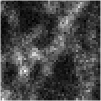
\includegraphics[width=0.18\textwidth]{blinking-1-6a.png}
		\hfill
		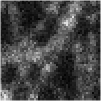
\includegraphics[width=0.18\textwidth]{blinking-1-6b.png}
		\hfill
		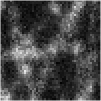
\includegraphics[width=0.18\textwidth]{blinking-1-6c.png}
		\hfill
		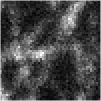
\includegraphics[width=0.18\textwidth]{blinking-1-6d.png}
		\hfill
		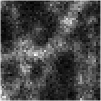
\includegraphics[width=0.18\textwidth]{blinking-1-6e.png}
		\hfill
	}
	\caption{Пример серии изображений, полученных с использованием мигающих флуорофоров}
	\label{fig:blinking-samples}
\end{figure}

В последние годы для этой области микроскопии было разработано множество алгоритмов, основанных на различных подходах, для решения задачи построения резкого изображения с высоким разрешением на основе серии снимков. В частности, алгоритмы PALM~\cite{betzig2006imaging} и STORM~\cite{rust2006sub} использует редко мигающие красители, чтобы находить центры отдельных пятен в каждом кадре и строить карту молекул флуорофора. Ограничением является требование низкой частоты мигания молекул и длинных серий снимков для визуализации всех участков изучаемого объекта.

Метод SOFI~\cite{dertinger2009fast, dertinger2010achieving} использует корреляцию и полуинварианты (см.~\cite{75086, малахов1978кумулянтный}) пикселей для уменьшения размытия и увеличения разрешения изображения. Однако он чувствителен к шуму, поэтому требует длинных последовательностей данных, а также этапа устранения размытия.

В то время как полуинварианты, используемые в SOFI, оценивают только часть ковариационной матрицы серии изображений, SPARCOM~\cite{Solomon:18} полностью использует эту матрицу и использует предположение о разреженности в пространстве корреляций сигналов флуорофоров для достижения более высокого пространственного разрешения и уменьшения требований к длине последовательности изображений.

Метод MUSICAL~\cite{agarwal2016multiple} вдохновлён алгоритмом обработки радиолокационных сигналов MUSIC~\cite{schmidt1986multiple}. Он использует собственные вектора серии изображений для построения карты флуорофоров с высоким разрешением.

Другой подход предложен авторами 3B~\cite{cox2012bayesian}. Их метод байесовского анализа мигания и выгорания моделирует изменение состояний флуорофоров и вычисляет расположение молекул. Однако его вычислительная сложность очень высока, и для практического использования этого алгоритма требуется кластерный компьютер.

Для этой задачи также разработаны методы, основанные на глубоком обучении. Например, свёрточная нейтральная сеть Deep"~STORM~\cite{Nehme:18} основана на архитектуре кодировщик"=декодировщик и напрямую создаёт изображения с высоким разрешением, тогда как метод DLBI~\cite{10.1093/bioinformatics/bty241} сочетает в себе как глубокое обучение, так и байесовский вывод, который уточняет результат нейронной сети. 

Однако проблема всё ещё остаётся открытой, и требуется более высокая производительность алгоритмов улучшения изображения. Поэтому в данной диссертационной работе разработан регуляризирующий метод реконструкции изображения повышенного разрешения и проведено сравнение его эффективности с некоторыми другими современными методами.

\section{Математическая модель искажения изображения}

Модель искажения изображения флуоресцентной микроскопии имеет вид:

\begin{equation*}
	y_{ij} = \left(Kx+n\right)_{ij},\quad K=DB,
\end{equation*}

\noindent где $x$ "--- исходное резкое изображение высокого разрешения, $y$ "--- наблюдаемое изображение, $K$ "--- оператор размытия и понижения разрешения, действие которого эквивалентно последовательному действию оператора размытия $B$ и оператора понижения разрешения $D$ (производящего, например, усреднение групп соседних пикселей или простое прореживание пиксельной сетки изображения), а $n$ "--- аддитивный шум с нормальным распределением.

\subsection{Модель размытия изображения} \label{sec:image-blur-model}

Рассматриваемая модель размытия изображения имеет вид свёртки изображения с ядром размытия:

\begin{equation*}
%	I^\prime \left( x, y \right)=\left(K\ast I+N\right)\left(x,y\right)=\int_{-\infty}^{\infty}\int_{-\infty}^{\infty}{K\left(s,t\right)\ I\left(x-s,y-t\right)\ ds\ dt}+N(x,y),
	x^\prime \left(p, q\right) = \left(B \ast x\right) \left(p, q\right) = \int_{-\infty}^{\infty}\int_{-\infty}^{\infty}{B\left(s,t\right)\ x\left(p-s,q-t\right)\ ds\ dt},
\end{equation*}

\noindent где $x$ "--- исходное резкое изображение, $x^\prime$ "--- искажённое изображение, $B$ "--- ядро размытия (англ.~point spread function, PSF), что в дискретном случае принимает вид:

\begin{equation*}
	x^\prime_{i,j} = \left(B \ast x\right)_{i,j} = \sum_{k=-\infty}^{\infty} \sum_{p=-\infty}^{\infty}{B_{k,p}\ x_{i-k,j-p}}.
\end{equation*}

\subsection{Модель ядра размытия} \label{sec:microscope-psf}

Получившее широкое распространение конфокальные лазерные микроскопы позволяют, сканируя образец лазерным лучом, возбуждать молекулы флуорофора в малых областях образца и получать в итоге более чёткое изображение, чем  при подсветке всего образца сразу. Кроме того, флуоресцентное излучение со смежных слоёв образца, находящихся не в фокусе объектива, частично отсекается точечной диафрагмой, расположенной перед приёмником света. Базовая схема такого микроскопа представлена на Рис.~\ref{fig:scanning-microscope-scheme}.

\begin{figure}[ht]
	\centerfloat{
		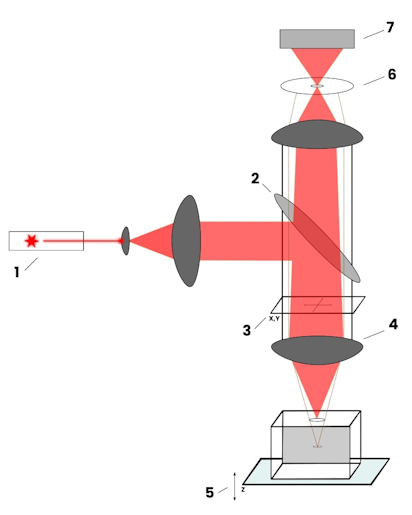
\includegraphics[height=0.4\textheight]{scanning-microscope-scheme.png}
	}
	\caption{Базовая схема конфокального лазерного сканирующего микроскопа. 1 "--- источник лазерного излучения; 2 "--- дихроичное зеркало, отражающее излучение с определённой длиной волны; 3 "--- механизм управления направлением луча лазера; 4 "--- линза объектива; 5 "--- механизм управления расстоянием от объектива до образца; 6 "--- точечная диафрагма; 7 "--- детектор флуоресцентного излучения.}
	\label{fig:scanning-microscope-scheme}
\end{figure}

%Благодаря поточечной подсветке, ядро размытия в лазерном сканирующем микроскопе $PSF_{eff}\left(r\right)$ определяется произведением ядра размытия лазерного луча подсветки образца $PSF_{exc}\left(r,r_{0,exc}\right)$ и ядра размытия объектива $PSF_{em}\left(r,r_{0,em}\right)$. Каждое из этих ядер симметрично и задаётся формулами:

Благодаря поточечной подсветке, ядро размытия в лазерном сканирующем микроскопе $PSF_{eff}$ определяется произведением ядра размытия лазерного луча подсветки образца $PSF_{exc}$ и ядра размытия объектива $PSF_{em}$. Каждое из этих ядер симметрично и задаётся формулами:

\begin{align*}
	&PSF\left(r\right) = I_0 \cdot \left(\frac{2\cdot J_1\left(v\right)}{v}\right)^2, \\
	&v=\frac{2\cdot\pi\cdot d_a\cdot\left|r-r_0\right|}{\lambda}, \\
	&J_1(v)=\sum_{n=0}^{\infty}{\left(-1\right)^n\frac{x^{2n+1}}{2^{2n+1}n!\left(n+1\right)!}},
\end{align*}

\noindent где $I_0$ "--- нормирующий множитель, $J_1$ "--- функция Бесселя первого рода первого порядка, $\lambda$ "--- длина волны лазера подсветки или флуоресцентного излучения, $r$ "--- точка в плоскости изображения, $r_0$ "--- центр ядра в плоскости изображения.

Характер отдельного ядра размытия $PSF\left(r\right)$ определён дифракцией света, а само такое ядро называется диском Эйри. Расстояние $d_a$ между ближайшими к центру этого ядра нулями называется диаметром диска Эйри (англ.~airy unit, AU) и равно $\frac{\mu\cdot \lambda}{\pi \cdot A_n}$, где $\mu$ "--- наименьший положительный нуль функции Бесселя первого рода первого порядка, а $A_n$ "--- числовая апертура фокусирующей линзы.

Итоговое ядро размытия получаемого микроскопом изображения имеет вид $PSF_{eff}\left(r\right)=PSF_{exc}\left(r,r_{0,exc}\right)\cdot PSF_{em}\left(r,r_{0,em}\right)$, где $r$ "--- точка на изображении, $r_{0,exc}$, $r_{0,em}$ "--- центры ядер размытия лазера подсветки и флуоресцентного излучения соответственно (см.~Рис.~\ref{fig:blinking-psf}).

\section{Описание данных}

\subsection{Источники данных}

Искусственные данные были подготовлены с помощью инструмента для симуляции процесса получения серий снимков мигающей флуоресцентной микроскопии SOFI Simulation Tool~\cite{10.1371/journal.pone.0161602}, модифицированном для получения структуры в виде сходящихся отрезков.

Экспериментальные данные были получены в сотрудничестве с биологами Токийского университета с помощью микроскопа Zeiss~LSM~880 с детектором Airyscan~\cite{weisshart2014basic}, состоящем из 32 сенсоров, и мигающего флуоресцентного красителя HMSiR~\cite{uno2014spontaneously}. Серия снимков представляла собой 32 синхронных серии с разных сенсоров микроскопа, которые были предварительно совмещены.

\subsection{Детектор Airyscan}

%В данной главе задача повышения качества снимков решается для лазерного сканирующего микроскопа Zeiss~LSM~880, на котором установлен объектив с шестидесятикратным увеличением и детектор Airyscan~\cite{weisshart2014basic}, состоящий из 32 сенсоров, изображения с которых совмещаются для предварительного повышения резкости итогового снимка. Для такой системы задача устранения размытия становится крайне важной.

Так как итоговое ядро размытия лазерного сканирующего микроскопа представляет собой произведение ядра размытия луча подсветки и ядра размытия излучения объекта (см.~п.~\ref{sec:microscope-psf}), то при смещении детектора излучённого света в сторону от оптической оси микроскопа результирующее ядро размытия будет меняться, становясь более узким в центральной части, но приобретая более весомый <<хвост>>, как показано на Рис.~\ref{fig:blinking-psf-displacement}. На этом принципе основана работа детектора Airyscan.

\begin{figure}[ht]
	\hfill
	\centering
	\begin{minipage}{0.45\textwidth}
		\centering
		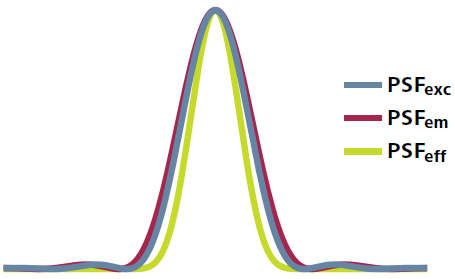
\includegraphics[width=0.9\linewidth]{blinking-1-1.png}
		\captionof{figure}{Нормированные профили ядер размытия лазера подсветки ($PSF_{exc}$), объектива ($PSF_{em}$) и микроскопа ($PSF_{eff}$)}
		\label{fig:blinking-psf}
	\end{minipage} \hfill
	\begin{minipage}{0.45\textwidth}
		\centering
		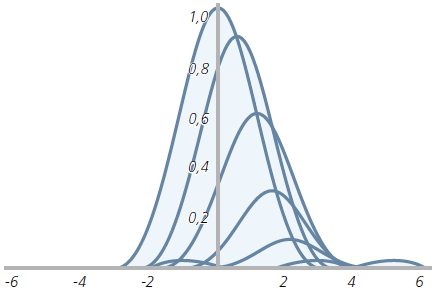
\includegraphics[width=0.9\linewidth]{blinking-1-2.png}
		\captionof{figure}{Изменение профиля ядра размытия при смещении детектора излучаемого образцов света от оптической оси}
		\label{fig:blinking-psf-displacement}
	\end{minipage}
	\hfill
\end{figure}

Изображение получается синхронно 32 детекторами: одним центральным и расположенными вокруг него тремя кольцами детекторов (Рис.~\ref{fig:blinking-airyscan}). Суммарный размер детектора Airyscan равен 1.25 диаметра диска Эйри, а размер одного элемента равен $\frac{1.25\ d_a}{6}$. Затем изображения с детекторов смещаются в сторону оптической оси с тем, чтобы положения максимумов ядер размытия детекторов совпали. Этот процесс называется переназначением пикселей (англ.~pixel reassignment)~\cite{sheppard2013superresolution}. Величина смещения $v$ изображения с одного детектора к центру определяется по формулам:

\begin{subequations}
	\begin{align}
		&v=-\frac{1}{1+\beta}\cdot\ \frac{1.25\ d_a}{6}\cdot v_d,  \nonumber \\
		&\beta=\frac{\lambda_{em}}{\lambda_{exc}},  \nonumber
	\end{align}
\end{subequations}

\noindent где $v_d$ "--- относительное смещение детектора $d$ от оптической оси в размерах детектора, $\lambda_{em}$ и $\lambda_{exc}$ "--- длины волн излучённого света и подсветки. После этого изображения суммируются, образуя изображение с более узким ядром размытия (Рис.~\ref{fig:blinking-psf-comparison}) и повышенным отношением уровня сигнала к шуму.

\begin{figure}[ht]
	\centering
	\hfill
	\begin{minipage}{0.45\textwidth}
		\centering
		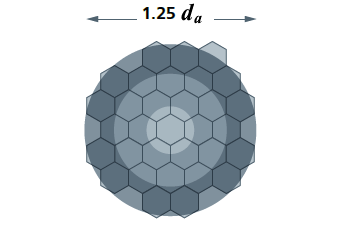
\includegraphics[width=\linewidth]{blinking-1-3-ru.png}
		\captionof{figure}{Схема детектора Airyscan. Сенсоры расположены в центрах правильных шестиугольников}
		\label{fig:blinking-airyscan}
	\end{minipage} \hfill
	\begin{minipage}{0.45\textwidth}
		\centering
		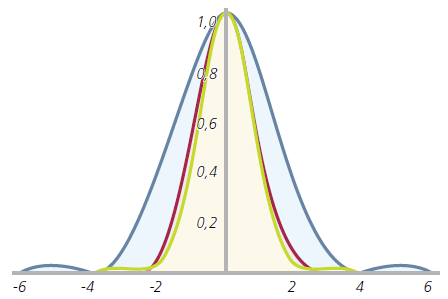
\includegraphics[width=\linewidth]{blinking-1-4.png}
		\captionof{figure}{Нормированные профили ядер размытия обычного широкопольного (синий), конфокального сканирующего (красный) микроскопов и микроскопа с детектором Airyscan (зелёный)}
		\label{fig:blinking-psf-comparison}
	\end{minipage}
	\hfill
\end{figure}

За счёт такого подхода достигается резкость конфокальных сканирующих микроскопов одновременно с высоким уровнем сигнала обычных широкопольных микроскопов, что позволяет делать длинные серии снимков с высокой частотой кадров. Примеры ядер размытия для центрального элемента и элементов каждого из колец Airyscan представлены на Рис.~\ref{fig:blinking-airyscan-psf-samples}.

\begin{figure}[ht]
	\centerfloat{
		\hfill
		\subcaptionbox[List-of-Figures entry]{Центр}{%
			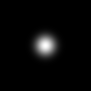
\includegraphics[width=0.2\textwidth]{blinking-1-5a.png}}
		\hfill
		\subcaptionbox{Внутреннее кольцо}{%
			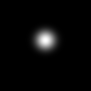
\includegraphics[width=0.2\textwidth]{blinking-1-5b.png}}
		\hfill
		\subcaptionbox{Среднее кольцо}{%
			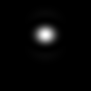
\includegraphics[width=0.2\textwidth]{blinking-1-5c.png}}
		\hfill
		\subcaptionbox{Внешнее кольцо}{%
		
\includegraphics[width=0.2\textwidth]{blinking-1-5d.png}}
		\hfill
	}
	\caption{Нормированные по яркости ядра размытия для элементов из разных слоёв детектора Airyscan}
	\label{fig:blinking-airyscan-psf-samples}
\end{figure}

\section{Рассматриваемые методы}

В данном параграфе рассматривается ряд современных методов повышения разрешения и резкости флуоресцентных изображений, полученных с использованием мигающих красителей. Далее следует описание их базовых принципов.

\subsection{Визуализация оптических флуктуаций сверхвысокого разрешения (SOFI)}

Метод SOFI (super"=resolution optical fluctuation imaging)~\cite{dertinger2009fast,dertinger2010achieving} основан на рассмотрении интенсивностей излучения молекул флуорофора как независимых случайных величин и для получения резкого изображения повышенного разрешения использует полуинварианты (англ.~cumulants) "--- коэффициенты разложения в степенной ряд логарифма характеристической функции случайной величины, которые также могут быть выражены через моменты этой случайной величины (см.~\cite{75086, малахов1978кумулянтный}).

В рамках этого подхода рассматриваются $N$ независимо мигающих флуорофоров, находящихся в позициях $\mathbf{r}_k$. Их яркости меняются со временем по закону $\varepsilon_k\cdot s_k(t)$, а итоговая интенсивность в позиции $r$ задаётся следующим образом:

\begin{equation}
	\sum_{k=1}^{N}{\delta(\mathbf{r}-\mathbf{r}_k)\cdot\varepsilon_k\cdot s_k(t)}, \quad \delta\left(\mathbf{r}-\mathbf{r}_k\right)=
	\begin{cases}
		1,\ \mathbf{r}=\mathbf{r}_k, \\
		0,\ \mathbf{r}\neq\mathbf{r}_k,
	\end{cases} \nonumber
\end{equation}	

\noindent где $\varepsilon_k$ "--- постоянная яркость молекулы красителя, а $s_k(t)$ "--- зависящая от времени функция.

Считая, что позиции молекул флуорофора не меняются со временем, а ядро размытия изображения $U(\mathbf{r})$ одинаково для всех участков изображения, интенсивность $F(\mathbf{r},t)$ в позиции $r$ в момент времени $t$ можно записать в следующем виде:

\begin{equation}
	F\left(\mathbf{r},t\right)=\sum_{k=1}^{N}{U(\mathbf{r}-\mathbf{r}_k)\cdot\varepsilon_k\cdot s_k(t)}. \nonumber
\end{equation}

Изменение интенсивности также может быть выражено как флуктуации с нулевым математическим ожиданием:

\begin{align*}
	\delta F\left(\mathbf{r},t\right) &= F\left(\mathbf{r},t\right)-\langle F\left(\mathbf{r},t\right) \rangle_t = \\
	&= \sum_{k} {U\left(\mathbf{r} - \mathbf{r}_k\right) \cdot \varepsilon_k \cdot \left[ s_k\left(t\right)- \langle s_k\left(t\right) \rangle_t \right]} = \\
	&= \sum_{k} {U\left(\mathbf{r} - \mathbf{r}_k\right) \cdot \varepsilon_k \cdot \delta s_k \left(t\right)},
\end{align*}

\noindent где $\langle \ldots \rangle_t$ означает усреднение по времени. Тогда результат работы алгоритма SOFI 2"~порядка определяется значением автокорреляционной функции изменения интенсивности $\delta F\left(\mathbf{r},t\right)$ и задаётся формулой:

\begin{align*}
	G_2\left(\mathbf{r},\tau\right) &= \langle \delta F\left(\mathbf{r},t+\tau\right)\cdot\delta F\left(\mathbf{r},t\right) \rangle_t = \\
	&= \sum_{j,k} {U\left(\mathbf{r}-\mathbf{r}_j\right)U\left(\mathbf{r}-\mathbf{r}_k\right)\cdot\varepsilon_j\cdot\varepsilon_k\cdot \langle \delta s_j\left(t+\tau\right)\delta s_k\left(t\right) \rangle_t} = \\
	&= \sum_{k} {U^2\left(\mathbf{r}-\mathbf{r}_k\right)\cdot\varepsilon_k^2\cdot \langle \delta s_k\left(t+\tau\right)\delta s_k\left(t\right) \rangle_t}.
\end{align*}

Последний переход обусловлен независимостью сигналов от молекул красителя из разных участков образца, перекрёстные члены суммы принимают нулевые значения для всех $\mathbf{r}$ и $\tau$.

Как видно из последнего уравнения, автокорреляционная функция имеет вид свёртки некоторого резкого изображения, задаваемого формулой $\sum_{k=1}^{N} {\delta(\mathbf{r}-\mathbf{r}_k)\cdot\varepsilon_k^2\cdot \langle \delta s_k\left(t+\tau\right)\delta s_k\left(t\right) \rangle_t}$, с квадратом исходного ядра размытия. Благодаря тому, что полная ширина на полувысоте (англ.~full width at half maximum, FWHM) возведённого в степень $\alpha>1$ ядра меньше, чем у исходного ядра, результат работы алгоритма SOFI обладает более высокой резкостью, чем необработанное изображение, а также позволяет достичь лучшего результата при дальнейшем восстановлении размытого изображения из-за усиленных высоких частот в спектре изображения. В частности, в случае гауссовского размытия квадрат ядра размытия в $\sqrt{2}$ раз уже самого ядра.

Можно заметить, что при $\tau=0$ значение $G_2\left(\mathbf{r},\tau\right)$ совпадает с полуинвариантом 2"~го порядка, который равен дисперсии величины $\delta F\left(\mathbf{r},t\right)$.

Для порядков SOFI выше второго используется не автокорреляционная функция, а полуинварианты соответствующих порядков, так как в противном случае перекрёстные члены в сумме остаются.

Хотя теоретического ограничения на степень повышения резкости нет, на практике используются полуинварианты порядков не выше четвёртого из-за роста влияния шума на результат с ростом порядка полуинварианта. А поскольку результат преобразования содержит не яркость молекул, а значения, зависящие от колебания яркости, которые могут быть в том числе равными нулю или меньше него, то только полуинвариант второго порядка (дисперсия яркости) даёт наиболее устойчивый результат с минимальной потерей данных и деталей изображения. Это и обусловило выбор второго порядка SOFI для проведения сравнения методов.

При замене полуинвариантов на смешанные полуинварианты (англ.~joint cumulants) "--- коэффициенты разложения в степенной ряд логарифма характеристической функции случайного вектора, составленного из нескольких случайных величин~\cite{малахов1978кумулянтный} "--- получившийся алгоритм XC"~SOFI $n$"~го порядка, помимо повышения резкости, обеспечивает и повышение разрешения в $n$ раз. В этом случае в преобразовании участвует несколько соседних пикселей изображения. В частности, для второго порядка получаем следующее выражение:

\begin{align*}
	&{XC}_2\left(\mathbf{r}_1,\mathbf{r}_2,\tau_1,\tau_2\right) = \\
	&= \sum_{i=1}^{N} {U\left(\mathbf{r}_1-\mathbf{r}_i\right)U\left(\mathbf{r}_2-\mathbf{r}_i\right)\cdot\varepsilon_k^2\cdot \langle \delta s_i\left(t+\tau_1\right)\delta s_i\left(t+\tau_2\right) \rangle_t} = \\
	&= U\left(\frac{\mathbf{r}_1-\mathbf{r}_2}{\sqrt2}\right) \sum_{i=1}^{N} {U^2\left(\frac{\mathbf{r}_1+\mathbf{r}_2}{2}-\mathbf{r}_i\right)\cdot\varepsilon_i^2\cdot \langle \delta s_i\left(t+\tau_1\right)\delta s_i\left(t+\tau_2\right) \rangle_t}.
\end{align*}

Отсюда видно, что:
\begin{enumerate}[beginpenalty=10000]
	\item Позиция результирующего пикселя лежит между двумя пикселя, участвующими в преобразовании.
	\item Результирующий пиксель имеет дополнительный множитель $U\left(\frac{\mathbf{r}_1-\mathbf{r}_2}{\sqrt2}\right)$, поэтому необходимо произвести перевзвешивание результирующего изображения для приведения уровня яркости разных групп пикселей к одному. При неизвестном ядре размытия это можно сделать, например, нормировав яркости пикселей каждой группы на среднее отклонение или математическое ожидание их яркостей.
\end{enumerate}

Для более высоких порядков формула приобретает вид:	

\begin{equation*}
	\begin{multlined}
		{XC}_n\left(\mathbf{r}_1,{\ldots,\mathbf{r}}_n,\tau_1,{\ldots,\tau}_n \right) = \\
		= \prod_{j<l}^{n}{U\left(\frac{\mathbf{r}_j-\mathbf{r}_l}{\sqrt n}\right)} \cdot \sum_{i=1}^{N}{U^n\left(\frac{\sum_{k}^{n}\mathbf{r}_k}{n}-\mathbf{r}_i \right)\cdot\varepsilon_i^n\cdot w_i(\tau_1,\ldots,\tau_n)},
	\end{multlined}
\end{equation*}

\noindent где $w_i$ "--- смешанный полуинвариант функций $s_i(t)$ порядка $n$.

\subsection{Алгоритм классификации множественных сигналов для флуоресцентной микроскопии сверхвысокого разрешения MUSICAL}

Метод повышения разрешения и резкости изображений MUSICAL (Multiple signal classification algorithm for super-resolution fluorescence microscopy)~\cite{agarwal2016multiple} основан на методе разделения нескольких сигналов MUSIC~\cite{schmidt1986multiple}.

В рамках этого метода интенсивность $n$"~го пикселя $k$"~го кадра ($1\le k\le K$, где $K$ "--- общее число изображений в обрабатываемой серии) задаётся формулой

\begin{equation}
	I_k\left({\vec{r}}_n\right)=\int_{y_n-\frac{w}{2}}^{y_n+\frac{w}{2}}\int_{x_n-\frac{w}{2}}^{x_n+\frac{w}{2}}\sum_{m=1}^{M}{G\left({\vec{r}}_n,{\vec{r}}_m^{\,\prime}\right)\ s_m\left(k\right)\ dx\ dy}\approx\sum_{m=1}^{M}{w^{2\ }G\left({\vec{r}}_n,{\vec{r}}_m^{\,\prime}\right){\ s}_m\left(k\right)}, \nonumber
\end{equation}	

\noindent где ${\vec{r}}_n=(x_n,y_n)$ "--- позиция $n$"~го пикселя в плоскости изображения, $w$ "--- длина его стороны, ${\vec{r}}_m^{\,\prime}$ "--- позиция $m$"~го флуорофора в плоскости образца, $s_m\left(k\right)\geq0$ "--- суммарное излучение от $m$"~го флуорофора за время выдержки $k$"~го кадра (при этом $\exists k: {s}_m\left(k\right)>0$), а $G\left(\vec{r},{\vec{r}}^{\,\prime}\right)\ \geq\ 0$ "--- функция, определяющая ядро размытия, отображающая интенсивность излучения из точки ${\vec{r}}^{\,\prime}$ в плоскости образца в точку $\vec{r}$ в плоскости изображения.

Таким образом, интенсивности всех пикселей $k$"~го изображения могут быть записаны в виде матричного уравнения: ${\overline{I}}_k=\mathbf{G}{\overline{s}}_k$, где

\begin{align*}
	&{\overline{I}}_k=\left[
		\begin{array}{cccc}
			I_k\left({\vec{r}}_1\right) & I_k\left({\vec{r}}_2\right) & \cdots & I_k\left({\vec{r}}_N\right)
		\end{array}
	\right]^\mathrm{T}, \\
	&\mathbf{G}=w^2 \left[
		\begin{array}{cccc}
			\overline{G}\left({\vec{r}}_1^{\,\prime}\right) & \overline{G}\left({\vec{r}}_2^{\,\prime}\right) & \cdots & \overline{G}\left({\vec{r}}_M^{\,\prime}\right)
		\end{array}
	\right], \\
	&\overline{G}\left({\vec{r}}^{\,\prime}\right)=\left[
		\begin{array}{cccc}
			G\left({\vec{r}}_1,{\vec{r}}^{\,\prime}\right) & G\left({\vec{r}}_2,{\vec{r}}^{\,\prime}\right) & \cdots & G\left({\vec{r}}_N,{\vec{r}}^{\,\prime}\right)
		\end{array}
	\right]^\mathrm{T}, \\
	&{\overline{s}}_k=\left[
		\begin{array}{cccc}
			s_1\left(k\right) & s_2\left(k\right) & \cdots & s_M\left(k\right)
		\end{array}
	\right]^\mathrm{T}.
\end{align*}

Полный набор изображений может быть записан матрицей

\begin{equation*}
	\mathbf{I} = \left[
		\begin{array}{cccc}
			{\overline{I}}_1 & {\overline{I}}_2 & \cdots & {\overline{I}}_K
		\end{array}
	\right] = \mathbf{G} \cdot \left[
		\begin{array}{cccc}
			{\overline{s}}_1 & {\overline{s}}_2 & \cdots & {\overline{s}}_K
		\end{array}
	\right].
\end{equation*}

Отсюда видно, что каждый столбец матрицы $\mathbf{I}$ "--- это линейная комбинация столбцов матрицы $\mathbf{G}$, а пространство столбцов матрицы $\mathbf{I}$, являющееся линейной оболочкой полученных изображений, определяется пространством столбцов матрицы $\mathbf{I}$. Одновременно с этим пространство столбцов матрицы $\mathbf{I}$ задаётся левыми сингулярными векторами из сингулярного разложения этой матрицы, у которых соответствующие им сингулярные числа не равны нулю: $\left\{{\overline{u}}_{\sigma_i\neq0}\right\}$.

Если $\mathbf{I}$ "--- матрица неполного ранга, то существует линейное пространство векторов $\left\{{\overline{u}}_{\sigma_i=0}\right\}$, ортогональное пространству столбцов матрицы $\mathbf{I}$, и выполняется $\overline{G}\left({\vec{r}}_m^{\,\prime}\right) \cdot {\overline{u}}_{\sigma_i=0}=0$ для всех $m$. При условии, что флуорофоры мигают независимо, одному элементу из $\left\{\overline{G}\left({\vec{r}}_m^{\,\prime}\right); m=\overline{1;M}\right\}$ соответствует один и только один элемент из $\left\{{\overline{u}}_{\sigma_i\neq0}\right\}$. Поэтому вектора $\overline{G}\left({\vec{r}}^{\,\prime}\right)$ для позиций ${\vec{r}}^{\,\prime} \notin \left\{{\vec{r}}_m^{\,\prime},\ m=\overline{1;M}\right\}$ имеют ненулевую проекцию на линейное пространство векторов $\left\{{\overline{u}}_{\sigma_i=0}\right\}$.

В случае полного ранга выбирается некоторый порог $\sigma_0$ и за базис пространства столбцов матрицы берётся множество $\left\{{\overline{u}}_{\sigma_i\geq\sigma_0}\right\}$, а за базис ортогонального сигналу пространства "--- $\left\{{\overline{u}}_{\sigma_i<\sigma_0}\right\}$. Обусловлен такой подход тем, что разные вектора ${\overline{u}}_{\sigma_i}$ соответствуют разным структурным деталям изображений, соответствующие им $\sigma_i^2$ определяют энергию (силу) этих векторов, а вектора с низкой энергией могут быть сильно искажены шумом и не могут считаться надёжными при восстановлении изображения высокого разрешения.

Для проверки условий принадлежности вектора $\overline{G}\left({\vec{r}}^{\,\prime}\right)$ к $\left\{\overline{G}\left({\vec{r}}_m^{\,\prime}\right); m=\overline{1;M}\right\}$ в MUSICAL используется индикаторная функция с параметром $\alpha$, отвечающим за контраст:

\begin{align*}
	&f\left({\vec{r}}_{test}^{\,\prime}\right) = \left(\frac{d_{PR}\left({\vec{r}}_{test}^{\,\prime}\right)} {d_{PN}\left({\vec{r}}_{test}^{\,\prime}\right)}\right)^\alpha, \\
	&d_{PR}\left({\vec{r}}_{test}^{\,\prime}\right) = \sqrt{\sum_{\sigma_i\geq\sigma_0}{\lVert \overline{G}\left({\vec{r}}_{test}^{\,\prime}\right)\cdot{\overline{u}}_i \rVert}^2}, \\
	&d_{PN}\left({\vec{r}}_{test}^{\,\prime}\right) = \sqrt{\sum_{\sigma_i<\sigma_0}{\lVert \overline{G}\left({\vec{r}}_{test}^{\,\prime}\right)\cdot{\overline{u}}_i \rVert}^2}.
\end{align*}

Значения такой индикаторной функции будут тем больше, чем ближе точка ${\vec{r}}^{\,\prime}$ к позиции одного из $m$ флуорофоров. Посчитав значения этой функции для всех пикселей изображения высокого разрешения, можно построить своего рода карту расположения молекул флуорофоров.

Для ускорения работы алгоритма и устойчивости определения базиса пространства сигнала алгоритм MUSICAL обрабатывает изображение не целиком, а с использованием скользящего окна, сопоставимого по размеру с диаметром ядра размытия, с дальнейшим усреднением значений индикаторной функции в областях перекрытия окон.

\subsection{Байесовский анализ мигания и выгорания 3B}

Ещё одним рассмотренным методом является метод локализации молекул флуорофора с помощью байесовского алгоритма локализационной микроскопии~\cite{cox2012bayesian}. Метод использует скрытую марковскую модель для представления переходов флуорофора между тремя состояниями (излучает, не излучает, разрушен) и делает вывод о присутствии флуорофора в точке на основе отношения вероятности его присутствия (событие $\mathcal{F}$) в этой точке при учёте наблюдаемых данных $D$ к вероятности его отсутствия (событие $\mathcal{N}$) при тех же данных: $\frac{p\left(\mathcal{F}\middle| D\right)}{p\left(\mathcal{N}\right|D)} = \frac{p\left(D\middle|\mathcal{F}\right)p\left(\mathcal{F}\right)} {p\left(D\middle|\mathcal{N}\right)p\left(\mathcal{N}\right)}$. Так как $p\left(\mathcal{F}\right)$ и $p\left(\mathcal{N}\right)$ постоянные, то оценить нужно только вероятности $p\left(D\middle|\mathcal{F}\right)$ и $p\left(D\middle|\mathcal{N}\right)$. Последнее "--- это вероятность наблюдения данных при учёте наличия в них только шума известной модели (например, шума с нормальным распределением). Первая величина вычисляется следующим образом:

\begin{equation*}
	p\left(D\middle|\mathcal{F}\right)=\int_{a\in\mathbb{R}^4}\int_{b\in\mathbb{Z}_3^N}{p\left(D,a,b\middle|\mathcal{F}\right)\ db\ da},
\end{equation*}

\noindent где $a$ "--- 4 параметра каждого флуорофора (координаты в плоскости изображения, яркость и размер), а $b$ "--- набор состояний флуорофора в каждом кадре. Вероятность $p\left(D,a,b\middle|\mathcal{F}\right)$ равна произведению вероятности получения наблюдаемых данных при условии наличия флуорофора в рассматриваемой точке на априорные вероятности параметров $a$ и $b$. Априорные вероятности координат флуорофоров заданы равномерным распределением на рассматриваемой области изображения и нулём вне этой области. Размер изображения флуорофора имеет логнормальное априорное распределение с параметрами $\sigma=0.1$ и $\mu$ таким, чтобы мода распределения имела значение полной ширины на полувысоте заданного ядра размытия. Априорное распределение яркости флуорофора тоже логнормальное, с параметрами $\sigma=3$ и $\mu=1$. Априорное распределение состояния флуорофора в первом кадре задано так, чтобы вероятности состояний <<излучает>> и <<не излучает>> были равновероятными, а событие <<флуорофор разрушен>> "--- невозможным. Дальнейшие априорные вероятности вычисляются с использованием скрытой марковской модели в зависимости от предыдущих состояний.

С учётом всех $M$ молекул флуорофора уравнение приобретает вид:

\begin{equation*}
	p\left(D\middle|\mathcal{F}_M\right)=\int_{a\in\mathbb{R}^{4 \cdot M}}\int_{b\in\mathbb{Z}_3^{N \cdot M}}{p\left(D,a,b\middle|\mathcal{F}_M\right)\ db\ da}.
\end{equation*}	

Из-за большого объёма вычислений в случае многих молекул интегрирование по $a$ проводится приближённо методом Лапласа, а интеграл по $b$ оценивается с помощью генерации выборки $\left\{b_i\right\}_{i=1\ }^n$ методом Монте"=Карло по схеме марковской цепи и вычисления суммы

\begin{equation*}
	p\left(D\middle|\mathcal{F}_M\right)=\int_{a\in\mathbb{R}^{4 \cdot M}}\int_{b\in\mathbb{Z}_3^{N \cdot M}}{p\left(D,a,b\middle|\mathcal{F}_M\right)\ db\ da} \approx \frac{1}{n}\int_{a\in\mathbb{R}^{4 \cdot M}}{\sum_{i=1}^{n}{p\left(D,a,b_i\middle|\mathcal{F}_M\right)}}.
\end{equation*}

\section{Итерационный регуляризирующий алгоритм}

В ходе выполнения исследования нами был разработан и реализован алгоритм повышения резкости и разрешения изображений на основе байесовского подхода с использованием регуляризации.

В основе метода лежит предположение о том, что интенсивности пикселей резкого изображения можно рассмотреть как независимые случайные величины, а серию резких изображений "--- как результат серии наблюдений этих случайных величин. Влияние дифракции представлено свёрткой резкого изображения с одним и тем же ядром для всех пикселей и всех кадров, а полученные размытые снимки содержат высокочастотный шум.

В рамках предлагаемого подхода размытые зашумлённые изображения серии рассматриваются как наблюдаемые переменные, соответствующие им исходные резкие изображения "--- как скрытые, а среднее значение и дисперсия интенсивности каждого пикселя исходной серии изображений "--- как неизвестные параметры распределения интенсивности этого пикселя. Затем эти параметры распределений интенсивностей пикселей вычисляются с помощью байесовского алгоритма. При этом полученные дисперсии интенсивностей можно трактовать как высококонтрастную карту объектов с изменяющейся яркостью, на которой подсвеченный мигающим флуорофором образец будет присутствовать, а постоянный фон "--- нет.

На вход алгоритма поступает набор размытых и зашумлённых изображений $Y=\left\{y^t\right\}_{t=1}^T$, $y^t\in\mathbb{R}^l$, ему соответствует неизвестный набор резких изображений высокого разрешения $X=\left\{x^t\right\}_{t=1}^T$, $x^t\in\mathbb{R}^n$. Благодаря природе шума, его можно моделировать случайным процессом с нормальным распределением~\cite{gadsden1965some}. Поэтому в данном пункте считается, что $y^t \sim N({Kx}^t,\Theta^{-1})$, где $K\in\mathbb{R}^{n \times n}$ "--- оператор свёртки и понижения разрешения (имеет вид матрицы Тёплица с элементами ядра размытия на диагоналях, умноженной на матрицу понижения разрешения слева), а $\Theta\in\mathbb{R}^{n \times n}$ "--- обратная ковариационная матрица шума, диагональная из-за попиксельной независимости шума. Предполагается, что вследствие малого размера молекул флуорофора в каждом пикселе изображения может находиться достаточно много независимо мигающих молекул, чтобы можно было приблизить распределение суммарной яркости точки нормальным распределением: $x^t \sim N(\mu,\Lambda^{-1})$, где $\mu\in\mathbb{R}^n$ "--- средняя по всем кадрам яркость объекта, а $\Lambda\in\mathbb{R}^{n \times n}$ "--- обратная ковариационная матрица мерцания объекта.

Финальным результатом работы алгоритма являются математическое ожидание $\mu$ и диагональ ковариационной матрицы $\Lambda^{-1}$, поэлементный квадратный корень которой является стандартными отклонениями яркостей точек резких изображений. 

Рассматривая $X$, $\mu$ и $\Lambda$ как скрытые переменные, можно записать их совместное апостериорное распределение:

\begin{equation*}
	p\left(X,\mu,\Lambda\middle|Y,\Theta\right)=\frac{p\left(Y\middle|X,\Theta\right)p\left(X\middle|\mu,\Lambda\right)p\left(\mu\right)p\left(\Lambda\right)}{p\left(Y\middle|\Theta\right)}.
\end{equation*}

Для нахождения распределений $\mu$ и $\Lambda$ и матрицы $\Theta$ максимизируется правдоподобие набора кадров:

\begin{equation*}
	p\left(Y\middle|\Theta\right) \rightarrow \max_{p \left( X, \mu, \Lambda \middle| Y,\Theta \right),\Theta}
\end{equation*}
с помощью EM"~алгоритма~\cite{477e7e2b-4ded-3369-981e-9b40850a2701} с использованием аппроксимации среднего поля (англ.~mean field approximation)~\cite{bishop2006pattern}.

Апостериорное совместное распределение аппроксимируется факторизуемой плотностью вероятности:

\begin{equation*}
	p\left(X,\mu,\Lambda\middle|Y,\Theta\right)\approx q\left(X,\mu,\Lambda\right)=\prod_{t=1}^{T}{q_{1,t}\left(x^t\right)\cdot\ q_2\left(\mu\right)\cdot q_3\left(\Lambda\right)},
\end{equation*}

\noindent где в качестве множителей $q_{1,t}\left(x^t\right)$ и $q_2\left(\mu\right)$ используются нормальные распределения, а для $q_3\left(\Lambda\right)$ "--- распределение Уишарта.

Априорные распределения $p\left(\mu\right)$ и $p\left(\Lambda\right)$ в рамках исследования задаются следующим образом:

\begin{align*}
	&\mu \sim N\left(m_0,\ \eta_0^{-1}I_n\right), \\
	&\Lambda \sim W\left(W_0,\nu_0\right)=\frac{1}{C}\left|\Lambda\right|^\frac{\nu_0-n-1}{2}\exp{\left(-\frac{1}{2}tr\left[W_0^{-1}\Lambda\right]\right)},
\end{align*}

\noindent где $W(\cdots)$ "--- распределение Уишарта, $I_n$ "--- единичная матрица, $m_0\in\mathbb{R}^n$, $\eta_0,\ \nu_0\in\mathbb{R}$ и $W_0\in\mathbb{R}^{n \times n}$ "--- параметры регуляризации, а $C$ "--- нормировочная константа. Вид распределений выбран в том числе с тем, чтобы получить аналитическое решение одного из шагов алгоритма оптимизации, однако в то же время для $\mu$ после преобразований это эквивалентно добавлению стабилизатора вида $\frac{\eta_0}{2} \lVert x - m_0 \rVert^2$ на E"~шаге EM"~алгоритма.

При таких условиях совместная плотность вероятности наблюдаемых размытых зашумлённых изображений и соответствующих им <<скрытых>> резких изображений с учётом регуляризации имеет следующий вид:

\begin{align*}
	p\left(Y,X,\mu,\Lambda \middle| \Theta\right) &= \prod_{t=1}^{T} \left( \frac{\lvert\Theta\rvert \cdot \lvert\Lambda\rvert}{{2\pi}^{n}} \right)^\frac{1}{2} \exp\left(
	\begin{aligned}
		&-\frac{1}{2}\left(y^t-Kx^t\right)^T\Theta\left(y^t-Kx^t\right) - \\
		&-\frac{1}{2}\left(x^t-\mu\right)^T\Lambda\left(x^t-\mu\right)
	\end{aligned}
	\right) \cdot \\
	&\cdot \left(\frac{\eta_0}{2\pi}\right)^\frac{n}{2} \exp \left(-\frac{1}{2}\left(\mu-m_0\right)^T\eta_0I_n\left(\mu-m_0\right)\right) \cdot \\
	&\cdot \frac{1}{C}\lvert\Lambda\rvert^\frac{\nu_0-n-1}{2}\exp{\left(-\frac{1}{2}tr\left[W_0^{-1}\Lambda\right]\right)}.
\end{align*}

Тогда параметры распределений $X$, $\mu$ и $\Lambda$ и матрица $\Theta$ находятся итерационным алгоритмом, который на каждом шаге пересчитывает их по очереди в соответствии с уравнениями:

\begin{align*}
	&\log{q_{1,k}\left(x^k\right)}=\mathbb{E}_{\left\{x^{t \backslash k}\right\},\mu,\Lambda}\log{p\left(Y,X,\mu,\Lambda\mid\Theta\right)}+C_{1,k}, \\
	&\log{q_2\left(\mu\right)}=\mathbb{E}_{\left\{x^t\right\},\Lambda}\log{p\left(Y,X,\mu,\Lambda\mid\Theta\right)}+C_2, \\
	&\log{q_3\left(\Lambda\right)}=\mathbb{E}_{\left\{x^t\right\},\mu}\log{p\left(Y,X,\mu,\Lambda\mid\Theta\right)}+C_3, \\
	&\Theta=\arg{\max_\Theta{\mathbb{E}_{\left\{x^t\right\},\mu,\Lambda}\log{p\left(Y,X,\mu,\Lambda\mid\Theta\right)}}},
\end{align*}

\noindent где $\left\{C_{1,k}\right\}_{k=1}^T$, $C_2$ и $C_3$ "--- нормировочные константы.

В итоге обновление параметров происходит следующим образом:

\begin{align*}
	&q_{1,t}\left(x^t\right):\ \Sigma_{x^t}=\left(K^T\Theta K+\mathbb{E}\Lambda\right)^{-1},\ \mathbb{E}x^t=\Sigma_{x^t}\left(K^T\Theta y^t+\mathbb{E}\Lambda\cdot\mathbb{E}\mu\right); \\
	&q_2\left(\mu\right):\ \Sigma_\mu=\left(T\cdot\mathbb{E}\Lambda+\eta_0I_n\right)^{-1},\ \mathbb{E}\mu=\Sigma_\mu\left(\mathbb{E}\Lambda\cdot\sum_{t=1}^{T}{\mathbb{E}x^t}+\eta_0I_nm_0\right); \\
	&q_3\left(\Lambda\right):\ W\left(W^\prime,v^\prime\right),\ v^\prime=v_0+T \\
	&W^\prime=\left(W_0^{-1}+\sum_{t=1}^{T}\left[
	\begin{aligned}
		&\Sigma_{x^t} + \mathbb{E}x^t\left(\mathbb{E}x^t\right)^T - \mathbb{E}x^t\left(\mathbb{E}\mu\right)^T - \\
		&- \mathbb{E}\mu\left(\mathbb{E}x^t\right)^T + \Sigma_\mu + \mathbb{E}\mu\left(\mathbb{E}\mu\right)^T
	\end{aligned}
	\right]\right)^{-1}, \\
	&\mathbb{E}\Lambda=v^\prime W^\prime; \\
%	&\Theta=\left(\frac{1}{T}\sum_{t=1}^{T}\left[\left(K\mathbb{E}x^t-y^t\right)\left(K\mathbb{E}x^t-y^t\right)^T+K\Sigma_{x^t}K^T\right]\right)^{-1}. \\
	&\Theta_{ii}=\left(\frac{1}{T}\sum_{t=1}^{T}\left[\left(\left(K\mathbb{E}x^t - y^t\right)_i\right)^2 + \left(K\Sigma_{x^t}K^T\right)_{ii}\right]\right)^{-1}.
\end{align*}

Для ускорения работы алгоритма он может быть запущен без учёта повышения разрешения, а затем полученный результат после простой интерполяции может быть использован в качестве начального приближения при нахождении изображения повышенного разрешения.

\section{Эксперименты и результаты}

В ходе исследования методы SOFI, MUSICAL и разработанный итерационный алгоритм были реализованы на языке программирования Python. Для получения результатов обработки изображений алгоритмом 3B было использовано программное обеспечение от авторов этого метода (доступно по ссылке \url{http://www.coxphysics.com/3b}).

Была проведена оптимизация алгоритма SOFI для уменьшения влияния пространственно некоррелированного шума на интенсивность пикселей изображения высокого разрешения в позициях исходных пикселей путём замены вычисления автокорреляции исходных пикселей на вычисление усреднённых смешанных полуинвариантов сигналов с пикселей вокруг исходных.

Было проведено тестирования рассматриваемых алгоритмов на искусственных и реальных данных, примеры результатов обработки представлены на Рис.~\ref{fig:blinking-results-simulation}"~и"~\ref{fig:blinking-results-real}. Разработанный итерационный метод был ускорен с использованием технологии Nvidia~CUDA, тестирование остальных методов проводилось на ЭВМ с четырёхядерным процессором Intel~Core~i5~6500. Среднее время работы на представленных данных составило для XC"~SOFI порядка 2 вместе с дальнейшим устранением размытия "--- 2 секунды, для 3B "--- 45 минут, для разработанного итерационного метода "--- 2 минуты, для MUSICAL "--- 1 минута. %Использовались значения параметров $m_0 = \left(0, \ldots,  0\right)^T$, $\eta_0 = 10^{-6}$, $\v_0 = 10^{-5}$, $W_0 = 10^8 I_n$.

\begin{figure}[ht]
	\centerfloat{
		\hfill
		\subcaptionbox[List-of-Figures entry]{Карта молекул флуорофора}{%
			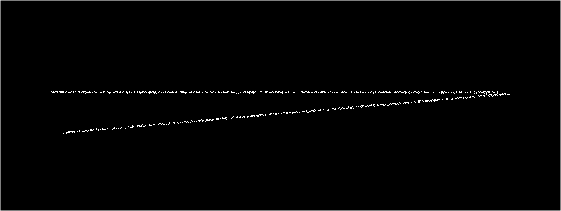
\includegraphics[width=0.3\textwidth]{blinking-1-7a.png}}
		\hfill
		\subcaptionbox{Пример одного изображения серии}{%
			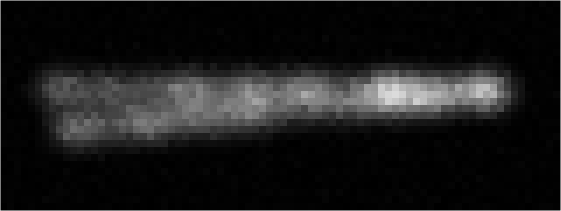
\includegraphics[width=0.3\textwidth]{blinking-1-7b.png}}
		\hfill
		\subcaptionbox{Усреднённое по времени изображение\label{fig:blinking-results-avg-sim}}{%
			
\includegraphics[width=0.3\textwidth]{blinking-1-7c.png}}
		\hfill
		\vfill
		\hfill
		\subcaptionbox{Устранение размытия на Рис.~\ref{fig:blinking-results-avg-sim} методом Люси"=Ричардсона~\cite{richardson1972bayesian}}{%
			
\includegraphics[width=0.3\textwidth]{blinking-1-7d.png}}
		\hfill
		\subcaptionbox{XC"~SOFI порядка~2\label{fig:blinking-results-sofi-2-sim}}{%
			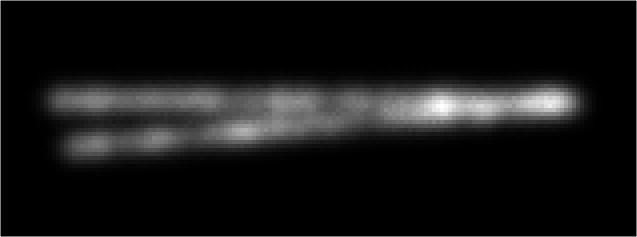
\includegraphics[width=0.3\textwidth]{blinking-1-7e.png}}
		\hfill
		\subcaptionbox{Устранение размытия на Рис.~\ref{fig:blinking-results-sofi-2-sim} методом Люси"=Ричардсона}{%
			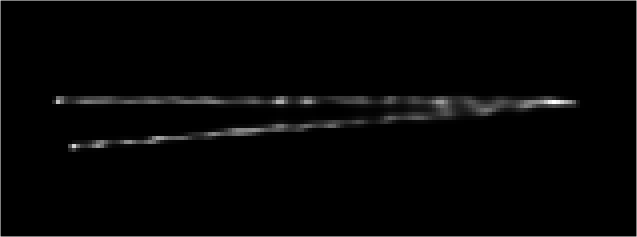
\includegraphics[width=0.3\textwidth]{blinking-1-7f.png}}
		\hfill
		\vfill
		\hfill
		\subcaptionbox{XC"~SOFI порядка~3\label{fig:blinking-results-sofi-3}}{%
			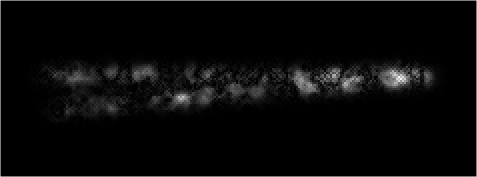
\includegraphics[width=0.3\textwidth]{blinking-1-7g.png}}
		\hfill
		\subcaptionbox{Устранение размытия на Рис.~\ref{fig:blinking-results-sofi-3} методом Люси"=Ричардсона}{%
			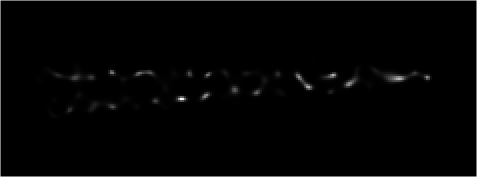
\includegraphics[width=0.3\textwidth]{blinking-1-7h.png}}
		\hfill
		\subcaptionbox{3B}{%
			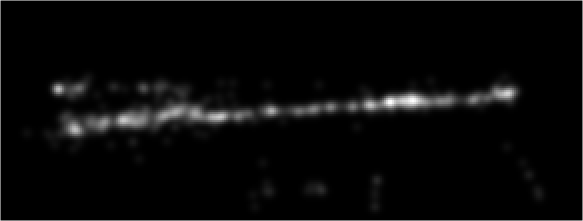
\includegraphics[width=0.3\textwidth]{blinking-1-7i.png}}
		\hfill
		\vfill
		\hfill
		\subcaptionbox{Разработанный метод, средняя яркость}{%
			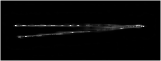
\includegraphics[width=0.3\textwidth]{blinking-1-7j.png}}
		\hfill
		\subcaptionbox{Разработанный метод, стандартные отклонения яркости}{%
			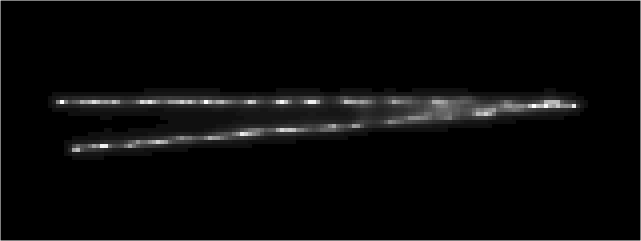
\includegraphics[width=0.3\textwidth]{blinking-1-7k.png}}
		\hfill
		\subcaptionbox{MUSICAL}{%
			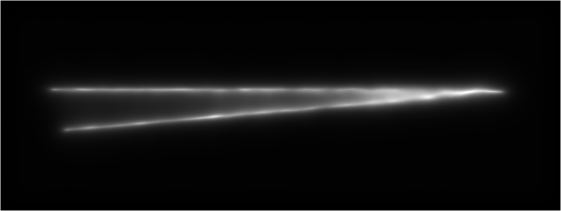
\includegraphics[width=0.3\textwidth]{blinking-1-7l.png}}
		\hfill
		\vfill
	}
	\caption{Примеры изображений из искусственного набора данных и результаты работы рассмотренных алгоритмов}
	\label{fig:blinking-results-simulation}
\end{figure}

\begin{figure}[ht]
	\centerfloat{
		\hfill
		\subcaptionbox[List-of-Figures entry]{Один кадр серии}[0.3\textwidth]{%
			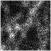
\includegraphics[width=0.2\textwidth]{blinking-1-8a.png}}
		\hfill
		\subcaptionbox{Усреднённое по времени изображение\label{fig:blinking-results-avg-real}}[0.3\textwidth]{%
			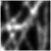
\includegraphics[width=0.2\textwidth]{blinking-1-8b.png}}
		\hfill
		\subcaptionbox{Устранение размытия на Рис.~\ref{fig:blinking-results-avg-real} методом Люси"=Ричардсона}[0.3\textwidth]{%
			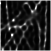
\includegraphics[width=0.2\textwidth]{blinking-1-8c.png}}
		\hfill
		\vfill
		\hfill
		\subcaptionbox{XC"~SOFI порядка~2\label{fig:blinking-results-sofi-2-real}}[0.3\textwidth]{%
			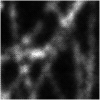
\includegraphics[width=0.2\textwidth]{blinking-1-8d.png}}
		\hfill
		\subcaptionbox{Устранение размытия на Рис.~\ref{fig:blinking-results-sofi-2-real} методом Люси-Ричардсона}[0.3\textwidth]{%
			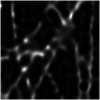
\includegraphics[width=0.2\textwidth]{blinking-1-8e.png}}
		\hfill
		\subcaptionbox{XC"~SOFI порядка~3}[0.3\textwidth]{%
			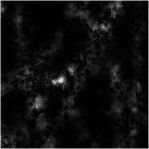
\includegraphics[width=0.2\textwidth]{blinking-1-8f.png}}
		\hfill
		\vfill
		\hfill
		\subcaptionbox{3B}[0.3\textwidth]{%
			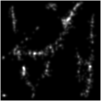
\includegraphics[width=0.2\textwidth]{blinking-1-8g.png}}
		\hfill
		\subcaptionbox{Разработанный метод, стандартные отклонения яркости}[0.3\textwidth]{%
			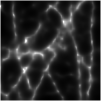
\includegraphics[width=0.2\textwidth]{blinking-1-8h.png}}
		\hfill
		\subcaptionbox{MUSICAL}[0.3\textwidth]{%
			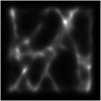
\includegraphics[width=0.2\textwidth]{blinking-1-8i.png}}
		\hfill
		\vfill
	}
	\caption{Примеры изображений из реального набора данных и результаты работы рассмотренных алгоритмов}
	\label{fig:blinking-results-real}
\end{figure}

Сравнение показало следующее:
\begin{enumerate}[beginpenalty=10000]
	\item результаты работы алгоритма 3B страдают от потери данных, получаемый результат не окупает долгое время работы алгоритма;
	\item XC"~SOFI является самым быстрым из рассмотренных, однако варианты метода порядков выше второго страдают от потери информации, а также сильно зависят от используемого алгоритма устранения размытия;
	\item разработанный метод повышения качества изображений хорошо восстанавливает детали, однако с ростом степени повышения разрешения объём вычислений растёт крайне быстро, что ограничивает возможности по повышению разрешения;
	\item алгоритм MUSICAL, несмотря на меньшую резкость результатов (наличие остаточного размытия), хорошо восстанавливает детали и может быть использован при жёстких ограничениях по времени.
\end{enumerate}

\section{Выводы}

Разработанный в рамках исследования алгоритм показал качество работы, сопоставимое с результатами алгоритма MUSICAL. Его преимуществом является большая резкость полученных клеточных структур, а также имеющие физический смысл восстановленные яркость и дисперсия яркости точек. Недостатком является высокая вычислительная сложность, не позволяющая использовать алгоритм в текущем виде для увеличения разрешения в 4 и более раз за приемлемое время.

Алгоритм MUSICAL предоставляет лучшие возможности по увеличению разрешения, однако результат содержит лишь некий показатель наличия молекул флуорофора, поэтому он может использоваться только для локализации объектов, но не определения их физических свойств.

SOFI имеет наивысшую скорость работы, однако недостаточное повышение разрешения и резкости делают нецелесообразным его использование при низком увеличении микроскопа.

%На основании вышесказанного можно сделать вывод, что в случае достаточно высокого увеличения объектива и жёстких требований по времени оптимальным алгоритмом из рассмотренных для микроскопа Zeiss~LSM~880 является SOFI. Потенциал MUSICAL должен раскрыться в случае получения снимком низкого разрешения, что позволит производить съёмку образцов быстрее при небольшой потере качества изображений. Разработанный же метод может предоставить более резкое изображение в случае изначально среднего или высокого увеличения объектива, что тоже может представлять интерес для исследователей.



\FloatBarrier           % Глава 1
\chapter{Повышение резкости медицинских изображений методом деформации пиксельной сетки}\label{ch:ch2}

На практике часто возникает необходимость повышения резкости изображений по разным причинам: из-за физических ограничений оптических систем и сенсоров камер или из-за сложных условий получения изображений. В то же время в медицине при обработке изображений важно не терять присутствующие на них детали или добавлять не существовавшие элементы или артефакты.

В отличие от наиболее распространённых методов повышения резкости (обращение свёртки, нерезкое маскирование), деформационный метод, представленный в~\cite{krylov2014gridwarping} и затем доработанный в~\cite{nasonova2014deblurred, gusev2016parallel}, не меняет значения интенсивности пикселей, а сдвигает сами пиксели в окрестности контуров изображений~(см.~Рис~\ref{fig:warping-warping-idea}). Этот подход изменяет изображение в окрестности контуров и не имеет таких недостатков, свойственных некоторым другим методам, как усиление шума и возникновение эффекта ложного оконтуривания.

\begin{figure}[ht]
	\centerfloat{
		\hfill
		\subcaptionbox[List-of-Figures entry]{Профиль контура}{%
			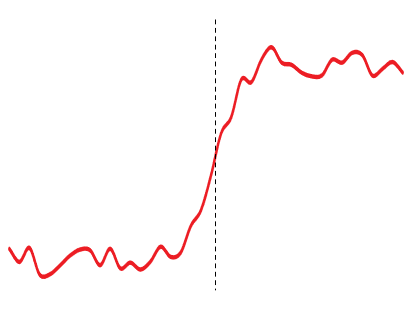
\includegraphics[width=0.3\textwidth]{warping-1-4b.png}}
		\hfill
		\subcaptionbox{Классический метод}{%
			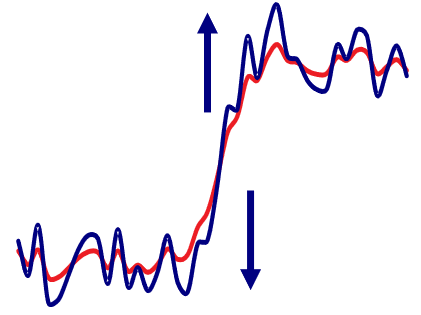
\includegraphics[width=0.3\textwidth]{warping-1-4a.png}}
		\hfill
		\subcaptionbox{Деформационный метод}{%
			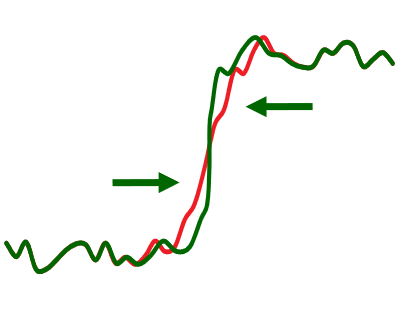
\includegraphics[width=0.3\textwidth]{warping-1-4c.png}}
		\hfill
	}
	\caption{Принцип работы классических методов и деформационного метода повышения резкости изображений}
	\label{fig:warping-warping-idea}
\end{figure}

В данной главе рассматривается деформационный алгоритм повышения резкости изображения~\cite{nasonova2014deblurred, gusev2016parallel} и набор из 24 тестовых изображений из базы TID2013~\cite{ponomarenko2015image}, размытых с разной интенсивностью с использованием трёх типов реалистичных ядер размытия. Целью является нахождение оптимальной функции смещения для каждого типа ядра размытия отдельно и для всех типов сразу.

\section{Реалистичные ядра размытия изображений}

Модель размытия изображения, рассматриваемая в этой главе, совпадает с моделью, описанной в п.~\ref{sec:image-blur-model}.

В процессе исследования рассматривались три типа ядер размытия, возникающих на практике: ядро, определяемое функцией Гаусса; и два ядра, которые часто возникают в реальных изображения, полученных с помощью фотокамер.

Ядро Гаусса выбрано по той причине, что оно соответствует одной из наиболее распространённых моделей размытия изображения, а также потому, что такое ядро (или очень близкое к нему) можно встретить в изображениях, полученных с помощью некоторых оптических систем, где дифракция света играет заметную роль (например, с помощью микроскопов).

Также, согласно модели Зейделя, существует пять видов оптических аберраций~\cite{simpkins2014parameterized}:
\begin{enumerate}[beginpenalty=10000]
	\item сферическая аберрация;
	\item кома;
	\item астигматизм;
	\item кривизна поля изображения;
	\item дисторсия.
\end{enumerate}

Ядра, отвечающие сферическим аберрациям и астигматизму, также схожи с ядром Гаусса~\cite{simpkins2014parameterized, simpkins2011modeling}, что послужило дополнительным аргументом в пользу рассмотрения этого ядра. Примеры этих искажений представлены на Рис.~\ref{fig:warping-aberrations}.

\begin{figure}[ht]
	\centerfloat{
		\hfill
		\subcaptionbox[List-of-Figures entry]{Сферическая аберрация}{%
			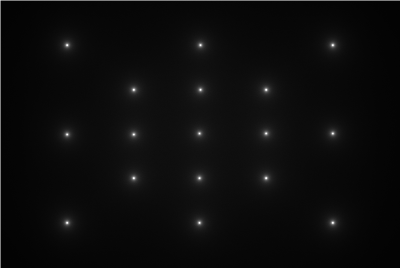
\includegraphics[width=0.45\textwidth]{warping-1-1a.png}}
		\hfill
		\subcaptionbox{Кома}{%
			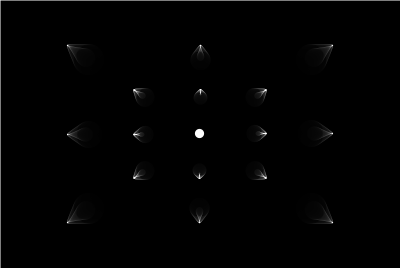
\includegraphics[width=0.45\textwidth]{warping-1-1b.png}}
		\hfill
		\vfill
		\hfill
		\subcaptionbox{Астигматизм}{%
			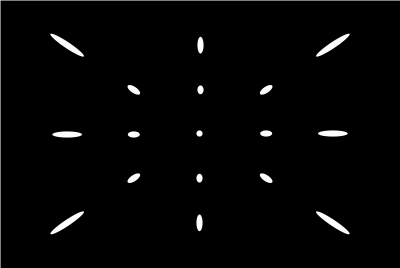
\includegraphics[width=0.45\textwidth]{warping-1-1c.png}}
		\hfill
		\subcaptionbox{Разные виды астигматизма}{%
			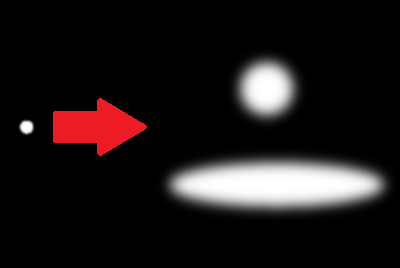
\includegraphics[width=0.45\textwidth]{warping-1-1d.png}}
		\hfill
		\vfill
		\hfill
		\subcaptionbox{Кривизна поля изображения}{%
			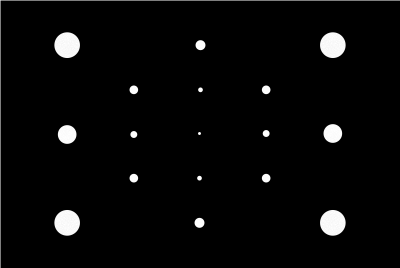
\includegraphics[width=0.45\textwidth]{warping-1-1e.png}}
		\hfill
		\subcaptionbox{Дисторсия}{%
			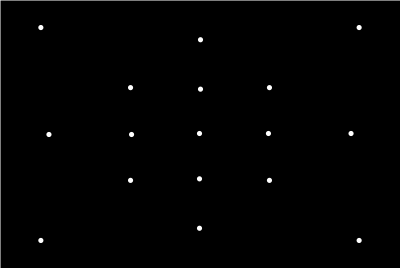
\includegraphics[width=0.45\textwidth]{warping-1-1f.png}}
		\hfill
		\vfill
	}
	\caption{Виды оптический аберраций~\cite{simpkins2011modeling}}
	\label{fig:warping-aberrations}
\end{figure}

Помимо этих пяти аберраций также встречаются просто расфокусированные изображения, либо же расфокусированные участки изображений, полученных с использованием камер с малой глубиной резкости изображаемого пространства. В таком случае полученное изображение точки имеет вид круга с приблизительно равномерной яркостью, однако также может иметь увеличение яркости в центре или на краях (что выглядит как круг с кольцом). Таким образом, ядро размытия часто имеет вид круга или круга с кольцом. Конкретный вид зависит в том числе от положения объекта на изображении относительно области, находящейся  в фокусе. Примеры этого эффекта приведены на Рис.~\ref{fig:warping-defocus}.

\begin{figure}[ht]
	\centerfloat{
		\hfill
%		\subcaptionbox[List-of-Figures entry]{Объект за областью резкости}{%
%			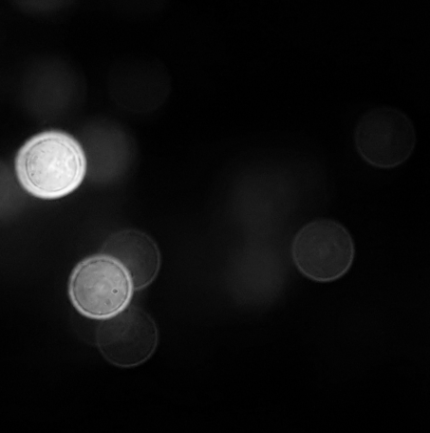
\includegraphics[width=0.25\textwidth]{warping-1-2a.png}}
%		\hfill
		\subcaptionbox{Объект за областью резкости}{%
			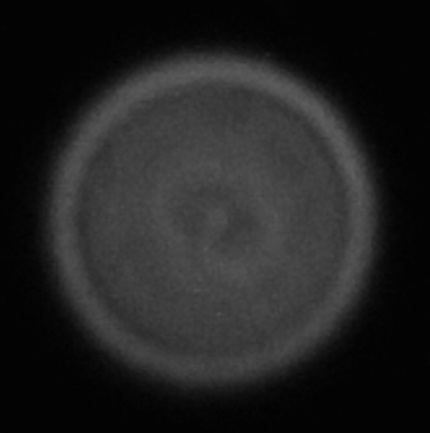
\includegraphics[width=0.25\textwidth]{warping-1-2b.png}}
		\hfill
		\subcaptionbox{Объект перед областью резкости}{%
			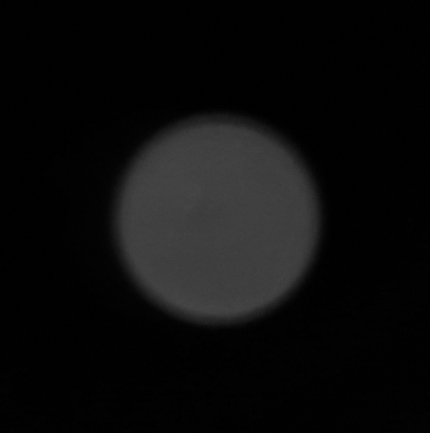
\includegraphics[width=0.25\textwidth]{warping-1-2c.png}}
		\hfill
	}
	\caption{Примеры эффекта расфокусировки}
	\label{fig:warping-defocus}
\end{figure}

Ниже приведёно описание использованных в ходе исследования моделей ядер размытия:
\begin{enumerate}[beginpenalty=10000]
	\item Ядро Гаусса.
	Задаётся формулой
	$$f_\sigma\left(x,y\right) = \frac{1}{2\pi\sigma^2}\exp\left(-\frac{x^2+y^2}{2\sigma^2}\right).$$
	Радиусом этого ядра будет считаться величина $3\sigma$.
	
	\item Круг.
	Задаётся формулой $$f_r\left(x,y\right) = \begin{cases}
		1, & x^2 + y^2 \leq r^2, \\
		0, & \text{иначе}.
	\end{cases}$$ Радиус ядра "--- радиус круга $r$.
	
	\item Круг с кольцом.
	Задаётся формулой $$f_r(x, y) = \begin{cases}
		0.25, & x^2 + y^2 \leq 0.75 r^2,\\
		1, & 0.75 r^2 < x^2 + y^2 \leq r^2,\\
		0, & \text{иначе}.
	\end{cases}$$ Радиус ядра "--- радиус круга $r$.
\end{enumerate}

Примеры этих ядер представлены на Рис.~\ref{fig:warping-psf-examples}. 

\begin{figure}[ht]
	\centerfloat{
		\hfill
		\subcaptionbox[List-of-Figures entry]{Гауссово ядро (Г)}{%
			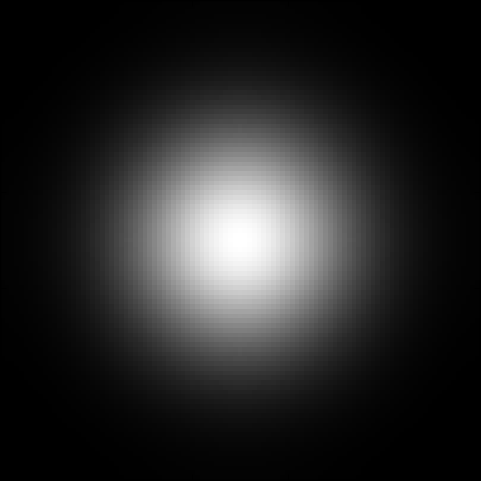
\includegraphics[width=0.25\textwidth]{warping-1-3a.png}}
		\hfill
		\subcaptionbox{Круг (К)}{%
			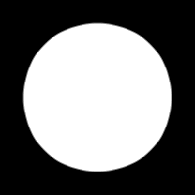
\includegraphics[width=0.25\textwidth]{warping-1-3b.png}}
		\hfill
		\subcaptionbox{Круг с кольцом (КЦ)}{%
			\includegraphics[width=0.25\textwidth]{warping-1-3c.png}}
		\hfill
	}
	\caption{Рассматриваемые ядра размытия}
	\label{fig:warping-psf-examples}
\end{figure}

\section{Построение тестового набора изображений}

Для разработки метода повышения резкости использовался набор из 24 естественных изображений из базы TID2008~\cite{ponomarenko2009tid2008}, которая является одним из стандартных наборов данных для тестирования методов обработки изображений.

При построении тестового набора к каждому изображению применялся оператор свёртки с каждым из трёх ядер размытия с разным радиусом ядра. Для круга и круга с кольцом радиус ядра размытия изменялся в пределах от 1.5 до 5 пикселей с шагом 0.5 пикселя. Для гауссова ядра "--- в пределах от 2.25 до 7.5 с шагом 0.75, что соответствует изменениям параметра $\sigma$ в пределах от 0.75 до 2.5 с шагом 0.25.

В результате для каждого типа размытия был сформирован набор из 192 изображений.

\section{Деформационный метод повышения резкости изображений}

В процессе работы алгоритма на изображении:
\begin{enumerate}[beginpenalty=10000]
	\item обнаруживаются контуры алгоритмом Кэнни~\cite{canny1986computational},
	\item производится расчёт векторов смещения пикселей в окрестности контуров,
	\item в соответствии с вычисленным векторным полем смещений деформируется пиксельная сетка,
	\item полученный результат проецируется на регулярную сетку выходного изображения с помощью интерполяции, описанной в~\cite{krylov2014gridwarping}.
\end{enumerate}

Направление и величина смещения пикселей задаётся функцией смещения $d\left(x\right)$, $x_{new} \leftarrow x_{old}+d(x_{old})$. В одномерном случае, если центр контура находится в точке $x = 0$, вектора смещения определяются функцией близости $p\left(x\right)=1+d^{\,\prime}(x)$.

Она может быть выражена через p(x) с помощью уравнения

\begin{equation*}
	d\left(x\right)=\int_{-\infty}^{x}\left(p\left(y\right)-1\right)dy.
\end{equation*}

Функция $p(x)$ выражает расстояние между соседними пикселями изображения: если её значение меньше 1, в точке $x$ уплотнение; если больше 1 "--- разрежение. Для недеформированных изображений $p(x)\equiv1$.

Чтобы взаимное расположение точек при смещении не менялось, для функции $d(x)$ должно быть выполнено $x_1<x_2 \Rightarrow x_1+d(x_1)\le x_2+d(x_2)$. Отсюда получаем ограничение $d^{\,\prime}\left(x\right)\geq-1$. Также деформироваться должна только сетка вблизи контуров, поэтому $d\left(x\right)\rightarrow0$ при  $\left|x\right|\rightarrow\infty$. Пример функции близости приведён на Рис.~\ref{fig:warping-proximity}.

\begin{figure}[ht]
	\centerfloat{
		\includegraphics[height=0.4\textheight]{warping-1-5.png}
	}
	\caption{Пример функции близости и результата смещения пикселей с её помощью}
	\label{fig:warping-proximity}
\end{figure}

В двумерном случае смещение задаётся векторным полем $\vec{d}(x,y)$, которое удовлетворяет уравнению $p\left(x,y\right)=1+div\,\vec{d}(x,y)$. Помимо этого, во избежание возникновения завихрений требуется ограничение $rot\, \vec{d}=0$, а так как $rot\, \nabla u \equiv 0$, то, если функция $p(x, y)$ известна, векторное поле смещений можно представить как $\vec{d}\left(x,y\right)=\nabla u\left(x,y\right)$, где функция $u\left(x,y\right)$ является решением уравнения

\begin{equation*}
	\left\{
		\begin{aligned}
			&\Delta u = p\left(x,y\right) - 1, \\
			&u\mid_\Gamma=0,
		\end{aligned}
	\right.
\end{equation*}

\noindent где $\Gamma$ "--- граница изображения.

В работе~\cite{gusev2016parallel} предлагается для двумерного случая использовать функцию близости одной переменной для построения функции близости на плоскости:

\begin{align*}
	&p\left(x,y\right) = \frac{\sum_{\left(x_e,y_e\right) \in N\left(x,y\right)}{w\left(x_e,y_e\right)p\left(x_n\right)}} {\sum_{\left(x_e,y_e\right) \in N\left(x,y\right)}{w\left(x_e,y_e\right)}}, \\
	&w\left(x_e,y_e\right) = G_{\sigma}\left(x_t\right)\lvert \vec{g}\left(x_e,y_e\right) \rvert,
\end{align*}

\noindent где $N\left(x,y\right)$ "--- это множество соседних точек вокруг т.~$\left(x, y\right)$; $x_n$ и $x_t$ "--- это проекции вектора $\left(x-x_e, y-y_e\right)$ на вектор градиента изображения $\vec{g}\left(x_e,y_e\right)$ и на нормаль к нему соответственно; а $G_{\sigma}\left(x_t\right) = \frac{1}{\sigma \sqrt{2\pi}} \exp\left(\frac{-x^2}{2\sigma^2}\right)$.

В этом случае итоговая функция смещения имеет следующий вид~\cite{gusev2016parallel}:

\begin{equation*}
	\vec{d}\left(x,y\right) = \frac{\sum_{\left(x_e,y_e\right) \in N\left(x,y\right)}{d\left(x_n\right) G_{\sigma}\left(x_t\right) \vec{g}\left(x_e,y_e\right) }} {\sum_{\left(x_e,y_e\right) \in N\left(x,y\right)}{G_{\sigma}\left(x_t\right)\lvert \vec{g}\left(x_e,y_e\right) \rvert}}.
\end{equation*}

Таким образом, можно перейти к работе с функцией смещения напрямую и проанализировать её влияние на результаты работы деформационного алгоритма повышения резкости.

\section{Модели функции смещения}

Были рассмотрены три модели функции смещения, первая из которых была предложена в оригинальной работе авторов метода и используется здесь для оценки повышения эффективности деформационного метода повышения резкости изображений:
\begin{enumerate}[beginpenalty=10000]
	\item $d_0\left(x;\sigma\right)=\sigma\sqrt\pi\left[erf\left(\frac{x}{2\sigma}\right)-erf\left(\frac{x}{\sigma}\right)\right]$, где $erf{\left(x\right)}=\frac{2}{\sqrt\pi}\int_{0}^{x}{e^{-t^2}dt}$;
	\item
	$
	\begin{aligned}
		d_2\left(x;a,b,c\right)=\left\{
		\begin{aligned}
			&\frac{c}{a}x,\ \left|x\right|<a,\\
			&c\frac{b-\left|x\right|}{b-a} \cdot sign\left(x\right),\ a\le\left|x\right|<b,\\
			&0,\ \left|x\right|\geq b;
		\end{aligned}
		\right.
	\end{aligned}
	$
	\item $d_1(x;a,c)$, имеющая тот же вид, что и $d_2(x)$, но $b=1.5a$.
\end{enumerate}

При этом координата $x$ "--- это расстояние точки от контура, делённое на радиус ядра размытия, что позволяет масштабировать функцию для разных уровней размытия без изменения самих параметров $a$, $b$, $c$ и $\sigma$.

Пример функции $d_2(x;a,b,c)$ приведёт на Рис.~\ref{fig:warping-d2-example}.

\begin{figure}[ht]
	\centerfloat{
		\includegraphics[width=0.4\textwidth]{warping-1-6.png}
	}
	\caption{Вид функции смещения $d_2(x;a,b,c)$}
	\label{fig:warping-d2-example}
\end{figure}

\section{Методика оптимизации параметров моделей функций смещения}

Проводился поиск оптимальных параметров рассматриваемых малопараметрических (одно"~ и двухпараметрических) моделей функций смещения для разных типов размытия, а затем "--- сравнительный анализ результатов обработки размытых изображений деформационным методом повышения резкости с использованием полученных результатов.

%Для нахождения оптимальных параметров проводилась минимизация среднего значения показателя RMSE по всем изображениям для одного типа размытия:

%\begin{align*}
%	\frac{1}{\left|V\right|}\sum_{V}{RMSE(u,v)\rightarrow \min_{z}}, \quad
%	RMSE\left(u,v\right)=\sqrt{\frac{1}{WH}\sum_{i,j}{(u_{ij}-v_{ij})}^2}.
%\end{align*}

Для нахождения оптимальных параметров проводилась минимизация среднего значения показателя MSE по всем изображениям для одного типа размытия:

\begin{align*}
	\frac{1}{\left|V\right|}\sum_{V}{MSE\left(u,v\right) \rightarrow \min_{z}}, \quad
	MSE\left(u,v\right)=\frac{1}{WH}\sum_{i,j}{(u_{ij}-v_{ij})}^2,
\end{align*}

\noindent а в качестве показателя качества "--- значение $PSNR\left(u,v\right) = 10 \cdot \log_{10}{\left(\frac{255^2}{MSE\left(u,v\right)}\right)}$.

Здесь $v$ "--- размытое изображение, обработанное методом повышения резкости, $u$ "--- соответствующее ему истинное резкое изображение, $V$ "--- множество всех размытых изображений для одного ядра размытия, $W$ и $H$ "--- ширина и высота изображения в пикселях соответственно, $z$ "--- соответствующие рассматриваемой функции смещения параметры из множества $\left\{a, b, c, \sigma\right\}$.

Для решения задачи минимизации применялся метод Нелдера"=Мида~\cite{10.1093/comjnl/7.4.308}. Число итераций было ограничено числом 100, минимальный шаг был установлен в $10^{-3}$. С начальным приближением $a=1$, $b=1.5$, $c=0.5$, $\sigma=1$ процесс оптимизации завершился примерно на 50-й итерации. Было сделано несколько запусков процесса оптимизации с разными начальными приближениями для достижения глобального оптимума.

\section{Результаты экспериментов}

В ходе экспериментов было установлено, что наилучшие результаты достигаются при $a=-c$. Такое соотношение параметров обеспечивает наибольшее смещение пикселей в районе контура без нарушения ограничения на производную функции смещения. Поэтому в дальнейшем это соотношение всегда выполняется, что позволяет перейти к модели с двумя (функция $d_2(x;a,b,c=-a)$) и одним (функция $d_1(x;a,c=-a)$) параметрами.

После проведения исследования и поиска оптимальных параметров функций смещения для каждого типа размытия были получены следующие результаты. Условные обозначения типов ядер размытия: Г "--- гауссово ядро, К "--- круг, КЦ "--- круг с кольцом.

%На Рис.~\ref{fig:warping-best-displacements} представлены функции смещения, оптимальные только для своего типа размытия. Красным цветом отмечена модель с двумя параметрами (с функцией $d_2\left(x\right)$), а синим "--- модель с одним параметром  (с функцией $d_1\left(x\right)$). Условные обозначения типов ядер размытия: Г "--- гауссово ядро, К "--- круг, КЦ "--- круг с кольцом.

%\begin{figure}[ht]
%	\centerfloat{
%		\includegraphics[width=0.9\textwidth]{warping-1-7.png}
%	}
%	\caption{Функция смещения для моделей с 1 и 2 параметрами}
%	\label{fig:warping-best-displacements}
%\end{figure}

%Усреднённые по набору изображений значения RMSE входных размытых и обработанных изображений для функций смещения $d_0\left(x\right)$ и $d_2\left(x\right)$ с оптимальными параметрами приведены в Табл.~\ref{tab:warping-rmse-d0-d2}. Из неё видно, что предложенная функция $d_2\left(x\right)$ позволяет достичь более качественного результата.

%\begin{table} [htbp]%
%%	\tiny
%	\small
%	\centering
%	\caption{Средние значения RMSE размытых и обработанных изображений для функций смещения $d_0\left(x\right)$ и $d_2\left(x\right)$ (сила размытия обозначена номером радиуса размытия в порядке возрастания)}%
%	\label{tab:warping-rmse-d0-d2}% label всегда желательно идти после caption
%	\renewcommand{\arraystretch}{1.5}%% Увеличение расстояния между рядами, для улучшения восприятия.
%	\begin{SingleSpace}
%		\begin{tabulary}{\textwidth}{@{}@{\extracolsep{5pt}}cCCCCCCCCC@{}} %Вертикальные полосы не используются принципиально, как и лишние горизонтальные (допускается по ГОСТ 2.105 пункт 4.4.5) % @{} позволяет прижиматься к краям
%			\toprule     %%% верхняя линейка
%			& \multicolumn{3}{@{}c@{}}{\makecell{Размытые \\ изображения}} & \multicolumn{3}{@{}c@{}}{\makecell{$d_0\left(x\right)$}} & \multicolumn{3}{@{}c@{}}{\makecell{$d_2\left(x\right)$}} \\
%			\cmidrule(r){2-4}\cmidrule(lr){5-7}\cmidrule(l){8-10}
%			\makecell{Сила \\ размытия}  &  Г & К & КЦ  &  Г & К & КЦ  &  Г & К & КЦ \\
%			\midrule %%% тонкий разделитель. Отделяет названия столбцов. Обязателен по ГОСТ 2.105 пункт 4.4.5
%			1 & 13.470 & 9.750 & 11.004 & 13.119 & 9.603 & 10.794 & 13.015 & 9.516 & 10.620 \\
%			2 & 15.481 & 11.849 & 13.525 & 15.039 & 11.585 & 13.176 & 14.912 & 11.492 & 12.974 \\
%			3 & 16.905 & 13.869 & 15.446 & 16.385 & 13.483 & 14.980 & 16.260 & 13.365 & 14.750 \\
%			4 & 18.037 & 14.975 & 16.383 & 17.489 & 14.558 & 15.898 & 17.370 & 14.455 & 15.710 \\
%			5 & 18.951 & 16.093 & 17.488 & 18.386 & 15.622 & 16.954 & 18.274 & 15.525 & 16.782 \\
%			6 & 19.749 & 16.893 & 18.255 & 19.169 & 16.412 & 17.712 & 19.063 & 16.327 & 17.563 \\
%			7 & 20.437 & 17.625 & 18.973 & 19.836 & 17.120 & 18.405 & 19.730 & 17.044 & 18.273 \\
%			8 & 21.070 & 18.270 & 19.599 & 20.462 & 17.761 & 19.027 & 20.352 & 17.693 & 18.905 \\
%			\midrule
%			Среднее & 18.013 & 14.916 & 16.334 & 17.486 & 14.518 & 15.868 & 17.372 & 14.427 & 15.697 \\
%			\bottomrule %%% нижняя линейка
%		\end{tabulary}%
%	\end{SingleSpace}
%\end{table}

Усреднённые по набору изображений значения PSNR входных размытых и обработанных изображений для функций смещения $d_0\left(x\right)$ и $d_2\left(x\right)$ с оптимальными параметрами приведены в Табл.~\ref{tab:warping-psnr-d0-d2}. Из неё видно, что предложенная функция $d_2\left(x\right)$ позволяет достичь более качественного результата.

\begin{table} [htbp]%
	%	\tiny
	\small
	\centering
	\caption{Средние значения PSNR размытых и обработанных изображений для функций смещения $d_0\left(x\right)$ и $d_2\left(x\right)$ (сила размытия обозначена номером радиуса размытия в порядке возрастания)}%
	\label{tab:warping-psnr-d0-d2}% label всегда желательно идти после caption
	\renewcommand{\arraystretch}{1.5}%% Увеличение расстояния между рядами, для улучшения восприятия.
	\begin{SingleSpace}
		\begin{tabulary}{\textwidth}{@{}@{\extracolsep{5pt}}cCCCCCCCCC@{}} %Вертикальные полосы не используются принципиально, как и лишние горизонтальные (допускается по ГОСТ 2.105 пункт 4.4.5) % @{} позволяет прижиматься к краям
			\toprule     %%% верхняя линейка
			& \multicolumn{3}{@{}c@{}}{\makecell{Размытые \\ изображения}} & \multicolumn{3}{@{}c@{}}{\makecell{$d_0\left(x\right)$}} & \multicolumn{3}{@{}c@{}}{\makecell{$d_2\left(x\right)$}} \\
			\cmidrule(r){2-4}\cmidrule(lr){5-7}\cmidrule(l){8-10}
			\makecell{Сила \\ размытия}  &  Г & К & КЦ  &  Г & К & КЦ  &  Г & К & КЦ \\
			\midrule %%% тонкий разделитель. Отделяет названия столбцов. Обязателен по ГОСТ 2.105 пункт 4.4.5
			1	& 25.543	& 28.351	& 27.300	& 25.773	& 28.483	& 27.468	& 25.842	& 28.561	& 27.608 \\
			2	& 24.335	& 26.657	& 25.508	& 24.587	& 26.853	& 25.735	& 24.660	& 26.923	& 25.870 \\
			3	& 23.571	& 25.290	& 24.355	& 23.842	& 25.535	& 24.621	& 23.908	& 25.612	& 24.755 \\
			4	& 23.008	& 24.623	& 23.843	& 23.276	& 24.869	& 24.104	& 23.335	& 24.930	& 24.207 \\
			5	& 22.578	& 23.998	& 23.276	& 22.841	& 24.256	& 23.546	& 22.894	& 24.310	& 23.634 \\
			6	& 22.220	& 23.577	& 22.903	& 22.478	& 23.827	& 23.165	& 22.527	& 23.873	& 23.239 \\
			7	& 21.922	& 23.208	& 22.568	& 22.182	& 23.461	& 22.832	& 22.228	& 23.499	& 22.895 \\
			8	& 21.658	& 22.896	& 22.286	& 21.912	& 23.141	& 22.543	& 21.959	& 23.175	& 22.599 \\
			\midrule
			Среднее	& 23.104	& 24.825	& 24.005	& 23.361	& 25.053	& 24.252	& 23.419	& 25.110	& 24.351  \\
			\bottomrule %%% нижняя линейка
		\end{tabulary}%
	\end{SingleSpace}
\end{table}

%В Табл.~\ref{tab:warping-rmse-d1} представлены показатели снижения RMSE относительно размытых изображений для вариантов алгоритма на основе функции смещения с 2 и с 1 параметром. Модуль относительной разницы не превышает 4\%, а в среднем равен 1.2\%, что позволяет говорить о сравнимом качестве работы обоих вариантов метода и возможности использовать однопараметрический вариант без значительных потерь в качестве.
%
%\begin{table} [htbp]%
%	\centering
%	\caption{Средние значения снижения RMSE для изображений, обработанных с использованием функции смещения $d_2\left(x\right)$ и $d_1\left(x\right)$, по сравнению с размытыми изображениями}%
%	\label{tab:warping-rmse-d1}% label всегда желательно идти после caption
%	\renewcommand{\arraystretch}{1.5}%% Увеличение расстояния между рядами, для улучшения восприятия.
%	\begin{SingleSpace}
%		\begin{tabulary}{\textwidth}{@{}@{\extracolsep{10pt}}cCCCCCC@{}} %Вертикальные полосы не используются принципиально, как и лишние горизонтальные (допускается по ГОСТ 2.105 пункт 4.4.5) % @{} позволяет прижиматься к краям
%			\toprule     %%% верхняя линейка
%			& \multicolumn{3}{@{}c@{}}{\makecell{$d_2\left(x\right)$}} & \multicolumn{3}{@{}c@{}}{\makecell{$d_1\left(x\right)$}} \\
%			\cmidrule(r){2-4}\cmidrule(l){5-7}
%			\makecell{Сила \\ размытия}  &  Г & К & КЦ  &  Г & К & КЦ \\
%			\midrule %%% тонкий разделитель. Отделяет названия столбцов. Обязателен по ГОСТ 2.105 пункт 4.4.5
%			1 & 0.455 & 0.234 & 0.384 & 0.456 & 0.227 & 0.399 \\
%			2 & 0.569 & 0.357 & 0.551 & 0.569 & 0.365 & 0.551 \\
%			3 & 0.645 & 0.504 & 0.696 & 0.645 & 0.508 & 0.671 \\
%			4 & 0.667 & 0.520 & 0.673 & 0.666 & 0.518 & 0.654 \\
%			5 & 0.677 & 0.568 & 0.706 & 0.677 & 0.563 & 0.693 \\
%			6 & 0.686 & 0.566 & 0.692 & 0.686 & 0.56 & 0.682 \\
%			7 & 0.707 & 0.581 & 0.700 & 0.708 & 0.578 & 0.687 \\
%			8 & 0.718 & 0.577 & 0.694 & 0.718 & 0.575 & 0.676 \\
%			\midrule
%			Среднее & 0.641 & 0.489 & 0.637 & 0.641 & 0.487 & 0.627 \\
%			\bottomrule %%% нижняя линейка
%		\end{tabulary}%
%	\end{SingleSpace}
%\end{table}

В Табл.~\ref{tab:warping-psnr-d1} представлены показатели среднего прироста PSNR (ISNR) относительно размытых изображений для вариантов алгоритма на основе функции смещения с 2 и с 1 параметром. Модуль относительной разницы не превышает 4.2\%, а в среднем равен 1.1\%, что позволяет говорить о сравнимом качестве работы обоих вариантов метода и возможности использовать однопараметрический вариант без значительных потерь в качестве.
Оптимальные значения параметра $a$ однопараметрического метода с функцией $d_1\left(x\right)$ для гауссовского ядра размытия, ядра типа "круг" и ядра типа "круг с кольцом" составили $1.28$, $1.12$ и $1.16$ соответственно.

\begin{table} [htbp]%
	\centering
	\caption{Средние значения прироста PSNR для изображений, обработанных с использованием функции смещения $d_2\left(x\right)$ и $d_1\left(x\right)$, по сравнению с размытыми изображениями}%
	\label{tab:warping-psnr-d1}% label всегда желательно идти после caption
	\renewcommand{\arraystretch}{1.5}%% Увеличение расстояния между рядами, для улучшения восприятия.
	\begin{SingleSpace}
		\begin{tabulary}{\textwidth}{@{}@{\extracolsep{10pt}}cCCCCCC@{}} %Вертикальные полосы не используются принципиально, как и лишние горизонтальные (допускается по ГОСТ 2.105 пункт 4.4.5) % @{} позволяет прижиматься к краям
			\toprule     %%% верхняя линейка
			& \multicolumn{3}{@{}c@{}}{\makecell{$d_2\left(x\right)$}} & \multicolumn{3}{@{}c@{}}{\makecell{$d_1\left(x\right)$}} \\
			\cmidrule(r){2-4}\cmidrule(l){5-7}
			\makecell{Сила \\ размытия}  &  Г & К & КЦ  &  Г & К & КЦ \\
			\midrule %%% тонкий разделитель. Отделяет названия столбцов. Обязателен по ГОСТ 2.105 пункт 4.4.5
			1	& 0.299	& 0.210	& 0.308	& 0.299	& 0.204	& 0.321 \\
			2	& 0.325	& 0.266	& 0.362	& 0.325	& 0.272	& 0.361 \\
			3	& 0.337	& 0.322	& 0.400	& 0.337	& 0.324	& 0.386 \\
			4	& 0.327	& 0.307	& 0.364	& 0.327	& 0.306	& 0.354 \\
			5	& 0.316	& 0.312	& 0.358	& 0.316	& 0.309	& 0.351 \\
			6	& 0.307	& 0.296	& 0.336	& 0.307	& 0.293	& 0.331 \\
			7	& 0.306	& 0.291	& 0.327	& 0.306	& 0.290	& 0.321 \\
			8	& 0.301	& 0.279	& 0.313	& 0.301	& 0.278	& 0.305 \\
			\midrule
			Среднее	& 0.315	& 0.285	& 0.346	& 0.315	& 0.285	& 0.341 \\
			\bottomrule %%% нижняя линейка
		\end{tabulary}%
	\end{SingleSpace}
\end{table}

%Из Рис.~\ref{fig:warping-best-displacements} видно, что для разных типов ядер размытия относительные значения оптимальных параметров функций смещения близки.
Дополнительный анализ изменения среднего прироста показателя PSNR показал, что при несильном отклонении параметра от оптимального значения качество результирующего изображения снижается слабо (см. Рис.~\ref{fig:warping-isnr-change}).

\begin{figure}[ht]
	\centerfloat{
		\includegraphics[width=0.8\textwidth]{warping-1-extra1.png}
	}
	\caption{Изменение прироста показателя PSNR при относительном изменении параметра $a$}
	\label{fig:warping-isnr-change}
\end{figure}

На Рис.~\ref{fig:warping-eye}~и~\ref{fig:warping-eye2} приведены примеры результата обработки медицинского изображения полученным методом. Видно повышение резкости контуров сосудов и диска зрительного нерва.

\begin{figure}[ht]
	\centerfloat{
		\hfill
		\subcaptionbox[List-of-Figures entry]{Входное изображение}{%
			\includegraphics[height=0.3\textheight]{warping-1-8a.png}}
		\hfill
		\subcaptionbox{Обработанное изображение}{%
			\includegraphics[height=0.3\textheight]{warping-1-8b.png}}
		\hfill
	}
	\caption{Применение деформационного алгоритма с использованием функции смещения $d_1\left(x\right)$ как шага постобработки в задаче повышения разрешения медицинских изображений}
	\label{fig:warping-eye}
\end{figure}

\begin{figure}[ht]
	\centerfloat{
		\hfill
		\subcaptionbox[List-of-Figures entry]{Входное изображение}{%
			\includegraphics[height=0.25\textheight]{warping-1-extra2a.png}}
		\hfill
		\subcaptionbox{Обработанное изображение}{%
			\includegraphics[height=0.25\textheight]{warping-1-extra2b.png}}
		\hfill
	}
	\caption{Применение деформационного алгоритма с использованием функции смещения $d_1\left(x\right)$ как шага постобработки в задаче повышения разрешения медицинских изображений}
	\label{fig:warping-eye2}
\end{figure}

\section{Выводы} 

%Предложенные функции смещения $d_2\left(x\right)$ и $d_1\left(x\right)$ демонстрируют улучшение качества обработки изображений по сравнению с оригинальной функцией $d_0\left(x\right)$, выражаемое в приросте снижения показателя RMSE, в среднем на 30\%. Вариант алгоритма на основе однопараметрической функция смещения $d_1\left(x\right)$ почти не отличается от двухпараметрического варианта качеством результатов, благодаря этому можно использовать его для всех трёх рассмотренных ядер размытия.

Предложенные функции смещения $d_2\left(x\right)$ и $d_1\left(x\right)$ демонстрируют улучшение качества обработки изображений по сравнению с оригинальной функцией $d_0\left(x\right)$, выражаемое в приросте показателя PNSR, в среднем на 27\%. Вариант алгоритма на основе однопараметрической функция смещения $d_1\left(x\right)$ почти не отличается от двухпараметрического варианта качеством результатов, благодаря этому можно использовать его для всех трёх рассмотренных ядер размытия.

\FloatBarrier
           % Глава 2
\chapter{Нейросетевой алгоритм контроля качества рентгеновских снимков грудной клетки в задаче диагностики туберкулёза лёгких}\label{ch:ch3}

Согласно клиническим рекомендациям Минздрава России, одним из первых этапов выявления и диагностики туберкулёза лёгких является рентгенофлюорографическое исследование~\cite{васильева2022туберкулез}. При этом в последние годы в практику внедряются компьютерные системы автоматической обработки медицинских данных и диагностики заболеваний на основе искуственного интеллекта, в том числе для в категории флюорографии~\cite{СМ106054, рг2023, рбк2023, интерфакс2023}.

Одной из актуальных задач при применении методов глубокого обучения в медицинской диагностике является анализ и предобработка входных данных. Необходим контроль соответствия входной информации и применяемого обученного (обучаемого) метода глубокого обучения. Это, например, требуется при контроле наличия адверсативных атак на данные~\cite{finlayson2019adversarial}.

Контроль качества рентгеновских снимков грудной клетки на основании разных параметров важен для полноценного анализа снимка и постановки правильного диагноза. Автоматическое определение контроля пространственных условий снимка (позы пациента, положения грудной клетки в кадре и т.п.) рассматривается в работах~\cite{nousiainen2021automating, von2020robust, jia2019application}. В работе~\cite{sadre2021validating} изучено влияние качества снимка на результаты автоматической диагностики COVID"~19.

В данной главе контроль входных рентгеновских снимков используется для проверки соответствия уровня облучения снимка уровню, требуемому для качественной диагностики туберкулёза лёгких. Рассматриваются:
\begin{enumerate}[beginpenalty=10000]
	\item задача автоматического определения уровня жёсткости рентгеновского снимка грудной клетки с помощью нейросетевого алгоритма;
	\item влияние предварительной фильтрации обучающей и валидационной выборок на качество работы алгоритма классификации в задаче диагностики туберкулёза лёгких по рентгеновским снимкам грудной клетки.
\end{enumerate}

Несмотря на то, что использование при анализе рентгенограммы грудной клетки, помимо фронтальной, также и боковой проекции повышает качество анализа, в том числе компьютерного, прирост качества для разных задач разный и далеко не всегда значительный~\cite{kluthke2016additional, hashir2020quantifying}. Кроме того, на практике в подавляющем числе случаев имеются только снимки, сделанные во фронтальной проекции~\cite{вишнякова2016частота}, поэтому в рамках данной главы рассматриваются фронтальные изображения грудной клетки.

\section{Метод оценки жёсткости рентгеновских снимков грудной клетки}

При изучении рентгеновских снимков грудной клетки, и в частности при диагностике туберкулёза лёгких, важным фактором является жёсткость снимка, так как она напрямую влияет на его информативность~\cite{chuiko1982effects, тимофеева2013основные}. Уровень жёсткости обусловлен дозой радиации, длиной волны излучения и особенностями тела пациента. При условии правильного контрастирования снимка уровень жёсткости можно определить визуально, подсчитав число отчётливо видимых на снимке верхних грудных позвонков: оптимальному уровню в задаче диагностики туберкулёза лёгких соответствуют 3"~4 видимых позвонка, а меньшее или большее число свидетельствует о том, что снимок слишком мягкий или жёсткий~\cite{тимофеева2013основные, сидоров2012методика}. Пример рентгеновского изображения позвоночного столба с указанием номеров позвонков приведён на Рис.~\ref{fig:vertebral-column}, а примеры снимков разного уровня жёсткости представлены на Рис.~\ref{fig:samples-different-hardness}.

\begin{figure}[ht]
	\centerfloat{
		\includegraphics[height=0.3\textheight]{example_vertebrae.png}
	}
	\caption{Пример рентгеновского изображения позвоночника с номерами шейных (C) и грудных (T) позвонков}
	\label{fig:vertebral-column}
\end{figure}

\begin{figure}[ht]
	\centerfloat{
		\hfill
		\subcaptionbox[List-of-Figures entry]{Мягкий снимок}{%
			\includegraphics[width=0.3\textwidth]{example_soft.png}}
		\hfill
		\subcaptionbox{Нормальный снимок}{%
			\includegraphics[width=0.3\textwidth]{example_normal.png}}
		\hfill
		\subcaptionbox{Жёсткий снимок}{%
			\includegraphics[width=0.3\textwidth]{example_hard.png}}
		\hfill
	}
	\caption{Примеры рентгеновских снимков грудной клетки разной жёсткости}
	\label{fig:samples-different-hardness}
\end{figure}

Настоящее исследование развивает идеи работы \cite{dovganich2022automatic}, где было показано, что оптимизация алгоритма диагностики заболеваний по рентгеновскому снимку грудной клетки для работы с изображениями близкой жёсткости вместе с автоматическим контролем качества рентгеновских изображений позволяет достичь точности классификации выше, чем у алгоритма, созданного в расчёте на обработку разнородных по уровню жёсткости изображений. В ходе выполнения данного исследования был применён полностью нейросетевой подход.

Предлагаемый метод оценки жёсткости включает 2 этапа: обучение и применение. В процессе обучения нейросетевая модель, являющаяся основой метода, однократно настраивается с целью оптимального решения задачи и сохраняется для дальнейшего использования. На этапе применения происходит непосредственный анализ изображений.

Процесс обучения выглядит следующим образом:
\begin{enumerate}[beginpenalty=10000]
	\item предобработка входных данных;
	\item итеративный процесс минимизации функции потерь (функционала, отображающего выходные значения нейросетевой модели в показатель их близости к оптимальным значениям для решения задачи) повторением шагов:
	\begin{enumerate}[beginpenalty=10000]
		\item подача предобработанных выходных данных на вход нейросетевой модели и получение её выходных значений;
		\item получение значения функции потерь для данных выходных значений модели и входных данных;
		\item шаг оптимизации;
		\item замер качества работы алгоритма;
		\item проверка условия ранней остановки процесса минимизации;
	\end{enumerate}
	\item сохранение модели.	
\end{enumerate}

Процесс применения метода состоит из следующих шагов:
\begin{enumerate}[beginpenalty=10000]
	\item предобработка входных данных;
	\item подача предобработанных выходных данных на вход нейросетевой модели и получение её выходных значений.
\end{enumerate}

\subsection{Использованные данные}

При решении рассматриваемой задачи были использованы 2 набора рентгенограмм грудной клетки, снятых во фронтальной проекции.

Первый набор изображений был собран в сотрудничестве с медиками из НПЦ~<<Фтизиатрия>> им. Е.Н.~Андреева в г. Якутск и применялся для обучения нейросетевой модели для метода определения жёсткости рентгенограмм.

Второй набор был сформирован из двух наиболее часто используемых при разработке методов компьютерной диагностики туберкулёза лёгких общедоступных наборов рентгенограмм, ставших, можно сказать, эталонными~\cite{oloko2022systematic, zeyu2022review, singh2022evolution, santosh2022advances}: Montgomery County~\cite{candemir2013lung} и Shenzhen~\cite{jaeger2013automatic}. Так как в большинстве работ наборы Montgomery County и Shenzhen используются вместе~\cite{oloko2022systematic, zeyu2022review}, то было принято решение их объединить и обозначать <<Montgomery"~Shenzhen>> (MC"~SZ). Полученный набор снимков использовался для оценки качества работы разработанного алгоритма на снимках, сделанных в других медицинских учреждениях, на другом оборудовании и при других условиях.

\subsubsection{Набор рентгенограмм грудной клетки SakhaTB} \label{subsubsec:dataset-yak-hardness}

Набор состоит из 1298 рентгеновских снимков грудной клетки больных туберкулёзом лёгких пациентов, собранных в нескольких медицинских учреждениях Республики Саха (Якутия) при помощи стационарных и переносных комплексов оборудования. Разрешение изображений разнится  и находится в диапазоне примерно от 2000x2000 до 3000x3000 пикселей. Большинство рентгенограмм имеет глубину цвета 16 бит, у остальных снимков она равна 8 битам.

Для дальнейшей работы глубина цвета снимков предварительно была приведена к 8 битам, а разрешение путём усреднения соседних пикселей было уменьшено в целое число раз до достижения значений около 1000x1000. Одновременно была проведена нормализация диапазона интенсивности пикселей с отсечением (англ.~clipping) по 0.5\% пикселей с каждого конца гистограммы изображения и обрезкой по 1.5\% пикселей с каждой стороны изображений, чтобы увеличить долю диапазона допустимых значений 8 бит информации, приходящуюся на внутренние органы грудной клетки. Примеры снимков приведены на Рис.~\ref{fig:samples-yak-hardness}.

Подмножество снимков этого набора было выложено вместе с рентгенограммами грудной клетки здоровых пациентов для использования в открытый доступ под названием Sakha"~TB (см.~п.~\ref{sec:sakha-tb}).

\begin{figure}[ht]
	\centerfloat{
    	\includegraphics[width=0.9\textwidth]{sakhatb.png}
	}
	\caption{Примеры изображений из набора SakhaTB}
	\label{fig:samples-yak-hardness}
\end{figure}

%\subsubsection{Набор Montgomery County} \label{subsubsec:dataset-mc}

\subsubsection{Набор рентгенограмм грудной клетки Montgomery"~Shenzhen} \label{subsubsec:dataset-mc-sz}

Набор изображений Montgomery County (далее MC) предоставляется Национальной библиотекой медицины Национальных институтов здравоохранения США и собран Министерством здравоохранения и социальных служб США в округе Монтгомери штата Мэриленд. Он содержит рентгеновские снимки грудной клетки в оттенках серого с глубиной цвета 8 бит в формате PNG с разрешением 4020x4892 пикселей и их метки соответствия 2 классам: 80 рентгенограмм здоровых и 58 рентгенограмм больных туберкулёзом лёгких пациентов. %Примеры снимков приведены на Рис.~\ref{fig:samples-mc-sz}.

%\subsubsection{Набор Shenzhen} \label{subsubsec:dataset-sz}

Набор изображений Shenzhen (далее SZ) предоставляется Национальной библиотекой медицины Национальных институтов здравоохранения США и собран Медицинским колледжем провинции Гуандун в Народном госпитале №~3 г.~Шэньчжэнь в КНР. Он содержит рентгеновские снимки грудной клетки в оттенках серого с глубиной цвета 8 бит в формате PNG с различным разрешением (примерно 3000x3000 пикселей) и их метки соответствия 2 классам: 326 рентгенограмм здоровых и 336 рентгенограмм больных туберкулёзом лёгких пациентов.

Примеры снимков объединённого набор приведены на Рис.~\ref{fig:samples-mc-sz}.

%\begin{figure}[ht]
%	\begin{minipage}[b][][b]{0.9\textwidth}\centering
%		\includegraphics[width=0.9\textwidth]{mcsz-normal.png} \\
%		{а)~Здоровые пациенты}
%	\end{minipage}
%	\hfill
%	\begin{minipage}[b][][b]{0.9\textwidth}\centering
%		\includegraphics[width=0.9\textwidth]{mcsz-tb.png} \\
%		{б)~Пациенты, больные туберкулёзом}
%	\end{minipage}
%	\caption{Примеры изображений из объединённого набора Montgomery"~Shenzhen (MC"~SZ)}
%	\label{fig:samples-mc-sz}
%\end{figure}

\begin{figure}[ht]
	\centerfloat{
%		\hfill
		\subcaptionbox[List-of-Figures entry]{Здоровые пациенты}{%
			\includegraphics[height=0.25\textheight]{mcsz-normal.png}}
%		\hfill
		\vfill
%		\hfill
		\subcaptionbox{Пациенты, больные туберкулёзом лёгких}{%
			\includegraphics[height=0.25\textheight]{mcsz-tb.png}}
%		\hfill
		\vfill
	}
	\caption{Примеры изображений из объединённого набора Montgomery"~Shenzhen (MC"~SZ)}
	\label{fig:samples-mc-sz}
\end{figure}

\subsubsection{Аннотирование данных}

Для обоих наборов (SakhaTB, собранный в рамках исследования, и MC"~SZ) была проведена процедура аннотации врачом-рентгенологом из НПЦ~<<Фтизиатрия>> им. Е.Н.~Андреева в г. Якутск. В рамках процедуры каждому изображению ставился в соответствие его уровень жёсткости, выраженный числом отчётливо видимых на этом снимке верхних грудных позвонков.  Распределение изображений по такому показателю жёсткости представлено на Рис.~\ref{fig:vertebrae-yak-hardness}"~\ref{fig:vertebrae-mc-sz}.

\begin{figure}[ht]
	\centerfloat{
		\includegraphics[height=0.3\textheight]{total_vertebrae_hist.png}
	}
	\caption{Гистограмма распределения снимков набора SakhaTB по числу отчётливо видимых позвонков}
	\label{fig:vertebrae-yak-hardness}
\end{figure}

\begin{figure}[ht]
	\centerfloat{
		\includegraphics[height=0.25\textheight]{total_vertebrae_hist_mc-sz.png}
	}
	\caption{Гистограмма распределения снимков набора MC"~SZ по числу отчётливо видимых позвонков}
	\label{fig:vertebrae-mc-sz}
\end{figure}

\subsection{Адаптивная предобработка входных изображений} \label{subsec:tb-hardness-preprocessing}

Хотя финальным критерием при определении уровня жёсткости рентгеновского снимка грудной клетки является число чётко контурируемых верхних грудных позвонков~\cite{тимофеева2013основные, сидоров2012методика}, для определения уровня контраста перед исследованием требуется обращать внимание на видимость других областей грудной клетки, (например, на элементы лёгочного рисунка) и органов~\cite{сидоров2012методика}. На основании этого было принято решение не ограничивать область исследования на снимках пределами грудной клетки, а рассматривать изображения целиком.

Так как условия получения снимка, характеристики тела пациента и принципы считывания сигнала и хранения информации каждого конкретного устройства могут сильно влиять на характер рентгеновских изображений, перед подачей их на вход алгоритма определения жёсткости необходим этап предобработки. В ходе выполнения исследования был разработан алгоритм адаптивного контрастирования, который заключается в последовательности следующих шагов:
\begin{enumerate}[beginpenalty=10000]
	\item автоматическое контрастирование изображения:
	\begin{equation}
	h \left( x \right) = 255 \cdot \frac{x - p_{0.5}}{p_{99.5} - p_{0.5}}, \nonumber
	\end{equation}
	где $x$ "--- значение интенсивности пикселя входного изображения, $p_{0.5}$ и $p_{99.5}$ "--- это 0.5\%"~ и 99.5\%"~процентили значений интенсивности всех пикселей изображения;
	\item автоматическая гамма-коррекция интенсивности пикселей изображения:
	\begin{equation}
	g \left( x \right) = 255 \cdot {\left( \frac{x}{255} \right)}^{\gamma}, \quad \gamma = \log_{\mu / 255}{0.5}, \nonumber
	\end{equation}
	где $\mu$ "--- средняя интенсивность всего изображения;
	\item уменьшение изображения до входного разрешения, используемого нейронной сетью;
	\item опциональный шаг глобальной или локальной эквализации гистограммы CLAHE~\cite{pizer1987adaptive}. Размер стороны квадратного окна  в пикселях, используемого в методе локальной эквализации гистограммы, прямо зависит от размера стороны изображения и составляет $\frac{1}{2^n}$ от него, где $n\in\mathbb{N}$ "--- параметр метода. Влияние наличия этого шага и размера окна на качество работы алгоритма анализа качества рентгенограмм будет показано ниже. В качестве порога для ограничения контраста при локальной эквализации гистограммы применялась величина, равная 0.01 от площади окна в пикселях. Базовая схема применяемого метода локальной эквализации гистограммы CLAHE приведена на Рис.~\ref{fig:clahe-scheme}.
\end{enumerate}

\begin{figure}[ht]
	\centerfloat{
		\includegraphics[height=0.4\textheight]{clahe.png}
	}
	\caption{Базовая схема алгоритма контрастно-ограниченной эквализации гистограммы CLAHE}
	\label{fig:clahe-scheme}
\end{figure}

Такой алгоритм позволяет приблизить диапазоны входных изображений друг к другу и повысить видимость участков, важных для анализа рентгенограммы. Примеры результатов работы алгоритма с разными параметрами шага 4 представлены на Рис.~\ref{fig:preprocessing-examples}.

\begin{figure}[ht]
	\centerfloat{
		%		\hfill
		\subcaptionbox[List-of-Figures entry]{Исходные изображения}{%
			\includegraphics[width=0.9\linewidth]{preprocessing-before.png}}
		%		\hfill
		\vfill
		%		\hfill
		\subcaptionbox{Предобработка без эквализации гистограммы}{%
			\includegraphics[width=0.9\linewidth]{preprocessing-noequalize.png}}
		%		\hfill
		\vfill
		%		\hfill
		\subcaptionbox{Предобработка с глобальной эквализацией гистограммы}{%
			\includegraphics[width=0.9\linewidth]{preprocessing-global.png}}
		%		\hfill
		\vfill
		%		\hfill
		\subcaptionbox{Предобработка с локальной эквализацией гистограммы, $n=1$}{%
			\includegraphics[width=0.9\linewidth]{preprocessing-clahe-2.png}}
		%		\hfill
		\vfill
		%		\hfill
		\subcaptionbox{Предобработка с локальной эквализацией гистограммы, $n=3$}{%
			\includegraphics[width=0.9\linewidth]{preprocessing-clahe-8.png}}
		%		\hfill
		\vfill
	}
	\caption{Примеры результатов предварительной обработки рентгенограмм}
	\label{fig:preprocessing-examples}
\end{figure}

\subsection{Метод определения жёсткости рентгеновских снимков грудной клетки}

Так как уровень жёсткости рентгеновского снимка "--- это упорядоченная величина, для сохранения отношений упорядоченности между классами задача его определения рассматривалась как задача порядковой регрессии (также иногда называется порядковой классификацией)~\cite{7161338, 353a0d24-9c24-3a11-a330-afc86b9c39c8}.

Для решения задачи автоматического определения жёсткости рентгеновского снимка грудной клетки был разработан нейросетевой метод. На вход алгоритма поступает рентгеновский снимок грудной клетки и подвергается предобработке, затем при помощи нейронной сети ему ставится в соответствие вещественное число на отрезке $\left[0, 1\right]$, которое является внутренним безразмерным показателем жёсткости снимка, на основании которого после сравнения с настраиваемыми порогами изображение относится к одному из рассматриваемых классов жёсткости.  Пороги являются частью модели и настраиваются вместе с весами слоёв нейронной сети в процессе обучения. Преимуществом такого подхода является то, что с помощью внутреннего показателя жёсткости можно ранжировать изображения относительно друг друга даже в том случае, когда обрабатываемое изображение значительно отличается от обучающей выборки и для такого снимка пороги разделения классов жёсткости могут быть настроены неверно.

Для решения задач обработки медицинских изображений и, в частности, диагностики заболеваний широко используются~\cite{oloko2022systematic} свёрточные нейронные сети семейств ResNet~\cite{he2016deep}, DenseNet~\cite{huang2017densely} и др.

В ходе исследования для решения задачи определения жёсткости снимков, вследствие малого размера выборки, была использована компактная сеть ResNet"~18 с меньшим числом параметров и, следовательно, меньшей склонностью к переобучению по сравнению с более крупными сетями этой же архитектуры или представителями других вышеупомянутых архитектур. Входное разрешение было выбрано равным 512х512 пикселей.

\begin{figure}[ht]
	\centerfloat{
		\includegraphics[width=0.9\linewidth]{resnet18.png}
	}
	\caption{Архитектура нейронной сети ResNet"~18~\cite{ramzan2020deep}}
	\label{fig:resnet18-architecture}
\end{figure}

Также было проведено сравнение качества решения этой задачи с таковым у компактной сети более новой архитектуры свёрточных нейронных сетей EfficientNetV2"~S~\cite{tan2021efficientnetv2}, так как в задачах классификации изображений она проявляет себя лучше перечисленных выше. Её основное отличие от них заключается в оптимизации работы свёрточных слоёв с помощью их пропорционального масштабирования, смены порядка операций разной размерности, уменьшения размера ядер свёртки и отказа от <<тяжёлых>> слоёв, что позволяет уменьшить потребление памяти и задействовать освободившиеся ресурсы на увеличение глубины и обобщающей способности нейронной сети. Её архитектура представлена на Рис.~\ref{fig:effnetv2s-architecture}. Входное разрешение было выбрано равным 384x384 пикселей.

\begin{figure}
	\centering
	
	\tabskip=0pt
	\valign{#\cr
		\noalign{\hfill}
		\hbox{%
			\begin{subfigure}[b]{0.3\textwidth}
				\centering
				\includegraphics[width=\textwidth]{effnet-1.png}
				\caption{EfficientNetV2"~S}
			\end{subfigure}%
		}\cr
		\noalign{\hfill}
		\hbox{%
			\begin{subfigure}{0.3\textwidth}
				\centering
				\includegraphics[width=\textwidth]{effnet-2.png}
				\caption{Fused"~MBConv1 (k3$\times$3)}
			\end{subfigure}%
		}\vfill
		\hbox{%
			\begin{subfigure}{0.3\textwidth}
				\centering
				\includegraphics[width=\textwidth]{effnet-3.png}
				\caption{Fused"~MBConv4 (k3$\times$3)}
			\end{subfigure}%
		}\vfill
		\hbox{%
			\begin{subfigure}{0.3\textwidth}
				\centering
				\includegraphics[width=\textwidth]{effnet-4.png}
				\caption{MBConv4 (k3$\times$3)}
			\end{subfigure}%
		}\vfill
		\hbox{%
			\begin{subfigure}{0.3\textwidth}
				\centering
				\includegraphics[width=\textwidth]{effnet-5.png}
				\caption{MBConv6 (k3$\times$3)}
			\end{subfigure}%
		}\cr
		\noalign{\hfill}
	}
	\caption{Архитектура нейронной сети EfficientNetV2"~S и её составных блоков~\cite{lee2023identification}}
	\label{fig:effnetv2s-architecture}
\end{figure}

\subsection{Эксперименты и результаты} \label{subsec:tb-hardness-experiments}

Как видно из Рис.~\ref{fig:vertebrae-yak-hardness}, набор изображений значительно несбалансирован и для ряда подуровней жёсткости содержит крайне мало примеров. Исходя из этого было принято решение, используя определённое врачом-рентгенологом число отчётливо видимых на снимках верхних грудных позвонков, разделить все снимки по уровню жёсткости на 3 группы, ориентируясь на медицинские критерии: мягкие (видно менее 3 позвонков), нормальные (видно 3"~4 позвонка) и жёсткие (видно более 4 позвонков)~\cite{тимофеева2013основные, сидоров2012методика}. Количество снимков в сформированных группах представлено на Рис.~\ref{fig:hardness-yak-hardness}. Именно эти три класса рассматривались в качестве допустимых значений целевой переменной для задачи порядковой регрессии.

\begin{figure}[ht]
	\centerfloat{
		\includegraphics[height=0.25\textheight]{total_hardness_hist.png}
	}
	\caption{Гистограмма распределения снимков набора SakhaTB по уровню жёсткости}
	\label{fig:hardness-yak-hardness}
\end{figure}

Для ускорения процесса обучения за счёт наличия готовых низкоуровневых фильтров при решении обеих задач в качестве начального состояния нейронной сети использовались веса соответствующей модели, обученной на решение задачи классификации изображений реального мира ImageNet"~1K~\cite{russakovsky2015imagenet}. Последний слой был заменён на полносвязный слой с 1 выходом и 2 настраиваемыми в процессе обучения параметрами"=порогами пороговой модели порядковой регрессии~\cite{rennie2005loss}, во время дальнейшего обучения были задействованы все слои.

Все базовые наборы изображений и их рассмотренные комбинации делились на обучающую, валидационную и тестовую выборки в соотношении 64:16:20 с предварительным случайным перемешиванием изображений и стратификацией по классу жёсткости для сохранения пропорций между классами. Изображения обучающей выборки в процессе обучения последовательно подвергались четырём случайным преобразованиям, а именно:
\begin{enumerate}[beginpenalty=10000]
	\item поворотам (в пределах 15 градусов в каждую сторону),
	\item масштабированию (коэффициент выбирался случайно из отрезка $\left[ 0.8, 1.2 \right]$,
	\item сдвигам (до 30\% размера изображения по каждой оси),
	\item изменению яркости и контраста (до 20\% в каждую сторону).
\end{enumerate}

В качестве функции потерь в процессе обучения и валидации была выбрана функция потерь пороговой порядковой регрессии в виде суммы слагаемых, число которых зависит от числа классов (all"=threshold)~\cite{rennie2005loss}:

\begin{equation}
	\begin{cases}
		L \left( z, y, \theta_1, \ldots, \theta_{K-1} \right) = \sum_{k=1}^{K-1} f \left( s \left( k, y \right) \cdot \left( \theta_k-z \right) \right), \\
		s \left( k, y \right) =
		\begin{cases}
			-1, k < y, \\
			+1, \ k \geq y,
		\end{cases}
	\end{cases} \nonumber
\end{equation}

\noindent где $z$ "--- выход нейронной сети (безразмерный показатель жёсткости), принимающий значения из отрезка $\left[ 0, 1 \right]$ (чем ближе к $1$, тем выше жёсткость снимка), $y$ "--- истинный класс соответствующего этому выходу изображения, $K$ "--- общее число классов (в ходе выполнения работы равное 3), $\theta_1 < \theta_2 < \ldots < \theta_{K-1}$ "--- пороги, делящие действительную прямую на $K$ частей, а $f(x)$ "--- базовая функция потерь бинарной классификации, в качестве которой использовалась логистическая функция потерь:

\begin{equation}
	f \left( x \right) = \ln{\frac{1}{1+e^{-x}}}. \nonumber
\end{equation}

Так как даже после сведения количества классов в задаче порядковой регрессии к трём выборка всё равно осталась сильно несбалансированной, то применялось взвешивание значений функции потерь для каждого примера с весами, обратно пропорциональными количеству изображений соответствующего класса. В роли показателя качества порядковой регрессии на этапе валидации выступала сбалансированная по классам средняя абсолютная ошибка (macro"=averaged MAE, далее mMAE)~\cite{baccianella2009evaluation}.

Также в целях получения базовой оценки качества решения задачи была обучена модель для обыкновенной классификации изображений на 3 класса. Последний слой модели"=основы был заменён на полносвязный с 3 выходами. Роль функции потерь выполняла кросс-энтропия:

\begin{equation}
	\begin{cases}
		CE \left( z,y \right) = \sum_{k=1}^{K}{\mathbb{I} \left[ y = k \right] \cdot \ln{\left( softmax \left( z \right)_k \right)}}, \\
		softmax \left( z \right)_k = \frac{e^{z_k}}{\sum_{i=1}^{K}e^{z_i}},\quad \mathbb{I} \left[ y = k \right] =
		\begin{cases}
			1, y = k, \\
			0, y \neq k,
		\end{cases}
	\end{cases} \nonumber
\end{equation}

\noindent а роль показателя качества на этапе валидации "--- сбалансированная точность (далее BalAcc)~\cite{brodersen2010balanced}.

Для оптимизации функции потерь применялся алгоритм градиентного спуска AdamW~\cite{loshchilov2018decoupled} с параметрами $lr = 5 \cdot {10}^{-6}$, $\beta_1 = 0.9$, $\beta_2 = 0.999$, $\lambda = 0.01$. Размер пакета (англ.~batch) изображений был равен 64 для модели на основе ResNet"~18 и 16 для модели на основе EfficientNetV2"~S; в обоих случаях применялось накопление градиента на протяжении 8 и 2 итераций соответственно (до достижения размера <<виртуального пакета>> в 128 объектов). В конце каждой эпохи качество работы модели замерялось на валидационной выборке; при отсутствии уменьшения значения функции потерь на ней в течение 10 эпох шаг градиентного спуска уменьшался в 5 раз, а при отсутствии улучшения в течение 31 эпохи обучение прекращалось. Переобучение контролировалось замерами функции потерь и вышеуказанных показателей качества, однако значительного ухудшения качества работы модели на валидационной выборке с течением времени не наблюдалось (см.~Рис.~\ref{fig:val-losses}; можно заметить небольшой рост значений функции потерь у модели на основе EfficientNetV2"~S, что свидетельствует о некотором переобучении модели), поэтому в качестве финального состояния принималось значение весов модели в конце последней эпохи.

\begin{figure}[ht]
	\centerfloat{
		\hfill
		\subcaptionbox[List-of-Figures entry]{ResNet"~18}{%
			\includegraphics[width=0.48\textwidth]{val_loss_ord-clahe2-ru.png}}
		\hfill
		\subcaptionbox{EfficientNetV2"~S}{%
			\includegraphics[width=0.48\textwidth]{val_loss_eff-ru.png}}
		\hfill
	}
	\caption{Примеры графиков зависимости функции потерь от количества эпох на валидационной выборке в задаче анализа жёсткости снимков грудной клетки}
	\label{fig:val-losses}
\end{figure}

Итоговые значения показателей качества, полученные на тестовой выборке, представлены в Табл.~\ref{tab:hardness-metrics-test}. Модели для решения задачи порядковой регрессии содержат «ord» в своём названии, модель для решения задачи классификации "--- <<clf>>. Модель <<ord"~eff>>, была создана на основе EfficientNetV2"~S, а остальные модели "--- на основе ResNet"~18. В столбце <<Эквализация гистограммы>> стоит прочерк, если эквализация не применялась; <<глобальная>> в случае использования глобальной эквализации; размер окна локальной эквализации гистограммы в виде доли от размера всего изображения в случае использования локальной эквализации.

На основании сбалансированной точности и сбалансированной MAE лучшей моделью оказалась модель порядковой регрессии с локальной эквализацией гистограммы на этапе предобработки снимков с окном, длина стороны которого была равна $\frac{1}{2}$ длины стороны изображения. Далее для краткости она будет обозначена <<ord"~clahe2>>. Дальнейший анализ изображений проводится с использованием этой модели.

\begin{table} [htbp]%
	\centering
	\caption{Значения показателей качества работы алгоритмов определения жёсткости на тестовой выборке набора SakhaTB}%
	\label{tab:hardness-metrics-test}% label всегда желательно идти после caption
	\renewcommand{\arraystretch}{1.5}%% Увеличение расстояния между рядами, для улучшения восприятия.
	\begin{SingleSpace}
		\begin{tabular}{@{}@{\extracolsep{20pt}}lccc@{}} %Вертикальные полосы не используются принципиально, как и лишние горизонтальные (допускается по ГОСТ 2.105 пункт 4.4.5) % @{} позволяет прижиматься к краям
			\toprule     %%% верхняя линейка
			Модель & Эквализация гистограммы & BalAcc & mMAE \\
			\midrule %%% тонкий разделитель. Отделяет названия столбцов. Обязателен по ГОСТ 2.105 пункт 4.4.5
			clf	& - & 0.563 & 0.452 \\
			ord"~eff & - & 0.623 & 0.399 \\
			ord & - & 0.609 & 0.452 \\
			ord"~glob & глобальная & 0.609 & 0.452 \\
			\textbf{ord"~clahe2} & \textbf{$\frac{1}{2}$ стороны изображения} & \textbf{0.636} & \textbf{0.398} \\
			ord"~clahe4 & $\frac{1}{4}$ стороны изображения	& 0.610 & 0.449 \\
			ord"~clahe8 & $\frac{1}{8}$ стороны изображения	& 0.593 & 0.468 \\
			ord"~clahe16 & $\frac{1}{16}$ стороны изображения & 0.600 & 0.468 \\
			\bottomrule %%% нижняя линейка
		\end{tabular}%
	\end{SingleSpace}
\end{table}

На Рис.~\ref{fig:hardness-class-separation} представлена зависимость вероятностей классов <<Жёсткий>>~(Hard) и <<Мягкий>>~(Soft), предсказанных моделью <<clf>> для решения задачи простой классификации, а также безразмерной величины жёсткости, предсказанной моделью <<ord"~clahe2>> для задачи порядковой регрессии, и истинного значения уровня жёсткости объектов тестовой выборки. Можно заметить, что разделение классов далеко от идеального.

\begin{figure}[ht]
	\centerfloat{
		\hfill
		\subcaptionbox[List-of-Figures entry]{<<clf>> (простая классификация)}{%
			\includegraphics[width=0.45\textwidth]{clf_separation.png}}
		\hfill
		\subcaptionbox{<<ord"~clahe2>> (порядковая регрессия)}{%
			\includegraphics[width=0.45\textwidth]{ord_separation.png}}
		\hfill
	}
	\caption{Зависимость предсказаний моделей в зависимости от истинного класса объекта для набора SakhaTB}
	\label{fig:hardness-class-separation}
\end{figure}

Как выяснилось после проверки ошибочно классифицированных снимков, причиной тому послужила шумность использованного набора данных из-за неоднозначности и недостаточной определённости критериев разметки. Подтверждением этого предположения также служит близость значений меры качества на обучающей выборке к таковым на тестовой выборке: сбалансированная точность около 0.70 и 0.67 у моделей <<clf>> и <<ord"~clahe2>> соответственно.

Рассмотрение задачи определения жёсткости рентгеновского снимка как задачи порядковой регрессии позволяет, используя полученную для её решения модель, с некоторой точностью ранжировать изображения по жёсткости на основе внутреннего показателя жёсткости нейронной сети. В качестве меры качества ранжирования был выбран коэффициент ранговой корреляции Спирмена~\cite{zwillinger1999crc}, так как он позволяет обнаруживать в том числе нелинейные зависимости рассматриваемых величин. Замеры делались относительно указанных врачом количества чётко видимых на снимке позвонков и относительно классов жёсткости снимков. Полученные значения приведены в Табл.~\ref{tab:hardness-spearman-test}.

\begin{table} [htbp]%
	\centering
	\caption{Значения показателя качества ранжирования тестовой выборки набора SakhaTB алгоритмом определения жёсткости}%
	\label{tab:hardness-spearman-test}% label всегда желательно идти после caption
	\renewcommand{\arraystretch}{1.5}%% Увеличение расстояния между рядами, для улучшения восприятия.
	\begin{SingleSpace}
		\begin{tabular}{@{}@{\extracolsep{20pt}}lcc@{}} %Вертикальные полосы не используются принципиально, как и лишние горизонтальные (допускается по ГОСТ 2.105 пункт 4.4.5) % @{} позволяет прижиматься к краям
			\toprule     %%% верхняя линейка
			Модель & Spearman (позвонки) & Spearman (жёсткость) \\
			\midrule %%% тонкий разделитель. Отделяет названия столбцов. Обязателен по ГОСТ 2.105 пункт 4.4.5
			ord"~eff & 0.564 & 0.457 \\
			ord & 0.576 & 0.497 \\
			ord"~glob & 0.599 & 0.514 \\
			\textbf{ord"~clahe2} & \textbf{0.606} & \textbf{0.534} \\
			ord"~clahe4 & 0.602 & 0.519 \\
			ord"~clahe8 & 0.588 & 0.498 \\
			ord"~clahe16 & 0.596 & 0.507 \\
			\bottomrule %%% нижняя линейка
		\end{tabular}%
	\end{SingleSpace}
\end{table}

Была проведена оценка качества работы модели <<ord"~clahe2>> на наборе MC"~SZ. Результаты сравнения качества работы алгоритма на наборе MC"~SZ и на тестовой выборке набора SakhaTB приведены в Табл.~\ref{tab:hardness-metrics-mc-sz}.

\begin{table} [htbp]%
	\centering
	\caption{Значения показателя качества ранжирования тестовой выборки набора SakhaTB алгоритмом определения жёсткости}%
	\label{tab:hardness-metrics-mc-sz}% label всегда желательно идти после caption
	\renewcommand{\arraystretch}{1.5}%% Увеличение расстояния между рядами, для улучшения восприятия.
	\begin{SingleSpace}
		\begin{tabulary}{0.9\textwidth}{@{}@{\extracolsep{20pt}}lCCCC@{}} %Вертикальные полосы не используются принципиально, как и лишние горизонтальные (допускается по ГОСТ 2.105 пункт 4.4.5) % @{} позволяет прижиматься к краям
			\toprule     %%% верхняя линейка
			Набор данных & BalAcc & mMAE & Spearman \mbox{(позвонки)} & Spearman \mbox{(жёсткость)} \\
			\midrule %%% тонкий разделитель. Отделяет названия столбцов. Обязателен по ГОСТ 2.105 пункт 4.4.5
			Набор SakhaTB & 0.636 & 0.398 & 0.606 & 0.534 \\
			MC"~SZ & 0.546 & 0.565 & 0.325 & 0.203 \\
			\bottomrule %%% нижняя линейка
		\end{tabulary}%
	\end{SingleSpace}
\end{table}

\section{Использование результатов оценки качества рентгеновских снимков при нейросетевой диагностике туберкулёза лёгких}

Результаты оценки жёсткости рентгенограмм могут быть использованы, например, для предварительной фильтрации обучающей выборки и входных данных нейросетевого алгоритма компьютерной диагностики туберкулёза лёгких. Как показано в работе~\cite{dovganich2022automatic}, такая фильтрация, а также создание отдельных моделей для разных уровней жёсткости снимков позволяют повысить робастность и точность метода компьютерной диагностики. В этом разделе демонстрируется влияние предварительной фильтрации обучающей и валидационной выборок на качество работы алгоритма классификации в задаче диагностики туберкулёза лёгких по рентгеновским снимкам грудной клетки.

\subsection{Формирование набора данных} \label{subsubsec:dataset-tbx}

Так как в экспериментах этапу обучения модели в задаче диагностики туберкулёза лёгких предшествует этап фильтрации снимков на основании уровня жёсткости, то в целях поддержания размера обучающей и валидационной выборок после прореживания на достаточном уровне, а также для создания более разнородных выборок, как и в работе ~\cite{dovganich2022automatic}, для создания нейросетевого метода диагностики и замера влияния фильтрации на качество диагностики использовался набор рентгенограмм, состоящий из двух частей: уже упомянутый в п.~\ref{subsubsec:dataset-mc-sz} составной набор MC"~SZ и ещё один из часто применяемых при разработке методов компьютерной диагностики туберкулёза лёгких общедоступных наборов рентгенограмм~\cite{singh2022evolution, santosh2022advances} "--- TBX11K~\cite{liu2020rethinking}.

%\subsubsection{Набор TBX11K} \label{subsubsec:dataset-tbx} % перенёс метку в родительскую \subsection

Набор TBX11K подготовлен в Нанькайском университете г.~Тяньцзин в КНР. Он состоит из 11200 рентгеновских снимков грудной клетки в оттенках серого с глубиной цвета 8 бит в формате PNG с разрешением 512x512 пикселей. Он изначально поделён на обучающую, валидационную и тестовую выборки, при этом последняя не имеет разметки, поэтому из всего набора только для 8400 изображений доступны метки принадлежности к одному из 3 классов (3800 здоровых и 800 больных туберкулёзом лёгких пациентов, а также больные иными заболеваниями пациенты) и границы поражённых областей лёгких. В рамках исследования использовались только снимки здоровых и больных туберкулёзом лёгких пациентов, а остальные были исключены из рассмотрения. Примеры изображений из набора представлены на Рис.~\ref{fig:samples-tbx}.

\begin{figure}[ht]
	\centerfloat{
%		\hfill
		\subcaptionbox[List-of-Figures entry]{Здоровые пациенты}{%
			\includegraphics[height=0.25\textheight]{tbx11k_normal.png}}
%		\hfill
		\vfill
%		\hfill
		\subcaptionbox{Пациенты, больные туберкулёзом лёгких}{%
			\includegraphics[height=0.25\textheight]{tbx11k_tb.png}}
%		\hfill
		\vfill
	}
	\caption{Примеры изображений из набора TBX11K}
	\label{fig:samples-tbx}
\end{figure}

Рентгенограммам здоровых пациентов из получившегося объединённого набора были поставлены в соответствие метки класса NORMAL, а больных туберкулёзом лёгких пациентов "--- класса TB. Итоговое число снимков каждого класса в объединённом наборе, а также в его отдельных частях приведено в Табл.~\ref{tab:hardness-dataset-size}.

\begin{table} [htbp]%
	\centering
	\caption{Размеры использованных наборов данных}%
	\label{tab:hardness-dataset-size}% label всегда желательно идти после caption
	\renewcommand{\arraystretch}{1.5}%% Увеличение расстояния между рядами, для улучшения восприятия.
	\begin{SingleSpace}
		\begin{tabulary}{\textwidth}{@{}@{\extracolsep{10pt}}lCCC@{}} %Вертикальные полосы не используются принципиально, как и лишние горизонтальные (допускается по ГОСТ 2.105 пункт 4.4.5) % @{} позволяет прижиматься к краям
			\toprule     %%% верхняя линейка
			Название набора & Число снимков класса NORMAL & Число снимков класса TB & Общее число снимков \\
			\midrule %%% тонкий разделитель. Отделяет названия столбцов. Обязателен по ГОСТ 2.105 пункт 4.4.5
			Montgomery & 80 & 58 & 138 \\
			Shenzhen & 326 & 336 & 662 \\
			TBX11K & 3800 & 800 & 4600 \\
			\midrule
			Всего & 4206 & 1194 & 5400 \\
			\bottomrule %%% нижняя линейка
		\end{tabulary}%
	\end{SingleSpace}
\end{table}

\subsection{Метод компьютерной диагностики туберкулёза лёгких}\label{subsec:tbx-diagnostics}

Использованный в этом разделе для экспериментов алгоритм диагностики туберкулёза лёгких выглядел следующим образом:
\begin{enumerate}[beginpenalty=10000]
	\item поступивший на вход рентгеновский снимок грудной клетки подвергается предобработке, совпадающей с описанной в п.~\ref{subsec:tb-hardness-preprocessing} за исключением того, что эквализация гистограммы не проводилась;
	\item при помощи нейросетевой модели ему ставятся в соответствие 2 вещественных числа из отрезка $\left[ 0, 1 \right]$, которые выражают предсказанные веса классов NORMAL и TB (сумма весов для каждого изображения равна 1);
	\item класс, чей вес больше, принимается за выходное значение алгоритма.
\end{enumerate}

В качестве основы для нейросетевой модели использовалась сеть EfficientNetV2"~S, последний слой которой был заменён на полносвязный слой с 2 выходами. Процедуры деления набора данных на подвыборки и обучения модели со взвешиванием классов для балансировки, а также начальные состояния весов сети совпадали с описанными в п.~\ref{subsec:tb-hardness-experiments}. В роли функции потерь выступала кросс"=энтропия, а в роли меры качества "--- сбалансированная точность.

%В качестве основ для нейронных сетей использовались EfficientNetV2"~S и ResNet"~18, последний слой которых заменялся на полносвязный с 2 выходами. Процедуры деления набора данных на подвыборки и обучения модели со взвешиванием классов для балансировки, а также начальные состояния весов и этапы предобработки были аналогичны таковым из метода в предыдущем разделе, однако эквализация гистограммы не проводилась. В роли функции потерь выступала кросс"=энтропия, а в роли меры качества "--- сбалансированная точность.
%
%При решении этой задачи из двух моделей лучшее качество классификации до прореживания показала модель на основе EfficientNetV2"~S, и именно она участвует в сравнении. Вероятно, это обусловлено значительно возросшим объёмом и качеством выборки. 

\subsection{Эксперименты и результаты}

Рентгенограммы из наборов MC"~SZ и TBX11K были обработаны разработанным алгоритмом оценки жёсткости. Распределение снимков из тестовой выборки сформированного в п.~\ref{subsubsec:dataset-yak-hardness} набора и из этих двух наборов по безразмерному показателю жёсткости, предсказанному моделью <<ord"~clahe2>>, представлен на Рис.~\ref{fig:ordinal-hist-total}. Однако следует осторожно относиться к разделению снимков из наборов MS"~SZ и TBX11K на классы жёсткости, так как истинные пороги разделения классов для этих данных могут сильно отличаться от полученных моделью на этапе обучения в п.~\ref{subsec:tb-hardness-experiments} из-за их визуального отличия от изображений её обучающей выборки.

\begin{figure}[ht]
	\centerfloat{
		\includegraphics[height=0.3\textheight]{total_ordinal_hist_ru.png}
	}
	\caption{Гистограммы распределения снимков трёх использованных наборов изображений по предсказанному моделью <<ord"~clahe2>> показателю жёсткости}
	\label{fig:ordinal-hist-total}
\end{figure}

Отдельные гистограммы для классов NORMAL и TB для наборов MC"~SZ и TBX11K представлены на Рис.~\ref{fig:ordinal-hist-datasetwise}. Небольшие различия гистограмм классов совпадают с визуальной разницей между снимками этих классов: класс TB в обоих из них содержит больше мягких снимков, а классы NORMAL "--- больше жёстких (см.~Рис.~\ref{fig:samples-mc-sz}~и~\ref{fig:samples-tbx}).

\begin{figure}[ht]
	\centerfloat{
		\subcaptionbox[List-of-Figures entry]{MC"~SZ}{%
			\includegraphics[height=0.25\textheight]{mcsz_ordinal_hist_ru_1.png}}
		
		\subcaptionbox{TBX11K}{%
			\includegraphics[height=0.25\textheight]{tbx11k_ordinal_hist_ru_1.png}}
	}
	\caption{Гистограммы распределения снимков каждого класса для использованных в задаче диагностики туберкулёза лёгких наборов изображений MC"~SZ и TBX11K по предсказанному моделью <<ord"~clahe2>> показателю жёсткости}
	\label{fig:ordinal-hist-datasetwise}
\end{figure}

На основании предсказанных величин жёсткости было проведено удаление из объединённого набора MC"~SZ"~TBX11K одинаковой доли самых жёстких и самых мягких снимков (то есть с обеих сторон гистограммы распределения величин жёсткости). После этого качество обученного на прореженной обучающей выборке метода диагностики замерялось на прореженной тестовой выборке и сравнивалось с качеством работы на такой же тестовой выборке модели диагностики, обученной на непрореженной обучающей выборке.

Исходя из визуального различия составных частей используемого набора данных и относительно малого размера набора MC"~SZ, было принято решение прореживать не объединённый набор изображений, а каждую из двух его частей отдельно, чтобы изменение их пропорций в итоговой выборке не повлияло на качество работы. Такой выборочный подход обусловлен необходимостью более точного контрастирования снимков, полученных на разных аппаратах и в разных условиях, и приведения их к как можно более близкому внешнему виду перед определением жёсткости.

Помимо прореживания выборок с обеих сторон гистограммы уровня жёсткости был рассмотрен и случай отбрасывания только самых жёстких снимков, так как на мягких снимках ещё могут сохраняться некоторые детали лёгочной ткани, в том время как на жёстких они могут быть полностью утеряны.

Значения сбалансированной точности, полученные в результате экспериментов представлены в Табл.~\ref{tab:hardness-filtering-balacc}. Из неё видно, что изменение качества зависит от степени прореживания изображений, однако остаётся стабильно положительным. Сравнение более распространённых в медицине показателей чувствительности и специфичности для класса TB приведено в Табл.~\ref{tab:hardness-filtering-sens-spec}.

\begin{table} [htbp]%
	\centering
	\caption{Сравнение качества классификации моделей, обученных на полном и прореженном наборе (сбалансированная точность)}%
	\label{tab:hardness-filtering-balacc}% label всегда желательно идти после caption
	\renewcommand{\arraystretch}{1.5}%% Увеличение расстояния между рядами, для улучшения восприятия.
	\begin{SingleSpace}
		\begin{tabulary}{\textwidth}{@{}@{\extracolsep{10pt}}cCCCCCC@{}} %Вертикальные полосы не используются принципиально, как и лишние горизонтальные (допускается по ГОСТ 2.105 пункт 4.4.5) % @{} позволяет прижиматься к краям
			\toprule     %%% верхняя линейка
			& \multicolumn{3}{@{}c@{}}{\makecell{Удаление жёстких и \\ мягких изображений}} & \multicolumn{3}{@{}c@{}}{\makecell{Удаление только \\ жёстких изображений}} \\
			\cmidrule(r){2-4}\cmidrule(l){5-7}
			Доля удалённых & 5\% & 10\% & 15\% & 5\% & 10\% & 15\% \\
			\midrule %%% тонкий разделитель. Отделяет названия столбцов. Обязателен по ГОСТ 2.105 пункт 4.4.5
			До & 0.958 & 0.951 & 0.951 & 0.962 & 0.961 & 0.965 \\
			После & 0.961 & 0.962 & 0.953 & 0.968 & 0.966 & 0.975 \\
			\bottomrule %%% нижняя линейка
		\end{tabulary}%
	\end{SingleSpace}
\end{table}

\begin{table} [htbp]%
	\centering
	\caption{Сравнение качества классификации моделей, обученных на полном и прореженном наборе (чувствительность~/~специфичность)}%
	\label{tab:hardness-filtering-sens-spec}% label всегда желательно идти после caption
	\renewcommand{\arraystretch}{1.5}%% Увеличение расстояния между рядами, для улучшения восприятия.
	\begin{SingleSpace}
		\begin{tabulary}{\textwidth}{@{}@{\extracolsep{10pt}}cCCCCCC@{}} %Вертикальные полосы не используются принципиально, как и лишние горизонтальные (допускается по ГОСТ 2.105 пункт 4.4.5) % @{} позволяет прижиматься к краям
			\toprule     %%% верхняя линейка
			& \multicolumn{3}{@{}c@{}}{\makecell{Удаление жёстких и \\ мягких изображений}} & \multicolumn{3}{@{}c@{}}{\makecell{Удаление только \\ жёстких изображений}} \\
			\cmidrule(r){2-4}\cmidrule(l){5-7}
			Доля удалённых & 5\% & 10\% & 15\% & 5\% & 10\% & 15\% \\
			\midrule %%% тонкий разделитель. Отделяет названия столбцов. Обязателен по ГОСТ 2.105 пункт 4.4.5
			До & 0.923/ 0.994 & 0.909/ 0.994 & 0.908/ 0.995 & 0.930/ 0.994 & 0.927/ 0.995 & 0.934/ 0.996 \\
			После & 0.933/ 0.990 & 0.933/ 0.991 & 0.915/ 0.990 & 0.943/ 0.994 & 0.941/ 0.992 & 0.958/ 0.993 \\
			\bottomrule %%% нижняя линейка
		\end{tabulary}%
	\end{SingleSpace}
\end{table}

\section{Выводы} 

В данной главе была продемонстрирована возможность использования нейросетевых методов для определения уровня жёсткости рентгеновских снимков грудной клетки. Хотя из-за особенности имеющихся данных не удалось достичь высоких показателей качества, полученные результаты заметно превышают возможности случайного выбора ответа: сбалансированная точность составила 0.636, а коэффициенты корреляции Спирмена "--- 0.606 и 0.534. Однако качество работы полученного алгоритма ощутимо снижается в случае применения его к данным из других источников: для набора MC"~SZ сбалансированная точность упала до 0.546, а значения показателя качества ранжирования объектов снизились примерно вдвое.

Однако даже такая несовершенная модель определения жёсткости позволяет увеличить качество работы алгоритма компьютерной диагностики туберкулёза лёгких при условии предварительной фильтрации изображений перед обучением классификатора и получением предсказаний. Снижение разброса жёсткости данных и увеличение их однородности заметно повысило точность обнаружения больных пациентов при сохранении или малом снижении специфичности: наибольший абсолютный и относительный прирост чувствительности алгоритма для класса TB наблюдался при удалении 10\% самых жёстких и 10\% самых мягких снимков (с 0.909 до 0.933) и при удалении 15\% самых жёстких снимков (с 0.934 до 0.958). Во втором случае также было достигнуто наибольшее значение чувствительности: 0.958.


\FloatBarrier 
           % Глава 3
\chapter{Программный комплекс реализации алгоритмов анализа биомедицинских изображений}\label{ch:ch4}

Данная глава посвящена программной реализации разработанных в предыдущих главах алгоритмов и методов. Так как рассмотренные в работе задачи относятся к разным областям медицины и биологии и решают задачи разного типа, то разработанные методы и алгоритмы были реализованы в виде независимых программных модулей.

Программный комплекс, разработанный в рамках данной главы, содержит в себе три отдельных модуля:
\begin{enumerate}[beginpenalty=10000]
	\item модуль повышения разрешения изображений мигающей флуоресцентной микроскопии;
	
	\item модуль повышения резкости медицинских изображений методом деформации пиксельной сетки;
	
	\item модуль анализа и обработки рентгенограмм грудной клетки.
\end{enumerate}

Кроме того, в рамках исследования был сформирован набор рентгеновских изображений грудной клетки для компьютерной диагностики туберкулёза лёгких.

Ниже представлено детальное описание каждого из модулей и сформированного набора рентгенограмм.
 
\section{Программный модуль повышения разрешения изображений мигающей флуоресцентной микроскопии}

Данный программный модуль реализует разработанный в Главе~\ref{ch:ch1} метод повышения разрешения изображений мигающей флуоресцентной микроскопии.

С целью упрощения разработки и отладки, для написания программного модуля использовался язык программирования Python~3. При разработке применялись программные библиотеки для работы с изображениями, математическими функциями и векторными вычислениями: imageio, scikit-image, NumPy, SciPy, PyTorch.

Для удобства потенциального внедрения в программные продукты в качестве расширения и в автоматизированные системы модуль представляет собой консольное приложение. Формат аргументов командной строки имеет следующий вид:

\texttt{warping.exe -i~FILE -o~FILE -a~FLOAT -x~INT -m~INT -p~0\textbar1 -s~FLOAT -z~INT -n~INT -e~FLOAT -v FLOAT}

\noindent и определяет следующие параметры:

\noindent \texttt{-i~FILE}

задаёт имя файла входной серии изображений;

\noindent \texttt{-o~FILE}

задаёт имя файла выходного изображения;

\noindent \texttt{-x~INT}

задаёт длину волны лазера подсветки в нанометрах;

\noindent \texttt{-m~INT}

задаёт длину волны флуоресцентного излучения в нанометрах;

\noindent \texttt{-p~0\textbar1}

задаёт тип детектора микроскопа: 0 "--- обыкновенный, 1 "--- детектор Airyscan;

\noindent \texttt{-s~FLOAT}

задаёт длину стороны пикселя в нанометрах;

\noindent \texttt{-z~INT}

задаёт степень увеличения изображения;

\noindent \texttt{-n~INT}

задаёт число итераций алгоритма оптимизации;

\noindent \texttt{-e~FLOAT}

задаёт значение параметра $\eta_0$;

\noindent \texttt{-v~FLOAT}

задаёт значение параметра $\nu_0$.

Поддерживаемые форматы входных и выходных изображений:

\begin{itemize}[beginpenalty=10000]
	\item Windows bitmap (*.bmp),
	\item JPG (*.jpg, *.jpeg),
	\item Portable network graphics (*.png),
	\item Tagged Image File Format (*.tif, *.tiff).
\end{itemize}

Исходный код распределён по файлам в соответствии с функциями, которые он выполняет:

\begin{itemize}[beginpenalty=10000]
	\item run.py "--- содержит код обработки параметров командной строки, запуска обработки входных данных и сохранения результата;
	\item process.py "--- содержит функции и классы, реализующие алгоритм;
	\item psf\_functions.py "--- содержит функции для построения матриц размытия и понижения разрешения для указанных параметров оптической системы;
	\item pixel\_reassignment.py "--- содержит функции для выполнения переназначения пикселей (англ.~pixel reassignment).
\end{itemize}

Сборка интерпретатора языка Python, необходимых библиотек и файлов с исходным кодом программного модуля в консольное приложение осуществлялась с помощью инструмента PyInstaller.

\section{Программный модуль повышения резкости медицинских изображений методом деформации пиксельной сетки}

Данный программный модуль реализует разработанный в Главе~\ref{ch:ch2} однопараметрический алгоритм повышения резкости медицинских изображений деформационным методом.

Для написания программного модуля использовался язык программирования Python~3 и программные библиотеки для работы с изображениями, математическими функциями и векторными вычислениями: imageio, scikit-image, NumPy, SciPy.

Программный модуль представляет собой консольное приложение. Формат аргументов командной строки имеет следующий вид:

\texttt{warping.exe -i~FILE -o~FILE [-l~FLOAT] [-h~FLOAT] -t~g\textbar c\textbar r -r~FLOAT}

\noindent и определяет следующие параметры:

\noindent \texttt{-i~FILE}

задаёт имя файла входного изображения;

\noindent \texttt{-o~FILE}

задаёт имя файла выходного изображения;

\noindent \texttt{-l~FLOAT}

задаёт нижний порог детектора контуров Кэнни в виде вещественного числа от 0 до 1;

\noindent \texttt{-h~FLOAT}

задаёт верхний порог детектора контуров Кэнни в виде вещественного числа от 0 до 1;

\noindent \texttt{-t~g\textbar c\textbar r}

задаёт тип ядра размытия: <<g>> "--- гауссово ядро, <<c>> "--- круг, <<r>> "--- круг с кольцом;

\noindent \texttt{-r~FLOAT}

задаёт радиус ядра размытия в виде вещественного числа, большего 0.

Поддерживаемые форматы входных и выходных изображений:

\begin{itemize}[beginpenalty=10000]
	\item Windows bitmap (*.bmp),
	\item JPG (*.jpg, *.jpeg),
	\item Portable network graphics (*.png).
\end{itemize}

Поддерживается работа как с чёрно"=белыми, так и с цветными изображениями: во втором случае для обнаружения контуров используется чёрно"=белая версия изображения, для получения которой применяется формула:
$$Y = 0.2125 R + 0.7154 G + 0.0721 B,$$
где $Y$ "--- значение основного канала для изображения в градациях серого, а $R$, $G$ и $B$ "--- интенсивности красного, зелёного и синего каналов соответственно.

Сборка интерпретатора языка Python, необходимых библиотек и файлов с исходным кодом программного модуля в консольное приложение осуществлялась с помощью инструмента PyInstaller.

\section{Программный модуль анализа и обработки рентгенограмм грудной клетки}

Данный программный модуль реализует разработанный в Главе~\ref{ch:ch3} однопараметрический алгоритм повышения резкости медицинских изображений деформационным методом.

Для написания программного модуля использовался язык программирования Python~3 и программные библиотеки для работы с изображениями, математическими функциями, векторными вычислениями и машинного обучения: imageio, scikit-image, NumPy, SciPy, PyTorch, scikit-learn.

Программный модуль представляет собой консольное приложение. Формат аргументов командной строки имеет следующий вид:

\texttt{chest"~xray.exe -i~FILE -h\textbar -d}

\noindent и определяет следующие параметры:

\noindent \texttt{-i FILE}

задаёт имя файла входного изображения;

\noindent \texttt{-h}

включает режим анализа жёсткости рентгенограммы;

\noindent \texttt{-d}

включает режим диагностики туберкулёза.

В качестве результата программа выводит значение программной жёсткости и степень уверенности в диагнозе <<туберкулёз>>.

Поддерживаемые форматы входных и выходных изображений:

\begin{itemize}[beginpenalty=10000]
	\item Windows bitmap (*.bmp),
	\item JPG (*.jpg, *.jpeg),
	\item Portable network graphics (*.png),
	\item DICOM (*.dcm).
\end{itemize}

Исходный код распределён по файлам в соответствии с функциями, которые он выполняет:

\begin{itemize}[beginpenalty=10000]
	\item base.py "--- содержит код функций загрузки, сохранения, обучения нейросетевой модели, получения предсказания и предобработки входных изображений;
	\item predict.py "--- содержит функции запуска обработки и реализации алгоритма.
\end{itemize}

Сборка интерпретатора языка Python, необходимых библиотек и файлов с исходным кодом программного модуля в консольное приложение осуществлялась с помощью инструмента PyInstaller.

\section{Набор рентгеновских изображений грудной клетки для компьютерной диагностики туберкулёза лёгких} \label{sec:sakha-tb}

В отличие от таких заболеваний лёгких, как бактериальная или вирусная пневмония, данных по диагностике туберкулёза лёгких в открытом доступе не так много. Кроме того, из-за частичной несовместимости различных наборов рентгеновских изображений грудной клетки качество работы алгоритмов диагностики на рентгенограммах из наборов, не попавших в обучающую выборку, может сильно падать. Причины подобной низкой робастности (то есть низкой устойчивости качества работы алгоритма с различными наборами входных данных) включают в себя различия в условиях получения снимков, в диапазонах и методах преобразования интенсивности пикселей, в сложности визуального разделения классов.

Анализ доменного сдвига (явления, при котором наблюдается снижение качества работы алгоритмов при его замере на наборах данных, относящихся к той же области, но отличных от использованных при разработке этих алгоритмов) для рентгенограмм органов грудной клетки был проведён: в~\cite{xue2023cross} "--- для некоторых открытых наборов (наборов, находящихся в открытом доступе) применительно к задаче обнаружения изображения лёгких; и в~\cite{pooch2020can} "--- для крупнейших открытых наборов применительно к задаче диагностики патологии лёгких. Кроме того, влияние различия в распределении пациентов по возрасту на качество сегментации грудной клетки на рентгеновских снимках упоминается в~\cite{gaggion2022improving}, а влияние гендерного дисбаланса на точность классификации рассмотрено в~\cite{larrazabal2020gender}.

В рамках исследования было принято решение подготовить набор рентгенограмм грудной клетки, который позволил бы в некоторой степени закрыть пробелы в доступных в свободном доступе наборах изображений и повысить устойчивость качества работы алгоритмов автоматической диагностики туберкулёза лёгких для входных изображений, полученных в разных учреждениях и условиях. 

\subsection{Общедоступные данные}

Согласно недавним обзорам методов диагностики туберкулёза лёгких на основе глубокого обучения, таким как~\cite{oloko2022systematic, zeyu2022review, singh2022evolution}, основными открытыми источниками данных для задачи диагностики туберкулёза лёгких по рентгеновским изображениям грудной клетки всё ещё являются наборы Montgomery County~\cite{candemir2013lung} и Shenzhen~\cite{jaeger2013automatic}. Другие репрезентативные наборы снимков в свободном доступе~\cite{santosh2022advances} включают DA и DB~\cite{chauhan2014role} и TBX11K~\cite{liu2020rethinking}.

Перечисленные наборы были использованы для проведения экспериментов и проверки влияния добавления предлагаемого набора рентгенограмм на качество диагностики туберкулёза.

Описание наборов Montgomery County, Shenzhen и TBX11K было приведено ранее в п.~\ref{subsubsec:dataset-mc-sz} и~\ref{subsubsec:dataset-tbx}, использованные в данной главе варианты этих наборов совпадают с описанными там.

%\subsubsection{Наборы рентгенограмм грудной клетки DA и DB}

Наборы DA и DB~\cite{chauhan2014role} были собраны в Национальном институте туберкулёза и респираторных заболеваний в Нью-Дели в Индии. Набор DA содержит по 78 изображений здоровых и больных туберкулёзом лёгких пациентов в оттенках серого в формате JPG с разрешением 1024x1024 или 2320x2828 пикселей и глубиной цвета 8 бит. Набор DB содержит изображения в оттенках серого в формате DICOM с разрешением 3008x3008 пикселей и глубиной цвета 16 бит, и в рамках данного исследования был преобразован в формат PNG с глубиной цвета 8 бит. Некоторые снимки больных туберкулёзом лёгких из набора DB отсутствуют в его репозитории на сайте SourceForge, поэтому итоговое число снимков в нём составило 75 рентгенограмм здоровых и 47 рентгенограмм больных туберкулёзом лёгких пациентов. Эти два набора в силу их родства и малого размера по отдельности в рамках данной работы были объединены вместе. Примеры изображений из набора (обрезанные до соотношения сторон 1:1) представлены на Рис.~\ref{fig:samples-da-db}.

\begin{figure}[ht]
	\centerfloat{
		%		\hfill
		\subcaptionbox[List-of-Figures entry]{Здоровые пациенты}{%
			\includegraphics[height=0.25\textheight]{da-db-healthy.png}}
		%		\hfill
		\vfill
		%		\hfill
		\subcaptionbox{Пациенты, больные туберкулёзом лёгких}{%
			\includegraphics[height=0.25\textheight]{da-db-tb.png}}
		%		\hfill
		\vfill
	}
	\caption{Примеры изображений из объединённого набора DA~+~DB}
	\label{fig:samples-da-db}
\end{figure}

Фактическое количество изображений лёгких здоровых пациентов (далее "--- класс <<Healthy>>) и изображений лёгких пациентов с проявлениями туберкулёза (класс <<TB>>), для которых имеются метки классов, в использованных открытых наборах представлены в Табл.~\ref{tab:total-cxr}.

\begin{table} [htbp]%
	\centering
	\caption{Размеры рассматриваемых открытых наборов рентгенограмм грудной клетки}%
	\label{tab:total-cxr}% label всегда желательно идти после caption
	\renewcommand{\arraystretch}{1.5}%% Увеличение расстояния между рядами, для улучшения восприятия.
	\begin{SingleSpace}
		\begin{tabulary}{\textwidth}{@{}@{\extracolsep{10pt}}lccC@{}} %Вертикальные полосы не используются принципиально, как и лишние горизонтальные (допускается по ГОСТ 2.105 пункт 4.4.5) % @{} позволяет прижиматься к краям
			\toprule     %%% верхняя линейка
			& \multicolumn{2}{@{}c@{}}{Число снимков по классам} & \\
			\cmidrule{2-3}
			Набор данных & TB & Healthy & Общее число снимков \\
			\midrule %%% тонкий разделитель. Отделяет названия столбцов. Обязателен по ГОСТ 2.105 пункт 4.4.5
			Montgomery County (MC)    & 58  & 80  & 138  \\
			Shenzhen (SZ)    & 336   & 326  & 662  \\
			DA    & 78   & 78  & 156  \\
			DB    & 47   & 75  & 122  \\
			TBX11K    & 800   & 3800  & 4600  \\
			\bottomrule %%% нижняя линейка
		\end{tabulary}%
	\end{SingleSpace}
\end{table}

\subsection{Набор рентгенограмм грудной клетки Sakha"~TB}

Сформированный в рамках исследования набор рентгенограмм грудной клетки, сделанных во фронтальной проекции, собран в результате сотрудничества с несколькими медицинскими учреждениями Республики Саха (Якутия); ниже он обозначен <<Sakha"~TB>>. Процедура формирования набора изображений из имеющихся коллекций не содержащих персональной информации рентгенограмм включала в себя:

\begin{itemize}
	\item удаление снимков, сделанных в боковой проекции;
	\item контроль правильности установленных значений <<Photometric Interpretation>> в файлах DICOM;
	\item удаление повторяющихся сессий;
	\item удаление пациентов с несколькими сессиями;% и различиями в диагнозе между сессиями;
	\item удаление несовершеннолетних пациентов;
	\item а также некоторую балансировку соотношения полов и распределений возрастов и диагнозов.
\end{itemize}

В результате было отобрано 400 изображений здоровых и 400 изображений больных туберкулёзом лёгких пациентов, где каждому пациенту соответствует только 1 снимок. Для получения рентгенограмм использовались стационарные и переносные комплексы оборудования. В основном разрешение изображений примерно равно 3000x3000 пикселей, но часть снимков имеет меньший размер вплоть до около 2000x2000 пикселей. Большинство изображений имеет глубину цвета 16 бит, у остальных снимков она равна 8 битам.

Врачебная диагностика осуществлялась посредством независимого двойного чтения снимков с подтверждением диагноза <<туберкулёз>> специалистами НПЦ~<<Фтизиатрия>> им. Е.Н.~Андреева на основании клинико-лабораторных и микробиологических данных.

Примеры рентгенограмм из сформированного набора изображений представлены на Рис.~\ref{fig:samples-yak-2}. Сравнение распределений снимков по диагнозу, полу и возрасту полученного набора и набора MC~+~SZ (для наборов TBX11K, DA и DB такие данные недоступны) изображены на Рис.~\ref{fig:sex-distr}"~\ref{fig:age-distr-tb}. Сам набор изображений Sakha"~TB доступен для загрузки на странице по ссылке: \url{https://imaging.cs.msu.ru/en/research/TB/Sakha-TB}.

\begin{figure}[ht]
	\centerfloat{
		%		\hfill
		\subcaptionbox[List-of-Figures entry]{Здоровые пациенты}{%
			\includegraphics[height=0.25\textheight]{sakha-healthy.png}}
		%		\hfill
		\vfill
		%		\hfill
		\subcaptionbox{Пациенты, больные туберкулёзом лёгких}{%
			\includegraphics[height=0.25\textheight]{sakha-tb.png}}
		%		\hfill
		\vfill
	}
	\caption{Примеры изображений из набора Sakha"~TB}
	\label{fig:samples-yak-2}
\end{figure}

\begin{figure}[ht]
	\centerfloat{
		\includegraphics[width=0.9\textwidth]{diag-sex-distr-ru.png}
	}
	\caption{Распределение изображений в наборах MC~+~SZ и Sakha"~TB по диагнозу и полу}
	\label{fig:sex-distr}
\end{figure}

\begin{figure}[ht]
	\centerfloat{
		\includegraphics[width=0.9\textwidth]{sex-age-distr-healthy-ru.png}
	}
	\caption{Распределение изображений здоровых пациентов в наборах MC~+~SZ и Sakha"~TB по возрасту в зависимости от пола}
	\label{fig:age-distr-healthy}
\end{figure}

\begin{figure}[ht]
	\centerfloat{
		\includegraphics[width=0.9\textwidth]{sex-age-distr-tb-ru.png}
	}
	\caption{Распределение изображений больных туберкулёзом пациентов в наборах MC~+~SZ и Sakha"~TB по возрасту в зависимости от пола}
	\label{fig:age-distr-tb}
\end{figure}

\subsection{Эксперименты}

Для оценки возможностей применения предлагаемого набора изображений в задаче компьютерной диагностики туберкулёза были сделаны замеры качества работы методов глубокого обучения при обучении и тестировании на разных комбинациях рассматриваемых открытых наборов снимков:
\begin{enumerate}[beginpenalty=10000]
	\item MC~+~SZ,
	\item DA~+~DB,
	\item TBX11K,
	\item Sakha"~TB,
	\item (MC~+~SZ)~+~Sakh"~ TB,
	\item (DA~+~DB)~+~Sakha"~TB,
	\item TBX11K~+~Sakha"~TB,
	\item TBX11K~+~(MC~+~SZ),
	\item TBX11K~+~(MC~+~SZ)~+~(DA~+~DB),
	\item TBX11K~+~(MC~+~SZ)~+~(DA~+~DB)~+~Sakha"~TB.
\end{enumerate}

Снимки из набора Sakha"~TB предварительно подверглись обработке, совпадающей с описанной в п.~\ref{subsubsec:dataset-yak-hardness}.

Использованный в этом разделе для экспериментов алгоритм диагностики туберкулёза лёгких совпадал с описанным в п.~\ref{subsec:tbx-diagnostics}, за исключением следующих деталей.

В качестве основы нейросетевой модели были рассмотрены две современные модели EfficientNetV2"~M~\cite{tan2021efficientnetv2} и VisionTransformer"~Base/16~\cite{dosovitskiy2021an}, которые демонстрируют высокую точность в задачах классификации изображений. Далее варианты алгоритма на их основе будут обозначаться <<EffNetV2"~M>> и <<ViT"~B16>> соответственно. 

Размер пакета изображений составлял 64 для модели EffNetV2"~M и 32 для ViT"~B16. В конце каждой эпохи качество модели замерялось на валидационной выборке, при отсутствии уменьшения значения функции потерь на ней в течение 5 эпох шаг градиентного спуска уменьшался в 5 раз. Для предотвращения переобучения при отсутствии уменьшения значения функции потерь на валидационной выборке в течение 16 эпох обучение прерывалось. В качестве финального состояния весов модели принималось значение весов, соответствующие эпохе с наивысшим значением показателя качества на валидационной выборке. %Графики зависимости функции потерь от номера эпохи в процессе обучения представлены на Рис.~\ref{fig:tbx-loss-mc-sz}-~\ref{fig:tbx-loss-sakha}.

%\begin{figure}[ht]%
%	\centering
%	\includegraphics[width=0.9\textwidth]{loss-mc-sz-wide.png}
%	\caption{Графики зависимости функции потерь от номера эпохи для набора данных MC~+~SZ}\label{fig:tbx-loss-mc-sz}
%\end{figure}
%
%\begin{figure}[ht]%
%	\centering
%	\includegraphics[width=0.9\textwidth]{loss-da-db-wide.png}
%	\caption{Графики зависимости функции потерь от номера эпохи для набора данных DA~+~DB}\label{fig:tbx-loss-da-db}
%\end{figure}
%
%\begin{figure}[ht]%
%	\centering
%	\includegraphics[width=0.9\textwidth]{loss-tbx11k-wide.png}
%	\caption{Графики зависимости функции потерь от номера эпохи для набора данных TBX11K}\label{fig:tbx-loss-tbx11k}
%\end{figure}
%
%\begin{figure}[ht]%
%	\centering
%	\includegraphics[width=0.9\textwidth]{loss-sakha-wide.png}
%	\caption{Графики зависимости функции потерь от номера эпохи для набора данных Sakha"~TB}\label{fig:tbx-loss-sakha}
%\end{figure}

\subsection{Результаты}
Замеры качества работы обученных алгоритмов на рассматриваемых наборах производились с использованием статистических показателей чувствительности (англ.~sensitivity) и специфичности (англ.~specificity), широко применяемых в медицине. Были построены ROC"~кривые, которые позволяют оценить общие возможности алгоритма классификации с учётом возможности варьирования порога уверенности для каждого класса. Интегральным показателем возможностей алгоритма в таком случае может считаться величина ROC~AUC, представляющая собой площадь под ROC"~кривой рассматриваемого алгоритма, которая принимает значения от 0 до 1, где 1 соответствует абсолютно точному алгоритму. ROC"~кривые с показателями ROC~AUC для рассмотренных моделей, обученных на некоторых из приведённых выше комбинаций рассматриваемых наборов рентгеновских снимков грудной клетки, представлены на Рис.~
%\ref{fig-roc-mc-sz}--\ref{fig-roc-tbx11k-mc-sz-da-db-sakha}.
\ref{fig-roc-mc-sz}--\ref{fig-roc-tbx11k-sakha}.
Для построения кривых для наборов, вошедших в обучающую выборку алгоритма, использовались их тестовые выборки, такие наборы выделены звёздочкой в описании графика; в противном случае использовались все наборы целиком.

\begin{figure}[ht]%
	\centering
	\includegraphics[width=0.9\textwidth]{roc-mc-sz-ru.png}
	\caption{Графики ROC"~кривых для моделей, обученных на наборе MC~+~SZ}\label{fig-roc-mc-sz}
\end{figure}
%
%\begin{figure}[ht]%
%	\centering
%	\includegraphics[width=0.9\textwidth]{roc-da-db.png}
%	\caption{Графики ROC"~кривых для моделей, обученных на наборе DA~+~DB}\label{fig-roc-da-db}
%\end{figure}
%
\begin{figure}[ht]%
	\centering
	\includegraphics[width=0.9\textwidth]{roc-tbx11k-ru.png}
	\caption{Графики ROC"~кривых для моделей, обученных на наборе TBX11K}\label{fig-roc-tbx11k}
\end{figure}

%\begin{figure}[ht]%
%	\centering
%	\includegraphics[width=0.9\textwidth]{roc-sakha.png}
%	\caption{Графики ROC"~кривых для моделей, обученных на наборе Sakha"~TB}\label{fig-roc-sakha}
%\end{figure}

\begin{figure}[ht]%
	\centering
	\includegraphics[width=0.9\textwidth]{roc-sakha-mc-sz-ru.png}
	\caption{Графики ROC"~кривых для моделей, обученных на наборе (MC~+~SZ)~+~Sakha"~TB}\label{fig-roc-mc-sz-sakha}
\end{figure}

%\begin{figure}[ht]%
%	\centering
%	\includegraphics[width=0.9\textwidth]{roc-sakha-da-db.png}
%	\caption{Графики ROC"~кривых для моделей, обученных на наборе (DA~+~DB)~+~Sakha"~TB}\label{fig-roc-da-db-sakha}
%\end{figure}

\begin{figure}[ht]%
	\centering
	\includegraphics[width=0.9\textwidth]{roc-sakha-tbx11k-ru.png}
	\caption{Графики ROC"~кривых для моделей, обученных на наборе TBX11K~+~Sakha"~TB}\label{fig-roc-tbx11k-sakha}
\end{figure}

%\begin{figure}[ht]%
%	\centering
%	\includegraphics[width=0.9\textwidth]{roc-tbx11k-mc-sz.png}
%	\caption{Графики ROC"~кривых для моделей, обученных на наборе TBX11K~+~(MC~+~SZ)}\label{fig-roc-tbx11k-mc-sz}
%\end{figure}

%\begin{figure}[ht]%
%	\centering
%	\includegraphics[width=0.9\textwidth]{roc-tbx11k-mc-sz-da-db.png}
%	\caption{Графики ROC"~кривых для моделей, обученных на наборе TBX11K~+~(MC~+~SZ)~+~(DA~+~DB)}\label{fig-roc-tbx11k-mc-sz-da-db}
%\end{figure}

%\begin{figure}[ht]%
%	\centering
%	\includegraphics[width=0.9\textwidth]{roc-tbx11k-mc-sz-da-db-sakha.png}
%	\caption{Графики ROC"~кривых для моделей, обученных на наборе TBX11K~+~(MC~+~SZ)~+~(DA~+~DB)~+~Sakha"~TB}\label{fig-roc-tbx11k-mc-sz-da-db-sakha}
%\end{figure}

%Хотя результаты могут значительно различаться в зависимости от использованного алгоритма классификации, на основании графиков и значений меры ROC~AUC на Рис.~\ref{fig-roc-mc-sz}--\ref{fig-roc-sakha} можно сделать вывод, что среди базовых наборов изображений наиболее <<представительным>> являлся MC~+~SZ, так как позволил достичь более высокого качества работы на остальных наборах и в том числе на предлагаемом наборе (лучшее значение ROC~AUC среди двух моделей "--- не ниже 0.85). В то же время TBX11K слабо подготовил алгоритм к работе на данных, отличных от подобных ему. Сформированный в рамках исследования набор проявил себя лучше, чем DA~+~DB, но хуже, чем MC~+~SZ.

%Комбинации двух наборов изображений во время обучения позволили в некоторой степени закрыть <<пробелы>> каждого из наборов, как видно на Рис.~\ref{fig-roc-mc-sz-sakha}--\ref{fig-roc-tbx11k-mc-sz}. Лучше всего себя показала комбинация среднего по размеру MC~+~SZ с предлагаемым Sakha"~TB, позволяя нейросетевому алгоритму почти в равной степени хорошо работать на всех всех четырёх базовых наборах; а сочетание TBX11K и MC~+~SZ всё так же плохо диагностировало заболевание на оставшихся двух наборах, вероятно, из-за дисбаланса в размерах обеих компонент комбинации.

%Объединение всех трёх открытых наборов также не позволило достичь высокого качества диагностики на предлагаемых данных (см.~Рис.~\ref{fig-roc-tbx11k-mc-sz-da-db}).

%Ожидаемо лучше всех себя показало объединение всех 4 базовых наборов (см.~Рис.~\ref{fig-roc-tbx11k-mc-sz-da-db-sakha}).

%Таким образом, эксперименты показали, что лишь добавление предлагаемого набора Sakha"~TB в обучающую выборку и с некоторым допущением самостоятельное использование набора MC~+~SZ дают стабильно высокое качество классификации обученным алгоритмом изображений из всех четырёх рассмотренных наборов рентгеновских снимков. При этом в случае использования представленного набора в качестве основы обучающей выборки не обязательно требуется большой набор изображений. Таким образом, представляется полезным включение набора Sakha"~TB в обучающую выборку нейросетевых моделей компьютерной диагностики туберкулёза для повышения стабильности их работы на практике.

Из графиков видно, что добавление набора Sakha"~TB в обучающую выборку повышает качество работы алгоритма диагностики в том числе на других наборах. При этом в случае использования представленного набора в качестве основы обучающей выборки не обязательно требуется большой набор изображений: комбинация его с набором MC~+~SZ позволила достичь высокого качества диагностики. Таким образом, представляется полезным включение набора Sakha"~TB в обучающую выборку нейросетевых моделей компьютерной диагностики туберкулёза для повышения стабильности их работы на практике.

\clearpage           % Глава 4
\chapter*{Заключение}                       % Заголовок
\addcontentsline{toc}{chapter}{Заключение}  % Добавляем его в оглавление

%% Согласно ГОСТ Р 7.0.11-2011:
%% 5.3.3 В заключении диссертации излагают итоги выполненного исследования, рекомендации, перспективы дальнейшей разработки темы.
%% 9.2.3 В заключении автореферата диссертации излагают итоги данного исследования, рекомендации и перспективы дальнейшей разработки темы.
%% Поэтому имеет смысл сделать эту часть общей и загрузить из одного файла в автореферат и в диссертацию:

%Основные результаты работы заключаются в следующем.
%% Согласно ГОСТ Р 7.0.11-2011:
%% 5.3.3 В заключении диссертации излагают итоги выполненного исследования, рекомендации, перспективы дальнейшей разработки темы.
%% 9.2.3 В заключении автореферата диссертации излагают итоги данного исследования, рекомендации и перспективы дальнейшей разработки темы.
\begin {enumerate}
	\item Разработан итерационный регуляризирующий алгоритм повышения разрешения и резкости изображений флуоресцентной мигающей микроскопии.
	\item Найдены оптимальные функции смещения для деформационного метода повышения резкости изображений для трёх видов ядер размытия, возникающих на практике. Предложен однопараметрический вариант алгоритма.
	\item Разработан нейросетевой метод контроля качества рентгеновских снимков грудной клетки, основанный на визуальном определении жёсткости рентгенограммы. Показана возможность повышения качества диагностики с его помощью.
	\item TODO: Этой главы пока нету. - Реализован программный комплекс, состоящий из модулей повышения разрешения изображений флуоресцентной мигающей микроскопии, повышения резкости медицинских изображений, определения качества рентгенограмм грудной клетки для задачи диагностики туберкулёза и компьютерной диагностики туберкулёза.
\end {enumerate}


%И какая-нибудь заключающая фраза.

%Последний параграф может включать благодарности.  В заключение автор
%выражает благодарность и большую признательность научному руководителю
%Иванову~И.\,И. за поддержку, помощь, обсуждение результатов и~научное
%руководство. Также автор благодарит Сидорова~А.\,А. и~Петрова~Б.\,Б.
%за помощь в~работе с~образцами, Рабиновича~В.\,В. за предоставленные
%образцы и~обсуждение результатов, Занудятину~Г.\,Г. и авторов шаблона
%*Russian-Phd-LaTeX-Dissertation-Template* за~помощь в оформлении
%диссертации. Автор также благодарит много разных людей
%и~всех, кто сделал настоящую работу автора возможной.
      % Заключение
%\include{Dissertation/acronyms}        % Список сокращений и условных обозначений
%\include{Dissertation/dictionary}      % Словарь терминов
\clearpage                                  % В том числе гарантирует, что список литературы в оглавлении будет с правильным номером страницы
%\hypersetup{ urlcolor=black }               % Ссылки делаем чёрными
%\providecommand*{\BibDash}{}                % В стилях ugost2008 отключаем использование тире как разделителя
\urlstyle{rm}                               % ссылки URL обычным шрифтом
\ifdefmacro{\microtypesetup}{\microtypesetup{protrusion=false}}{} % не рекомендуется применять пакет микротипографики к автоматически генерируемому списку литературы
\insertbibliofull                           % Подключаем Bib-базы: все статьи единым списком
% Режим с подсписками
%\insertbiblioexternal                      % Подключаем Bib-базы: статьи, не являющиеся статьями автора по теме диссертации
% Для вывода выберите и расскомментируйте одно из двух
%\insertbiblioauthor                        % Подключаем Bib-базы: работы автора единым списком 
%\insertbiblioauthorgrouped                 % Подключаем Bib-базы: работы автора сгруппированные (ВАК, WoS, Scopus и т.д.)

% Список моих публикаций с новой нумерацией
\clearpage
\newrefsection
\nocite{krylov2017single}
\nocite{krylov2018grid171613482}
\nocite{krylovpost}
\nocite{pchelintsev2019enhancement}
\nocite{krylov2021regularization386034310}
\nocite{dovganich2022automatic}
\nocite{pchelintsev2023hardness}
\nocite{pchelintsev2023robustness}
\insertbiblioauthorgroupedd  % моя команда

\ifdefmacro{\microtypesetup}{\microtypesetup{protrusion=true}}{}
\urlstyle{tt}                               % возвращаем установки шрифта ссылок URL
%\hypersetup{ urlcolor={urlcolor} }          % Восстанавливаем цвет ссылок
      % Список литературы
%\include{Dissertation/lists}           % Списки таблиц и изображений (иллюстративный материал)

\setcounter{totalchapter}{\value{chapter}} % Подсчёт количества глав

%%% Настройки для приложений
\appendix
% Оформление заголовков приложений ближе к ГОСТ:
\setlength{\midchapskip}{20pt}
\renewcommand*{\afterchapternum}{\par\nobreak\vskip \midchapskip}
\renewcommand\thechapter{\Asbuk{chapter}} % Чтобы приложения русскими буквами нумеровались

%\include{Dissertation/appendix}        % Приложения

\setcounter{totalappendix}{\value{chapter}} % Подсчёт количества приложений

\end{document}
